\documentclass[10pt,letterpaper,titlepage,twocolumn]{article}
\usepackage{amssymb} %maths
\usepackage{amsmath} %maths
\usepackage{amsthm}
\usepackage{polynom}
\usepackage{graphicx}
\usepackage{pgfplots}
\usepackage{tikz}
\usepackage{caption}
\usepackage{subcaption}
\usepackage[english]{babel}
\usepackage[version=4]{mhchem}
\usepackage{chemfig}
\usepackage{array}
\usepackage{mathtools}
\usepackage{float}
\usepackage{supertabular}
\usepackage{graphics}
\graphicspath{ {./images/} }
\numberwithin{equation}{section}
\usepackage{modiagram}
% \usepackage{chemmacros}
\usepackage{siunitx,physics}
\usepackage{tikz}
\tikzset{>=latex} % for LaTeX arrow head
\usepackage{pgfplots} % for the axis environment
\usepackage{xcolor}
\usepackage{tabularx}
\usepackage{ifthen}
\usepackage{siunitx}
\usepackage{pifont}
\usetikzlibrary{hobby} % for ..
\usetikzlibrary{calc,intersections,decorations.markings}
\usetikzlibrary{3d,perspective}
\newcommand{\cmark}{\color{green!50!black}\ding{51}}%
\newcommand{\xmark}{\color{red!80!black}\ding{55}}%

\colorlet{mygreen}{green!60!black}
\colorlet{myblue}{blue!70!black}
\colorlet{myred}{red!70!black}
\colorlet{mylightblue}{blue!20}
\colorlet{mydarkblue}{blue!30!black}
\colorlet{mylightred}{red!10}    
\colorlet{mydarkred}{red!60!black}
\colorlet{mydarkgreen}{green!30!black}

\tikzstyle{rline}=[myred,thick]
\tikzstyle{bline}=[myblue,thick]
\tikzstyle{gline}=[mygreen,thick]
\pgfplotsset{compat=1.13} % TikZ coordinates <-> axes coordinates
\def\N{50}

\pgfmathdeclarefunction{maxwell}{2}{%
  \pgfmathparse{4/sqrt(pi)*(\k/#2)^(3/2)*(#1^2)*exp(-\k*(#1^2)/#2)}%
}
\def\maxwell#1#2{4/sqrt(pi)*(\k/#2)^(3/2)*((\xscale*#1)^2)*exp(-((\xscale*#1)^2)*(\k/#2))}
%\def\vmax#1{sqrt(#1/\k)/\xscale}
\def\tick#1#2{\draw[thick] (#1) ++ (#2:0.03*\ymax) --++ (#2-180:0.06*\ymax)}

\tikzset{
  midarr/.style={decoration={markings,mark=at position #1 with {\arrow{stealth}}},postaction={decorate}},
  midarr/.default=0.5
}

\tikzset
{% styles
   xy/.style={canvas is xy plane at z=\a,shift={(0.5*\a,0.5*\a)},fill=cyan!30},
   xz/.style={canvas is xz plane at y=\a,shift={(0.5*\a,0.5*\a)},fill=cyan!50},
   yz/.style={canvas is yz plane at x=\a,shift={(0.5*\a,0.5*\a)},fill=cyan!70},
   my ball/.style={shading=ball,ball color=blue!50}
}

\begin{document}
\title{AP Chemistry\\[1ex] \large All of It}
\maketitle
\tableofcontents
\listoffigures
\listoftables
\clearpage
\section{Chem Core}
    \subsection{Matter and Measurement}
    Matter are elements of existence with mass and volume, that is it is made of stuff and takes up space. We use tools to make measurements and from that do science
        \subsubsection{Scientific Method}
        The scientific method is both a process and never ending cycle. It's basic structure is as follows;
        \begin{enumerate}
            \item Ask a Question
            \item Research Similar Problems
            \item Create a Hypothesis—an educated guess on what you expect the answer is
            \item Devise and Conduct and Experiment
            \item Analyze the data
            \item Make a conclusion
            \item Find your answer, or a new question
        \end{enumerate}
        The scientific method can begin at any step and creates an endless loop of discovery. It is a method of thinking based on logic and reason, asking questions and looking for answers through experimentation. The conclusion you come to is based on data and facts that can be proven
        \subsubsection{Error}
        Reality is messy and because of that there will be errors, no matter what happens perfection will never occur. However, in order to do science, they must be acknowledge and taken into the context of the results. In an experiment, you need to identify the three elements of an error: The error itself (what affected the data), the variable(s) affected (what numbers were affected, measured or calculated), and the magnitude of the error (how much did the results of the experiment change). There are three magnitudes of error, major, minor, and insignificant. Major errors changed the conclusion of the experiment. Instead of pressure being inversely correlated to volume, an error caused it to be found that it is proportional. Minor errors change the numbers, but not enough to change the conclusion. The ideal gas constant is found to be 5.23 J mol$^{-1}$ K$^{-1}$ instead of 8.31 J mol$^{-1}$ K$^{-1}$. Insignificant errors are errors that occurred but did not change the numbers themselves. Errors should be unavoidable, things like evaporation and temperature fluctuations, not mistakes such as incorrect measurements or improper technique. They also must be specific, not vague statements such as ``human error'' or ``inaccuracies'' but instead specific moments of error. 

        The way to measure the magnitude of the error of an experiment is with the percent error formula,
        \begin{equation}\label{eq:percentError}
            \text{Err}_\%=\frac{\text{Measurment}-\text{Accepted}}{\text{Accepted}}\times 100\%.
        \end{equation}
        Here `Measurement' is the value that you measured and `Accepted' is the value that many scientists have tested and confirmed to be accurate. If Err$_\%$ is negative, the measured value is lower than expected and if it is positive it is higher than expected.
        \subsubsection{Tools and Measurments}
        When using any tool to make a measurement, you will get a certain number of digits of accuracy, along with an additional digit that is obtained through estimation. Take the following thermometer,
        \begin{figure}[h]
            \centering
            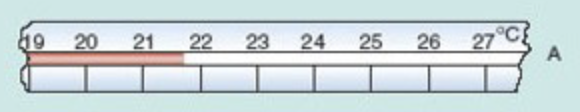
\includegraphics[width=0.4\textwidth]{Screenshot 2026-05-31 at 10.17.01 PM.png}
        \end{figure}
        The tool tells us that the temperature is 21\textdegree C, but we must estimate the last digit since our measurement is between the two graduations. The final measurement should be around 21.6\textdegree C, with some wiggle room for the inaccuracies of estimation. 
        \subsubsection{Significant Digits}
        Significant Digits are the digits that we know are accurate, and their rules help us make accurate calculations and round appropriately while maintaining as much precision as possible. A digit is significant if, it is not zero, a zero between significant digits,  or a zero after a decimal point and after other significant digits. For AP Chemistry, you are correct if you are within once significant digit of accuracy. 
        \subsubsection{Extensive vs. Intensive Properties}
        A property is Extensive if it depends on the amount of a sample. Things like mass, volume, weight. A property is Intensive if it is independent on the amount of material present. Things like density or color. 
    \subsection{Particles and Reaction}
    Particles are tiny discrete pieces of matter, things like atoms, protons, neutrons, and electrons are all particles. We can measure the amount of these particles through their mass.

    \subsubsection{Atoms}
    Atoms are the particles that are core to chemistry. Atoms are the building blocks that make up everything, but are themselves made up of smaller particles called protons, neutrons and electrons. Atoms are composed of a dense nucleus at the center of the atom that contains the protons and neutrons and an electron cloud that makes up majority of the volume and houses the electrons.

    Electrons, denoted \ce{e-} have a negative charge and a low mass. Their low mass makes them susceptible to greater acceleration and therefore the move very fast in the electron cloud. Inside this cloud they exist at certain stable energy levels

    Protons, denoted \ce{p+}, are positively charged particles that live in the nucleus. They have a mass of 1 amu, much larger than the tiny electron. The number of protons in a nucleus determines the element through the atomic number, which equals the number of protons.

    Neutrons, denoted \ce{n^0}, are neutrally charged particles that live in the nucleus, they also have a mass of 1 amu. They help hold the nucleus together, acting as a sort of glue. There can be different numbers of neutrons for the same number of protons and the different configurations are called isotopes.

    Ions are atoms with a non-neutral charge due to an imbalance of electrons and neutrons. The charge is written as a superscript to the left of the atomic symbol. 

    Isotopes are the different variations of atoms with the same atomic number but different weights. They are written as the symbol-mass\# where the mass number is written in amu or atomic mass units. The average atomic mass of an element is the weighted average of the masses of its isotopes, based on their natural abundance. One graph that shows this is the mass spectra graph, which shows the abundance of each isotope based on the mass number.

    Atomic symbols can hold all of this information by including the mass number in the top left,the atomic number in the bottom left, and the charge in the top right.
    \[\ce{_6^12C^0}\]
    The above example represents a neutral Carbon-12 atom with 6 protons, 6 electrons, and 6 neutrons. In general the atomic symbol for any atom is given by
    \[_{\text{p}^+}^{\text{p}^+ + \text{n}^0}\text{X}^{\text{p}^+ - \text{e}^-}\]
    where the symbol X would be replaced to match the symbol associated with the atomic number. 

    \subsubsection{Bonding}
    Atoms form bonds to obtain a lower energy by filling their outer layer of electrons. This is because a full outer electron shell provides a more stable configuration for the atom. Nobel gases already have a full outer layer and that is why they are so unreactive. Atoms go about bonding in to different ways, Covalent Bonds and Ionic Bonds.

    In an Ionic bond one atom gives up some of its electrons to another atom forming two ions, a positive cation and a negative anion. In an ionic compound electrons are exchanged until both atoms have a full shell and the resulting compound has a ratio of ions resulting from their charges. The name of ionic compounds come from the name of the cation followed by the name of the anion changed so that it ends with -ide (oxide, fluoride, ect). Some cations have multiple charges that can be found in nature, when that happens we differentiate between them by putting roman numerals in the name. For example Iron has both 3+ and 2+ charges in nature, so we write \ce{Fe_2O_3} as Iron(iii) oxide since the iron ion \ce{Fe^3+} has a charge of 3+. There are also certain polyatomic ions that are made up of several atoms bound with covenant bonds such as \ce{NH4+} or \ce{NO3-} which have their own names. Below is a table containing the common polyatomic ions.
    \begin{table*}[h]
        \centering
        \begin{tabular}{c c c}
            Name & Chemical Formula & Charge \\
            \hline
            Ammonium & \ce{NH4+} & 1+ \\
            Acetate & \ce{C2H3O2-} & 1- \\
            Carbonate & \ce{CO3^2-} & 2- \\
            Chlorate & \ce{ClO3-} & 1- \\
            Chlorite & \ce{ClO2-} & 1- \\
            Chromate & \ce{CrO4^2-} & 2- \\
            Cyanide & \ce{CN-} & 1- \\
            Dichromate & \ce{Cr2O7^2-} & 2- \\
            Hydrogen Carbonate (Bicarbonate) & \ce{HCO3-} & 1- \\
            Hydrogen Sulfate & \ce{HSO4-} & 1- \\
            Hydride & \ce{H-} & 1- \\
            Hypochlorite & \ce{ClO-} & 1- \\
            Nitrate & \ce{NO3-} & 1- \\
            Nitrite & \ce{NO2-} & 1- \\
            Perchlorate & \ce{ClO4-} & 1- \\
            Permanganate & \ce{MnO4-} & 1- \\
            Peroxide & \ce{O2^2-} & 2- \\
            Phosphate & \ce{PO4^3-} & 3- \\
            Sulfate & \ce{SO4^2-} & 2- \\
            Sulfite & \ce{SO3^2-} & 2- \\
            Thiosulfate & \ce{S2O3^2-} & 2- \\
        \end{tabular}
        \caption{Polyatomic Ions Names and Chemical Formula}
    \end{table*}

    The charge taken by an atom is given by its oxidation number which can vary but does have a trend based on an elements position on the periodic table. Metals have positive oxidation numbers, transition metals typically have more than one oxidation number, non-metals and semi-metals have both positive and negative oxidation numbers, no element exists in a compound with an oxidation number greater than +8 and the most negative oxidation numbers equals the group number - 8. Nobel gases have no oxidation number as they do not form ions naturally. Below in \ref{table:OxidationNumbers} is a list of the first few elements and their possible oxidation numbers.
    
    Covalent bonds are formed when two atoms share electrons. The shared electrons allow both atoms to fill their outer shell and achieve a lower energy state. Covalent bonds can be single bonds, where one pair of electrons is shared, double bonds where two pairs of electrons are shared, and triple bonds where three pairs of electrons are shared. 
    \subsubsection{Advanced Compound Naming}
    The oxidation numbers of atoms also relate to the naming of polyatomic ions. The prefixes and suffixes for the polyatomic ion are based on the number of oxygen atoms and by extension the oxidation number of the central atom. The suffix -ate is used for the most common ion, -ite is used for the ion with one less oxygen, and hypo- and per- are used for ions with two less or two more oxygen atoms respectively. For example, the nitrate ion \ce{NO3-} has an oxidation number of +5 for nitrogen, so the nitrite ion \ce{NO2-} has an oxidation number of +3. The perchlorate ion \ce{ClO4-} has an oxidation number of +7, so the chlorate ion \ce{ClO3-} has an oxidation number of +5, the chlorite ion \ce{ClO2-} has an oxidation number of +3, and the hypochlorite ion \ce{ClO-} has an oxidation number of +1. The atoms that have polyatomic ions ending in the suffix -ate and 4 oxygen atoms form two squares called slivka squares, centered around niobium and arsenic and containing the 8 surrounding elements. All other atoms form -ate compounds with 3 oxygen atoms. The exception to this is Manganese which forms a -ate compound with 4 oxygen atoms, \ce{MnO4-}. 
    
    As hydrogen are added to these polyatomic ions, the name gains the prifix hydrogen or dihydrogen and the charge increases by 1 for each hydrogen added. For example, the carbonate ion \ce{CO3^2-} becomes the hydrogen carbonate ion \ce{HCO3-} with one hydrogen and the dihydrogen carbonate ion \ce{H2CO3} with two hydrogens. The sulfate ion \ce{SO4^2-} becomes the hydrogen sulfate ion \ce{HSO4-} with one hydrogen and the dihydrogen sulfate ion \ce{H2SO4} with two hydrogens. Another prefix that is commonly used is bi- which is used for ions with one hydrogen, such as the bicarbonate ion \ce{HCO3-} and the bisulfate ion \ce{HSO4-}.

    When naming an acid, the name of the acid depends on the name of the anion. If the anion ends in -ide, the acid name begins with hydro- and ends with -ic. For example, \ce{HCl} is hydrochloric acid because the anion is chloride. If the anion ends in -ite, the acid name ends with -ous. For example, \ce{HNO2} is nitrous acid because the anion is nitrite. If the anion ends in -ate, the acid name ends with -ic. For example, \ce{HNO3} is nitric acid because the anion is nitrate.

    Some ionic compounds also form complexes with water adding a third word to the name. Hydrates are ionic compounds that have a specific number of water molecules attached to them. The number of water molecules is indicated by a prefix and the word hydrate. For example, \ce{CuSO4*5H2O} is copper(II) sulfate pentahydrate because it has 5 water molecules attached to each formula unit of copper(II) sulfate.

    To name a covalent compound, we use the prefixes mono-, di-, tri-, tetra-, penta-, hexa-, hepta-, octa-, nona-, and deca- to indicate the number of atoms of each element in the compound. The first element is named using its full name, while the second element is named using its root and the suffix -ide. For example, \ce{CO2} is carbon dioxide because it has one carbon atom and two oxygen atoms. \ce{N2O4} is dinitrogen tetroxide because it has two nitrogen atoms and four oxygen atoms. The prefix mono- is typically omitted for the first element, so \ce{CO} is carbon monoxide, not monocarbon monoxide.

    In AP chemistry it is also expected that you know the names of the simple organic alkanes, which are hydrocarbons with only single bonds. The names of the alkanes are based on the number of carbon atoms in the molecule, with the suffix -ane. For example, \ce{CH4} is methane because it has one carbon atom, \ce{C2H6} is ethane because it has two carbon atoms, \ce{C3H8} is propane because it has three carbon atoms, and \ce{C4H10} is butane because it has four carbon atoms. The names of alkanes with more than four carbon atoms are based on Greek prefixes for the number of carbon atoms, such as pentane for five carbon atoms, hexane for six carbon atoms, and so on.

    \subsubsection{Periodic Trends}
    The periodic table is organized in a way that allows us to predict the properties of elements based on their position. The periodic trends are patterns in the properties of elements that occur as you move across a period or down a group in the periodic table. Some of the most important periodic trends include atomic radius, ionization energy, electronegativity, and electron affinity.

    Atomic radius is the size of the atom. The atomic radius increases down towards the left, with the largest atom being Francium. 

    Electronegativity is the ability of an atom to attract electrons in a chemical bond. Electronegativity increases up towards the right, with the most electronegative element being Fluorine.

    Ionization energy is the energy required to remove an electron from an atom. Ionization energy increases up towards the right, with the highest ionization energy being Helium.

    Electron affinity is the energy change that occurs when an atom gains an electron. Electron affinity increases up towards the right, with the highest electron affinity being Chlorine.

    In addition, we split the elements into metals, nonmetals, and metalloids. Metals are typically found on the left side of the periodic table and are characterized by their ability to conduct electricity, malleability, and ductility. Nonmetals are typically found on the right side of the periodic table and are characterized by their lack of conductivity, brittleness, and high ionization energies. Metalloids are elements that have properties of both metals and nonmetals and are typically found along the zig-zag line that separates metals and nonmetals on the periodic table.
    \subsection{Stoichiometry and the Mole}
        \subsubsection{Dimensional Analysis}
        Dimensional analysis is a method of converting between different units of measurement by using conversion factors. A conversion factor is a ratio of equivalent measurements that can be used to convert from one unit to another. To use dimensional analysis, you begin by writing the known value that you wish to convert, then multiply by a ratio with the unit you are canceling on opposite sides. For example to convert 5 kg to grams, you would write
\begin{equation*}
    5 \text{ kg} \times \frac{1000 \text{ g}}{1 \text{ kg}} = 5000 \text{ g}
\end{equation*}
        \subsubsection{Moles and Avogadro's Number}
        A mole is a unit of measurement that is used to count particles in chemistry. One mole is equal to 6.022 $\times$ 10$^{23}$ particles, which is called Avogadro's number. The mole is used to count atoms, molecules, ions, and other particles in chemistry. The molar mass of a substance is the mass of one mole of that substance, and it is typically expressed in grams per mole (g/mol). 
        \subsubsection{Standered Conditions}
        Many values in chemistry are measured at standered conditions, which are defined as a temperature of 0\textdegree C (273.15 K) and a pressure of 1 atm. At these conditions, one mole of an ideal gas occupies a volume of 22.4 liters. This is known as the molar volume of an ideal gas at standard temperature and pressure (STP).
        \subsubsection{Molarity, Density, Percent Composition}
        Concentration is a measure of the amount of solute dissolved in a given amount of solvent or solution. The most common unit of concentration is molarity (M), which is defined as the number of moles of solute per liter of solution. To find the molarity of a solution, you can use the formula:
        \begin{equation}\label{eq:molarity}
            M = \frac{n}{V}
        \end{equation}
        where $n$ is the number of moles of solute and $V$ is the volume of the solution in liters. This value is sometimes show in brackets. For example a 0.5 M solution of sodium chloride would be written as [NaCl] = 0.5 M.

        Density is a measure of how much mass is contained in a given volume. Density is not a measure of concentration because it uses the mass and volume of the entire solution, not just the solute. 

        The mole fraction can be used to convert between different concentrations. The mole fraction of a component in a solution is the ratio of the number of moles of that component to the total number of moles of all components in the solution. The mole fraction can be used to convert between molarity and mass percent, or between molarity and density.

        Parts per million (ppm) is a unit of concentration that is used to express very dilute concentrations. One ppm is equal to one part of solute per million parts of solution, which is equivalent to 1 mg of solute per liter of solution for aqueous solutions.

        Percent Composition is a way to express the concentration of a component in a solution as a percentage. It is calculated by dividing the mass of the component by the total mass of the solution and multiplying by 100\%.
        \subsubsection{Empirical and Molecular Formulas}
        The empirical formula for a compound is the ratio of atoms in a molecule. To find the empirical formula from percent composition or mass, divide each percent or mass by the corresponding atomic mass, then divide all by the smallest value to get the simplest whole number ratio. Rounding may be necessary to get whole numbers, and if the ratio is close to a common fraction such as 1.5, you can multiply all ratios by the denominator of that fraction to get whole numbers.
        To find the molecular formula from the empirical formula, you need to know the molar mass of the compound. Divide the molar mass by the empirical formula mass to get a whole number, then multiply the subscripts in the empirical formula by that whole number to get the molecular formula.
        \subsubsection{Hydrated Formulas}
        When trying to find the formula of a hydrate from mass or percent composition, you can use the same steps for finding the empirical formula, instead using the molar mass of water (18.015 g/mol) for the water component. The resulting formula will be in the form of \ce{X*YH2O} where X is the formula of the anhydrous compound and Y is the number of water molecules per formula unit of the anhydrous compound.
        \subsubsection{Dilutions}
        When diluting a solution, the number of moles remains constant while the concentration changes. The relationship between the initial and final concentrations and volumes can be expressed with the formula:
        \begin{equation}\label{eq:dilution}
            M_1V_1 = M_2V_2
        \end{equation}
        where $M_1$ and $V_1$ are the initial molarity and volume, and $M_2$ and $V_2$ are the final molarity and volume after dilution.
\section{Reactions}
A chemical reaction is the process of bonds breaking and forming to rearrange atoms in molecules. There are the same number of atoms on both sides of a chemical reaction because of the conservation of mass. In AP chemistry there are a few new topics in reactions that are new including redox reactions and their corresponding half reactions, net ionic reactions, and the reaction categories. 

Reactants are the starting materials in a chemical reaction, while products are the substances that are formed as a result of the reaction. Some reactions also contain a catalyst, which is a substance that speeds up the reaction without being consumed in the process. This is accomplished by lowering the activation energy of the reaction.

There are many different arrows used to symbolize reactions, including a standard arrow $\rightarrow$ which indicates a reaction that goes to completion, a double arrow $\rightleftharpoons$ which indicates a reaction goes to equilibrium, and a reversible arrow $\leftrightarrows$ which indicates a reaction that can go in either direction. In addition multiple arrows are used to indicate several steps occur $\substack{\quad\quad\rightarrow\\[-1em]\quad \rightarrow \\[-1em] \rightarrow}$ and a single arrow with a line through it $\nrightarrow$ is used to indicate a reaction that does not occur. It is important to not confuse the double arrow, the equilibrium arrow or the resonance arrow $\leftrightarrow$ which indicates a molecule that can be represented by multiple Lewis structures.

\subsection{Physical vs Chemical Changes}
A physical change has no effect on the atoms or molecules of a substance. Instead a physical change only changes the physical properties of a substance, such as its state of matter, shape, or size. Examples of physical changes include melting, boiling, freezing, cutting, and dissolving. A chemical change on the other hand is a change that results in the formation of new substances with different properties. Chemical changes involve the breaking and forming of chemical bonds between atoms. Examples of chemical changes include combustion, rusting, and digestion. Both involve energy exchanges, but chemical changes typically involve larger energy changes than physical changes. Physical changes are easily reversible, while chemical changes are often irreversible\footnote{It is possible to reverse a chemical change, but the energy required to do so is often nearly unachievable in reality.}
\subsection{Reaction Types}
\subsubsection{Clasical Reaction Types}
The classic reaction types are synthesis, decomposition, combustion, single replacement, and double replacement. In a synthesis reaction, two or more reactants combine to form a single product.
\[\ce{A + B -> AB}\]
In a decomposition reaction, a single reactant breaks down into two or more products.
\[\ce{AB -> A + B}\]
In a combustion reaction, a substance reacts with oxygen to produce energy in the form of heat and light.
\[\ce{C_xH_y + O2 -> CO2 + H2O}\]
A single replacement reaction is a reaction where one element replaces another element in a compound.
\[\ce{A + BC -> AC + B}\]
A double replacement reaction is a reaction where the positive and negative ions of two compounds switch places tor form two new compounds.
\[\ce{AB + CD -> AD + CB}\]
\subsubsection{Modern Reaction Types}
The modern reaction types that are more commonly used in AP chemistry are combustion, acid-base, redox, and precipitation reactions. The combustion reaction is the same as the classic combustion reaction. 

Combustion reactions are exothermic and are organic redox reactions. They always have some hydrocarbon and oxygen as reactants and carbon dioxide and water as products.

Acid-base, redox, and precipitation reactions all occur in solution. Since they occur in solution and have many ions that don't interact in the reaction, we use net ionic equations to represent the reaction. In a net ionic equation, we separate all ions that disassociate, writing out the ions as individual reactants or products. For example $\ce{HCl_{(aq)}}$ becomes $\ce{H+_{(aq)} + Cl-_{(aq)}}$. Then we cancel out any spectator ions that appear on both sides of the equation, leaving only the ions that are directly involved in the reaction. If a compound is not dissolved, it is not disassociated and therefore kept together as a single reactant or product.  
\subsubsection{Redox Reactions}\label{sec:OxidationReduction}
The classical single replacement, synthesis, and decomposition reactions become redox reactions.Redox reactions involve the transfer of electrons between reactants. If an element is oxidized, it loses electrons and if it is reduced, it gains electrons. This may seem counter intuitive but this is because the term reduce refers to the oxidation number, which gets lower with more electrons. A mnemonic used to memorize this is OIL RIG, which stands for Oxidation Is Loss, Reduction Is Gain. In a redox reaction, one reactant is oxidized and another reactant is reduced. The oxidation and reduction half reactions can be written separately to show the transfer of electrons more clearly.
In a half reaction the reactants and products are separated into two reactions, one for oxidation and one for reduction. We then ballance both sides of the half reaction by adding electrons to both sides to balance the charge, and then we can combine the two half reactions to get the overall redox reaction. For the reaction between Iron(ii) and Copper(iv) ions, the half reactions would be
\begin{align*}\ce{Fe^2+ -> Fe^3+ + e-} \\
\ce{Cu^4+ + 3e- -> Cu+}\end{align*}
Then we can multiply the first half reaction by 3 to get the same number of electrons in both reactions
\begin{align*}\ce{3Fe^2+ -> 3Fe^3+ + 3e-} \\
\ce{Cu^4+ + 3e- -> Cu+}\end{align*}
Then we can add the two half reactions together to get the overall redox reaction
\[\ce{3Fe^2+ + Cu^4+ -> 3Fe^3+ + Cu+}\]
It is usually easy to figure out what the products of a redox reaction will be using the common oxidation numbers, and from there figure out the half reactions. There are some which are more difficult however including Permanganate and Dichromate redox reactions. These half reactions along with others only occur in acidic or basic solutions, in which case you can balance them using $\ce{H+}$ or $\ce{OH-}$ ions respectively. For example, the half reaction for the reduction of permanganate in acidic solution is
\[\ce{MnO4- + 8H+ + 5e- -> Mn^2+ + 4H2O}\]
A table containing the common redox half reactions can be found below in \ref{table:StandardPotential}
\subsubsection{Precipitation and Acid-Base Reactions}
Double replacement reactions become either acid-base reactions or precipitation reactions. Acid base reactions involve the reaction of an acid and a base to produce water and a salt. 
Precipitation reactions involve the reaction of two aqueous solutions to produce an insoluble solid called a precipitate. The precipitate is a insoluble compound that forms when two aqueous solutions are mixed together. 
\subsection{Solubility Rules}
The factors that affect solubility include the amount of solvent and solute along with pressure, the substances, and the temperature. The most common solvent is water and is a requirement for many chemical reactions. There are a few general rules for weather an ionic compound is soluble in water. These rules are as follows.
\begin{enumerate}
    \item An ionic compound is always soluble if it contains
    \begin{itemize}
        \item A nitrate ion (\ce{NO3-})
        \item An acetate ion (\ce{C2H3O2-})
        \item An alkali metal cation (\ce{Li+}, \ce{Na+}, \ce{K+}, \ce{Rb+}, \ce{Cs+})
        \item An ammonium ion (\ce{NH4+})
        \item A chlorate ion (\ce{ClO3-}, \ce{ClO4-})
    \end{itemize}
    \item An ionic compound is usually soluble if it contains
    \begin{itemize}
        \item A halide ion (\ce{Cl-}, \ce{Br-}, \ce{I-}) except when paired with \ce{Ag+}, \ce{Hg^2+}, \ce{Pb2^2+}, or \ce{Cd^2+}
        \item A sulfate ion (\ce{SO4^2-}) except when paired with \ce{Ca^2+}, \ce{Sr^2+}, \ce{Ba^2+}, \ce{Ra^2+}, \ce{Pb2^2+}, or \ce{Ag+}
    \end{itemize}
    \item An ionic compound is usually insoluble if it contains
    \begin{itemize}
        \item A carbonate ion (\ce{CO3^2-})
        \item A phosphate ion (\ce{PO4^3-})
        \item A oxide or sulfide ion (\ce{O^2-}\ce{S^2-})
        \item A hydroxide ion (\ce{OH-})
    \end{itemize}
    Except when paired with an alkali metal or ammonium ion, in which case they are soluble.
\end{enumerate}

An ionic compound dissociates if it is soluble or if it is a strong acid or base, otherwise it will not dissociate. These compounds that disassociate are called strong electrolytes, while those that do not are called weak electrolytes. This is because disassociated ions allow water to conduct electricity. 
\subsubsection{Strong vs Weak Acids and Bases}
A strong acid is an acid that completely disassociates in water, while a weak acid is an acid that only partially disassociates in water. Similarly, a strong base is a base that completely disassociates in water, while a weak base is a base that only partially disassociates in water. The strength of an acid or base is determined by its ability to donate or accept protons.
The strong acids and bases are as listed below. 
\begin{table}[h]
\label{StrongAcidsBases}
\centering
\begin{tabular}{c c}
\textbf{Strong Acids} & \textbf{Strong Bases} \\
\hline
\ce{HCl} & \ce{LiOH} \\
\ce{HBr} & \ce{NaOH} \\
\ce{HI} & \ce{KOH} \\
\ce{HNO3} & \ce{RbOH} \\
\ce{HClO4} & \ce{CsOH} \\
\ce{HClO3} & \ce{Ca(OH)2} \\
\ce{H2SO4} & \ce{Sr(OH)2} \\
 & \ce{Ba(OH)2} \\
\end{tabular}
\caption{Strong Acids and Bases}
\end{table}
Some common examples of weak acids and bases include acetic acid (\ce{CH3COOH}), hydrofluoric acid (\ce{HF}), carbonic acid (\ce{H2CO3}), Aluminum hydroxide (\ce{Al(OH)3}), and Iron(iii) hydroxide (\ce{Fe(OH)3}). The number of hydrogens that can be donated by an acid or accepted by a base is the proticity of the acid or base. A monoprotic acid can donate one hydrogen, a diprotic acid can donate two hydrogens, and a triprotic acid can donate three hydrogens. The same applies to bases with accepting hydrogens.
\subsubsection{The Forces Behind Solubility}
The solubility rules come from the interactions between the ions and water molecules and is governed by coulomb's law. 
\begin{equation}
    F = k \frac{q_1 q_2}{r^2}\label{eq:coulombs}
\end{equation}
While AP chemistry does not require you to use coulomb's law in calculations you need to understand how it relates to many key ideas including solubility and periodic trends. Coulomb's law states that the force of attraction or repulsion between two charged particles is directly proportional to the product of their charges and inversely proportional to the square of the distance between them. This means that ions with higher charges will have stronger interactions with water molecules, making them more soluble. 
\subsection{Titrations}
A titration is a laboratory technique used to determine the concentration of an unknown solution by reacting it with a solution of known concentration. In AP chemistry there are two main types of titrations, acid-base titrations and redox titrations. Both use an indicator to determine the end point of the titration, and stoichiometry to determine the concentration of the unknown solution. To calculate the concentration of the unknown solution, write out the chemical reaction that is occurring, and use stoichiometry to convert the volume of solution added to find the moles of solute in the unknown solution, then divide by the volume of the unknown solution to find the molarity.
\section{Kinetics}
Kinetics is the study of the rate or speed of reactions. The main factors that affect the rate of a reaction are, the concentrations of the reactants, the surface area of an solid reactants, the phase of the reactants, the temperature, and the presence of a catalyst. 
\subsection{Collision Theory}
Collision theory states that for a reaction to occur, the reactant particles must collide with each other with sufficient energy and the correct orientation. The minimum energy required for a reaction to occur is called the activation energy. The more collisions that occur, the more likely it is that they will be successful and lead to a reaction. Therefore since increasing the concentration of reactants increases the number of collisions, it will increase the rate of the reaction\footnote{If it is hard to see why an increased concentrations will cause more collisions, think of the ideal gas law. $PV=nRT$ if we divide both sides by $V$ we get $P=nRT/V$, and $n/V$ is the concentration. So $P=MRT$ and $P\propto M$}.
Similarly a larger surface area of a solid reactant allows for more collisions to occur, and therefore increases the rate of the reaction. The phase of the reactants also affects the rate of the reaction, as reactions between gases tend to be faster than reactions between solids or liquids due to the increased mobility of gas particles.
\subsubsection{Maxwell Boltzmann Curves}
Temperature is a measure of the average kinetic energy of the particles in a substance. Since it is an average some particles will have more energy and some will have less. The Maxwell Boltzmann curve shows the distribution of kinetic energies of particles in a substance at a given temperature. 
\begin{figure}[h]
    \centering
    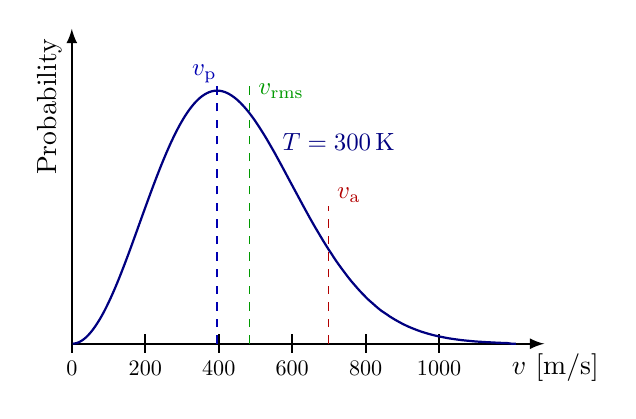
\begin{tikzpicture}
        \def\xmax{6.0}
        \def\ymax{4.0}
        \def\k{4500} % k = m/2k
        \def\xscale{0.14}
        \def\vn{2.6}
        \def\vmax{sqrt(300/\k)/\xscale}
        \def\vrms{sqrt(300/(2*\k/3))/\xscale}
        \coordinate (O) at (0,0);
        \coordinate (X) at (\xmax,0);
        \coordinate (Y) at (0,\ymax);
        
        % AXIS
        \draw[<->,thick]
            (Y) node[above left,rotate=90] {Probability} -- (0,0) -- (X) node[right=4,below] {$v$ [\si{m/s}]};
        \foreach %\x [evaluate={\c=sqrt(\k/0.00096); \v=(round(\x*\c/\xscale))}] in {1,...,3}{
                \i [evaluate={\v=int(\i*200);}] in {0,...,5}{
            \pgfmathsetmacro\x{\v*sqrt(0.00192)/\xscale/sqrt(\k))} % higher precision
            \tick{\x,0}{90} node[below,scale=0.8] {\v};
        }
        
        % LABELS
        \node[blue!50!black,above right=-1,scale=0.9] at (\vn,{\maxwell{\vn}{300}}) {$T=\SI{300}{K}$}; %f(x)
        \draw[myblue,dashed,thin]
            ({\vmax},0) coordinate (VM) --++ (0,{1.04*\maxwell{\vmax}{300}})
            node[myblue,left=1,above left=-4,scale=0.9] {$v_\text{p}$};
        \draw[mygreen,dashed,thin]
            ({\vrms},0) coordinate (VR) --++ (0,{1.04*\maxwell{\vmax}{300}})
            node[mygreen,above=2,below right=0,scale=0.9] {$v_\text{rms}$};
        \draw[myred,dashed,thin]
            ({\vrms+1},0) coordinate (VE) --++ (0,{0.6*\maxwell{\vrms}{300}})
            node[myred,below=2,above right=0,scale=0.9] {$v_\text{a}$};
        %\tick{VM}{90}; %node[myblue,right=1,below left=0,scale=0.85] {$v_\text{p}$};
        %\tick{VE}{90}; %node[myred,left=1,below=-2,scale=0.85] {$\expval{v}$};
        %\tick{VR}{90}; %node[mygreen,below right=0,scale=0.85] {$v_\text{rms}$};
        
        % PLOT
        \draw[blue!50!black,thick,samples=100,smooth,variable=\x,domain=0.01:0.94*\xmax]
            plot(\x,{\maxwell{\x}{300}});
        
    \end{tikzpicture}
    \caption{Maxwell Boltzmann Curve}
    \label{fig:MaxwellBoltzmann}
\end{figure}
The highest point on the curve is the most common speed or kinetic energy, denoted in figure \ref{fig:MaxwellBoltzmann} as $v_\text{p}$. The speed with the average kinetic energy is the root mean square speed, denoted as $v_\text{rms}$. The formula to calculate the root mean squared speed is as follows;
\begin{equation}\label{eq:vrms}
v_\text{rms} = \sqrt{\frac{3RT}{M}}
\end{equation}
Where $R$ is the gas constant and $M$ is the molar mass of the gas. The minimum speed required for a reaction to occur is the activation energy, denoted as $v_\text{a}$. As the temperature increases, the curve flattens and shifts to the right, indicating that more particles have higher kinetic energies and therefore more particles have enough energy to overcome the activation energy barrier, leading to an increased rate of reaction. 
\begin{figure}[h]
    \centering
    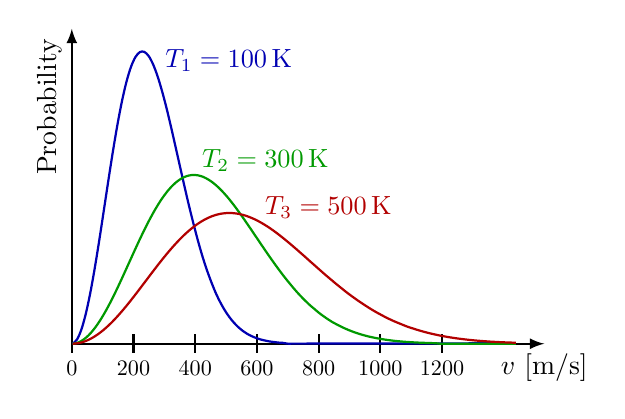
\begin{tikzpicture}
        \def\xmax{6.0}
        \def\ymax{4.0}
        \def\k{2000}
        \def\xscale{0.25}
        \def\vb{1.1}
        \def\vg{1.6}
        \def\vr{2.4}
        \coordinate (O) at (0,0);
        \coordinate (X) at (\xmax,0);
        \coordinate (Y) at (0,\ymax);
        
        % AXIS
        \draw[<->,thick]
            (Y) node[above left,rotate=90] {Probability} -- (0,0) -- (X) node[below] {$v$ [\si{m/s}]};
        \foreach \i [evaluate={\v=int(\i*200);}] in {0,...,6}{
            \pgfmathsetmacro\x{\v*sqrt(0.00192)/\xscale/sqrt(\k))} % higher precision
            \tick{\x,0}{90} node[below,scale=0.8] {\v};
        }
        
        % LABELS
        \node[bline,above right=-1,scale=0.95] at (\vb,{\maxwell{\vb}{100}}) {$T_1=\SI{100}{K}$};
        \node[gline,above right=-2,scale=0.95] at (\vg,{\maxwell{\vg}{300}}) {$T_2=\SI{300}{K}$};
        \node[rline,above right=-2,scale=0.95] at (\vr,{\maxwell{\vr}{500}}) {$T_3=\SI{500}{K}$};
        
        % PLOT
        \draw[bline,samples=100,smooth,variable=\x,domain=0.01:0.94*\xmax]
            plot(\x,{\maxwell{\x}{100}});
        \draw[gline,samples=100,smooth,variable=\x,domain=0.01:0.94*\xmax]
            plot(\x,{\maxwell{\x}{300}});
        \draw[rline,samples=100,smooth,variable=\x,domain=0.01:0.94*\xmax]
            plot(\x,{\maxwell{\x}{500}});
  
    \end{tikzpicture}
    \caption{Maxwell Boltzmann Curves at different temperatures}
    \label{fig:MaxwellBoltzmann2}
\end{figure}
This can be seen in figure \ref{fig:MaxwellBoltzmann2}. It is also not uncommon to see maxwell boltzmann curves where speed is replaced by kinetic energy, but the same principles apply. Remember that kinetic energy is related to speed by
\begin{equation}\label{eq:KE}
    KE = \frac{1}{2}mv^2
\end{equation}
The effect of a catalyst on the Maxwell Boltzmann curve is to lower the activation energy, which allows more particles to have enough energy to react, increasing the rate of the reaction.
\subsubsection{Mechanisms}
Most reactions don't take one step, but instead a series of simple steps involving one collision. These simple steps are called elementary steps, and the series of steps is called the reaction mechanism. In the process of the reaction high energy radicals can be formed during transition states where the bonds are breaking and forming. These radicals are called intermediates and are used up in the following steps. Different steps in the mechanism can occur at different rates. The overall reaction is determined by the slowest of the steps, which is called the rate determining step. 
\subsection{Reaction Energy Diagrams}
A reaction energy diagram is a graph that shows the energy changes that occur during a chemical reaction. The x-axis represents the progress of the reaction, while the y-axis represents the energy of the system. 
\begin{figure}[h]
    \centering
    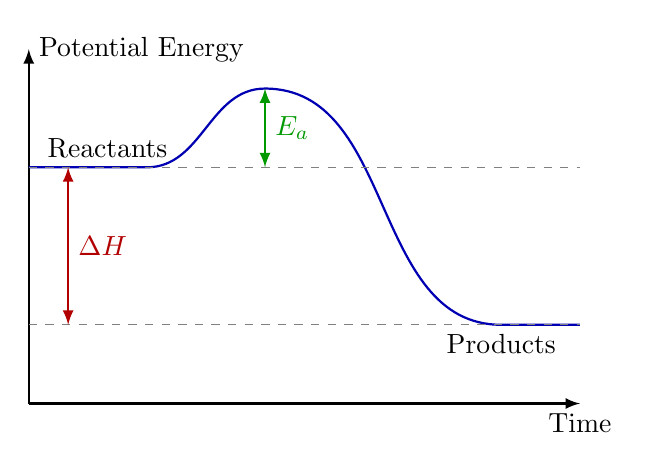
\begin{tikzpicture}
        \draw[->, thick] (0,0) -- (7,0) node[below] {Time};
        \draw[->, thick] (0,0) -- (0,4.5) node[above, right] {Potential Energy};
        
        % Energy curve for endothermic reaction
        \draw[thick, myblue] (0,3) -- (1.5,3) to[out=0,in=180] (3,4) to[out=0,in=180] (6,1) -- (7,1);

        \draw[dashed, gray] (0,3) -- (7,3);
        \draw[dashed, gray] (0,1) -- (7,1);

        \draw[<->, myred, thick] (0.5,3) -- (0.5,1) node[midway, right] {$\Delta H$};
        \draw[<->, mygreen, thick] (3,3) -- (3,4) node[midway, right] {$E_a$};

        \node[above] at (1,3) {Reactants};
        \node[below] at (6,1) {Products};
    \end{tikzpicture}
    \caption{Reaction Energy Diagram}
    \label{fig:ReactionEnergyDiagram}
\end{figure}
The value $\Delta H$ represents the change in enthalpy of the reaction (see section \ref{sec:enthalpy}), or the change in energy from the reactants to the products. $E_a$ represents the activation energy, or the energy barrier that must be overcome for the reaction to occur. When there are multiple steps in a reaction, there will be multiple peaks in the energy diagram.
\begin{figure}[h]
    \centering
    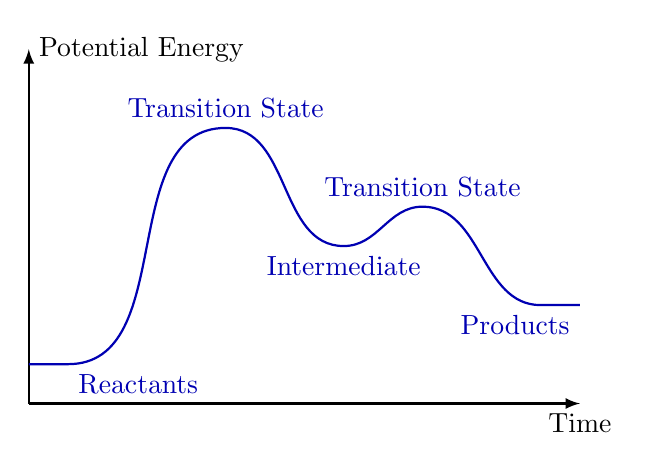
\begin{tikzpicture}
        \draw[->, thick] (0,0) -- (7,0) node[below] {Time};
        \draw[->, thick] (0,0) -- (0,4.5) node[above, right] {Potential Energy};
        
        % Energy curve for multi-step reaction
        \draw[thick, myblue] (0,0.5) -- (0.5,0.5) node[below right] {Reactants} to[out=0,in=180] (2.5,3.5) node[above] {Transition State} to[out=0,in=180] (4,2) node[below] {Intermediate} to[out=0,in=180] (5,2.5) node[above] {Transition State} to[out=0,in=180] (6.5,1.25) -- (7,1.25) node[below left] {Products};
    \end{tikzpicture}
    \caption{Multi-step Reaction Energy Diagram}
    \label{fig:MultiStepReactionEnergyDiagram}
\end{figure}
The highest peak corresponds to the step with the highest activation energy, which is the rate determining step. In figure \ref{fig:MultiStepReactionEnergyDiagram} the first step is the rate determining step since it has the highest activation energy.
\subsection{The Rate Law}
\subsubsection{Differential Rate Laws}
A rate law is an equation that relates the rate of a reaction to the concentrations of the reactants. The general form of a rate law for the elementary reaction \ce{mA + nB -> pC + qD} is as follows;
\begin{equation}\label{eq:rateLaw}
    \text{Rate} = k[A]^m[B]^n
\end{equation}
It is important to note that the exponents in the rate law are not necessarily the same as the coefficients in the balanced chemical equation, but instead come from the coefficients of the rate determining step in the mechanism. The value $k$ is a constant called the rate constant, which is specific to a particular reaction at a given temperature. 

For those who are familiar with calculus, the rate of a reaction can also be expressed as the derivative of the concentration of a reactant or product with respect to time. For example, for the reaction \ce{A -> B} the rate can be expressed as
\begin{equation}\label{eq:differentialRateLaw}
    \text{Rate} = -\frac{d[A]}{dt} = \frac{d[B]}{dt} = k[A]^m
\end{equation}
This is why these are called the differential rate laws, because they take the form of a derivative.

\subsubsection{Molecularity and Reaction Order}
The molecularity of an elementary reaction is the number of reactant particles that are involved in the reaction. A unimolecular reaction involves one reactant particle, a bimolecular reaction involves two reactant particles, and a termolecular reaction involves three reactant particles. It is very rare to have reactions with a molecularity greater than three. The order of a reaction is the sum of the exponents in the rate law for the overall reaction. A zero order reaction has a constant rate, a first order reaction has a rate that is directly proportional to the concentration of one reactant, and a second order reaction has a rate that is proportional to the square of the concentration of one reactant or the product of the concentrations of two reactants.

The order of a reactant can be found by comparing how the change to an initial concentration of a reactant affects the rate of the reaction. For example, if doubling the concentration of a reactant causes the rate to double, then the reaction is first order with respect to that reactant. If doubling the concentration causes the rate to quadruple, then the reaction is second order with respect to that reactant. If changing the concentration has no effect on the rate, then the reaction is zero order with respect to that reactant.

\subsubsection{Integrated Rate Laws}
The integrated rate law is an equation that relates the concentration of a reactant to time. The equation itself is based on the order of the reaction. For a zero order reaction, the integrated rate law is as follows;
\begin{equation}\label{eq:zeroOrder}
    [A] = -kt + [A]_0
\end{equation}
For a first order reaction, the integrated rate law is as follows;
\begin{equation}\label{eq:firstOrder}
    \ln{[A]} = -kt + \ln{[A]_0}
\end{equation}
For a second order reaction, the integrated rate law is as follows;
\begin{equation}\label{eq:secondOrder}
    \frac{1}{[A]} = kt + \frac{1}{[A]_0}
\end{equation}
Where $[A]_0$ is the initial concentration of the reactant. These equations can be used to determine the concentration of a reactant at any given time, or to determine the rate constant $k$ if the concentration at different times is known.

For those who are familiar with calculus, the integrated rate laws can be derived by using separation of variables to integrate the differential rate laws. 

We can also use the integrated rate laws to determine the order of a reaction by plotting the appropriate graph and seeing if it is linear. For example, if a plot of $[A]$ vs time is linear, then the reaction is zero order. If a plot of $\ln{[A]}$ vs time is linear, then the reaction is first order. If a plot of $1/[A]$ vs time is linear, then the reaction is second order.
\subsubsection{Half Life}
The half life of a reaction is the time it takes for the concentration of a reactant to decrease by half. The half life of a reaction can be determined from the integrated rate law. For a zero order reaction, the half life is given by
\begin{equation}\label{eq:halfLifeZero}
    t_{1/2} = \frac{[A]_0}{2k}
\end{equation}
For a first order reaction, the half life is given by
\begin{equation}\label{eq:halfLifeFirst}
    t_{1/2} = \frac{\ln{2}}{k}
\end{equation}
For a second order reaction, the half life is given by
\begin{equation}\label{eq:halfLifeSecond}
    t_{1/2} = \frac{1}{k[A]_0}
\end{equation}
\subsection{Arrhenius Equation}
The Arrhenius equation is a mathematical equation that describes the relationship between the rate constant of a reaction, the activation energy, and the temperature. The Arrhenius equation is not needed for the AP exam, but it is a useful equation to know for understanding how temperature affects the rate of a reaction. The Arrhenius equation is as follows;
\begin{equation}\label{eq:arrhenius1}
    k = Ae^{-\frac{E_a}{RT}}
\end{equation}
Where $A$ is the frequency factor, $E_a$ is the activation energy, $R$ is the gas constant, and $T$ is the temperature in Kelvin. The Arrhenius equation shows that as the temperature increases, the rate constant $k$ increases, which means that the rate of the reaction increases. 
Another common form of the Arrhenius equation is
\begin{equation}\label{eq:arrhenius2}
    \ln{k} = \ln{A} - \frac{E_a}{RT}
\end{equation}
This form of the equation is useful for plotting $\ln{k}$ vs $1/T$, which will yield a straight line with a slope of $-E_a/R$ and a y-intercept of $\ln{A}$.
To find the rate constant at a different temperature, we can use the following form of the Arrhenius equation;
\begin{equation}\label{eq:arrhenius3}
    \ln{\left(\frac{k_2}{k_1}\right)} = -\frac{E_a}{R}\left(\frac{1}{T_2} - \frac{1}{T_1}\right)
\end{equation}
Where $k_1$ and $k_2$ are the rate constants at temperatures $T_1$ and $T_2$ respectively.


\section{Equilibrium}
Equilibrium is deeply connected to kinetics and represents the state of a system where the forward and reverse reactions occur at the same rate, resulting in no net change in the concentrations of reactants and products. As the concentrations change over time, the system will eventually reach a point where the rates of the forward and reverse reactions are equal, and the concentrations of reactants and products remain constant. This state is known as chemical equilibrium.

The reason that equilibrium exists is because reactions are reversible, meaning that the products can react to form the reactants. Some reactions are more likely to proceed in one direction than the other, but eventually, the system will reach a point where the rates of the forward and reverse reactions are equal, and the concentrations of reactants and products remain constant. A common example of a reaction that is reversible is the disassociation of water:
\[\ce{2H2O_{(l)} <=> H3O+_{(aq)} + OH-_{(aq)}}\]

In order for a state to be in equilibrium, the system must be closed, meaning that no matter can enter or leave the system, or isolated, meaning that no matter or energy can enter or leave the system. The state of equilibrium is dynamic and is always a give and take trying to reach a balance. Both reactions are always occurring, but at equilibrium, they are occurring at the same rate, so there is no observable change. While catalysts do have an effect on the rate of a reaction, they do not have an effect on the equilibrium state of a reaction. Catalysts speed up both the forward and reverse reactions equally, so they do not change the position of equilibrium, but they do help the system reach equilibrium faster. There are certain catalysts that can help one direction of the reaction more than the other, but they are not common.

For any reaction there is always some amount of both reactants and products, even if it is a very small amount. The amount of each is dependent on the temperature and the exact reaction. A homogeneous equilibrium is an equilibrium where all the reactants and products are in the same phase. The process of reaching equilibrium has three phases, the initial phase when the reactants are first mixed, the kinetic region where the products are being formed and the reactants are being consumed, and the equilibrium region where the concentrations of reactants and products remain constant. It is important to remember that the concentrations of reactants and products at equilibrium are not necessarily equal, but they are constant. 

\subsection{Equilibrium Constant}
The equilibrium constant, $K_{eq}$, is a measure of the relative concentrations of reactants and products at equilibrium. It is defined by the following expression for a general reaction \ce{nA + mB <=> pC + qD}:
\begin{equation}\label{eq:Keq}
    K_{eq} = \frac{[C]^p[D]^q}{[A]^n[B]^m}
\end{equation}
This expression comes from the two rate laws for the forward and reverse reactions. The value $K_{eq}$ is a constant for a given reaction at a given temperature, and tells us about the position of equilibrium. If $K_{eq}$ is greater than 1, then the equilibrium favors the products, while if $K_{eq}$ is less than 1, then the equilibrium favors the reactants. Given any temperature, $K_{eq}$ is a constant, and will not change. 

The equilibrium constant for the reverse of any reaction can be expressed as the reciprocal of the equilibrium constant for the forward reaction. 

\subsection{Le Chatelier's Principle}
Le Chatelier's Principle states that if a system at equilibrium is subjected to a change in concentration, temperature, or pressure, the system will adjust itself to counteract the change and restore equilibrium. This principle can be used to predict how a system will respond to changes in conditions. Increasing concentration of a reactant or product will push the reaction to the other side. Decreasing concentration of a reactant or product will pull the reaction to the same side. To see how temperature affects equilibrium, we can treat temperature as a reactant or product. If the reaction is endothermic, then heat is a reactant, so increasing temperature will push the reaction to the products, while decreasing temperature will pull the reaction to the reactants. If the reaction is exothermic, then heat is a product, so increasing temperature will push the reaction to the reactants, while decreasing temperature will pull the reaction to the products. An increase in pressure will favor the side of the reaction with fewer moles of gas, while a decrease in pressure will favor the side of the reaction with more moles of gas. Similarly with volume, a decrease in volume will favor the side of the reaction with fewer moles of gas, while an increase in volume will favor the side of the reaction with more moles of gas. It is important to note that the changes do not come from a changing equilibrium constant, but rather from the system trying to restore equilibrium. The value of $K_{eq}$ does not change with changes in concentration, pressure, or volume.

\subsection{Other Equilibrium Constants}\label{sec:other_equilibrium_constants}
There are other equilibrium constants that are used to describe specific types of reactions. $K_{eq}$ or $K_c$ is used for general reactions using units of concentration. $K_p$ is used for reactions involving gases using units of pressure. $K_w$ is the equilibrium constant for the autoionization of water, which is equal to $1.0 \times 10^{-14}$ at 25°C. $K_{sp}$ is the solubility equilibrium constant, which is used to describe the solubility of compounds in water. $K_a$ is the acid dissociation constant, which is used to describe the strength of acids, while $K_b$ is the base dissociation constant, which is used to describe the strength of bases. The relationship between $K_a$ and $K_b$ for a conjugate acid-base pair is given by the equation $K_a \cdot K_b = K_w$.

If you wish to convert between $K_c$ and $K_p$, you can use the following equation:
\begin{equation}\label{eq:KcKp}
    K_p = K_c(RT)^{\Delta n}
\end{equation}
where $R$ is the ideal gas constant, $T$ is the temperature in Kelvin, and $\Delta n$ is the change in the number of moles of gas between the reactants and products.

\subsection{ICE Tables}
ICE tables are a useful tool for solving equilibrium problems. ICE stands for Initial, Change, and Equilibrium. The initial row represents the initial concentrations of the reactants and products before the reaction starts. The change row represents the changes in concentration that occur as the reaction proceeds towards equilibrium. The equilibrium row represents the concentrations of the reactants and products at equilibrium. By using the equilibrium constant expression and the information from the ICE table, we can solve for unknown concentrations or the value of the equilibrium constant.

Take for example the following reaction:
\[\ce{CO + H2O <=> CO2 + H2}\]
with an initial concentration of 1 M for all components and an equilibrium constant of 5.10. We can set up the following ICE table:
\begin{center}
    \begin{tabular}{l|c|c|c|c}
        & \ce{CO} & \ce{H2O} & \ce{CO2} & \ce{H2} \\
        \hline
        I & $1.00$ & $1.00$ & $1.00$ & $1.00$ \\
        C & & & & \\
        E & & & & \\
    \end{tabular}
\end{center}
Since $K_{eq} > 1$ we know that the reaction favors the products, so we can assume that the change in concentration of the reactants is $-x$ and the change in concentration of the products is $+x$. This gives us the following ICE table:
\begin{center}
    \begin{tabular}{l|c|c|c|c}
        & \ce{CO} & \ce{H2O} & \ce{CO2} & \ce{H2} \\
        \hline
        I & $1.00$ & $1.00$ & $1.00$ & $1.00$ \\
        C & $-x$ & $-x$ & $+x$ & $+x$ \\
        E & $1.00 - x$ & $1.00 - x$ & $1.00 + x$ & $1.00 + x$ \\
    \end{tabular}
\end{center}
We can then plug the equilibrium concentrations into the equilibrium constant expression to solve for $x$:
\begin{align*}
    K_{eq} &= \frac{[\ce{CO2}][\ce{H2}]}{[\ce{CO}][\ce{H2O}]} \\
    5.10 &= \frac{(1.00 + x)(1.00 + x)}{(1.00 - x)(1.00 - x)} \\
    5.10 &= \frac{(1.00 + x)^2}{(1.00 - x)^2} \\
    \sqrt{5.10} &= \frac{1.00 + x}{1.00 - x} \\
    1.00 + x &= \sqrt{5.10}(1.00 - x) \\
    1.00 + x &= \sqrt{5.10} - \sqrt{5.10}x \\
    x + \sqrt{5.10}x &= \sqrt{5.10} - 1.00 \\
    x(1 + \sqrt{5.10}) &= \sqrt{5.10} - 1.00 \\
    x &= \frac{\sqrt{5.10} - 1.00}{1 + \sqrt{5.10}} \\
    x &\approx 0.387 \text{ M}
\end{align*}
This means that at equilibrium, the concentration of CO and H2O will be approximately 0.613 M, while the concentration of CO2 and H2 will be approximately 1.387 M.

\subsubsection{x is Small Approximation}
In some cases, the value of $x$ may be very small compared to the initial concentrations, which can make the algebraic manipulation easier. In these cases, we can make the approximation that $1.00 - x \approx 1.00$ and $1.00 + x \approx 1.00$. This happens when $K_{eq}$ is very small and the initial concentrations are relatively large. If the change in concentration is less than 5\% of the initial concentration, then the approximation is valid. 
\subsection{The Reaction Quotient}
The reaction quotient, $Q$, is a measure of the relative concentrations of reactants and products at any point in time, not just at equilibrium. It is defined by the same expression as the equilibrium constant, but with the concentrations at any point in time:
\begin{equation}\label{eq:Q}
    Q = \frac{[C]^p[D]^q}{[A]^n[B]^m}
\end{equation}
By comparing the value of $Q$ to the value of $K_{eq}$, we can predict the direction in which the reaction will proceed to reach equilibrium. If $Q < K_{eq}$, then the reaction will proceed in the forward direction to produce more products. If $Q > K_{eq}$, then the reaction will proceed in the reverse direction to produce more reactants. If $Q = K_{eq}$, then the system is already at equilibrium and there will be no net change in concentrations.
\section{Aqueous}
Aqueous is the study of reactions in water. The properties of water allow for certain reactions to occur that would not occur otherwise. Acid base reactions are especially key to aqueous. 

\subsection{Definitions of Acids and Bases}
\subsubsection{Arrhenius}
The Arrhenius definition of acids and bases is the most basic. It states that an acid is a substance that increases the concentration of hydrogen ions in solution, while a base is a substance that increases the concentration of hydroxide ions in solution. The problems with this definition that made other definitions necessary are that it only applies to aqueous solutions and does not account for substances that can act as acids or bases in non-aqueous solvents. In addition, it does not account for substances that can act as both acids and bases (amphoteric substances).
\subsubsection{Brønsted-Lowry}
The Brønsted-Lowry definition of acids and bases is the most commonly used definition. It states that an acid is a substance that donates a proton (\ce{H+}) and a base is a substance that accepts a proton. This definition is more general than the Arrhenius definition and can be applied to non-aqueous solvents. It also accounts for amphoteric substances, which can act as both acids and bases.
\subsubsection{Lewis}\label{sec:lewis_acids_bases}
The Lewis definition of acids and bases is the most general definition. It states that an acid is a substance that accepts an electron pair and a base is a substance that donates an electron pair. While it is the most general definition, it is hard to grasp the concept of Lewis acids and bases.
\subsection{Conjugate Acids and Bases}
Acids and bases can be thought of as a pair of substances that are related to each other. When an acid donates a proton, it forms its conjugate base. When a base accepts a proton, it forms its conjugate acid. Take the following reaction as an example:
\[\ce{NH3_{(aq)} + H2O_{(l)} <=> NH4+_{(aq)} + OH-_{(aq)}}\]
In this reaction, \ce{NH3} is the base and \ce{H2O} is the acid. When \ce{NH3} accepts a proton from \ce{H2O}, it forms its conjugate acid, \ce{NH4+}. When \ce{H2O} donates a proton to \ce{NH3}, it forms its conjugate base, \ce{OH-}. These conjugate acids and bases themselves react with each other in a reversible reaction, which is why we use the double arrow in the reaction above. 

If an acid is strong, its conjugate base will be weak. If a base is strong, its conjugate acid will be weak. This is because a strong acid will completely dissociate in solution, leaving very little of the conjugate base to react with. Similarly, a strong base will completely dissociate in solution, leaving very little of the conjugate acid to react with. In reactions where the acid or base is strong, we can ignore the reverse reaction and use a single arrow instead of a double arrow. 
\subsection{pH and pOH}
pH is a measure of the acidity of a solution. It is defined as the negative logarithm of the hydrogen ion concentration:
\begin{equation}\label{eq:pH}
    \text{pH} = -\log[\ce{H+}]
\end{equation}
pOH is a measure of the basicity of a solution. It is defined as the negative logarithm of the hydroxide ion concentration:
\begin{equation}\label{eq:pOH}
    \text{pOH} = -\log[\ce{OH-}]
\end{equation}
The relationship between pH and pOH is given by the equation:
\begin{equation}\label{eq:pH_pOH}
    \text{pH} + \text{pOH} = 14
\end{equation}
This means that if you know the pH of a solution, you can calculate the pOH, and vice versa. It is important to remember that the relationship between pH and pOH is only valid for aqueous solutions at 25°C. 

Given these equations we can convert between pH and pOH, and also calculate the concentration of hydrogen ions or hydroxide ions in a solution if we know the pH or pOH.

\begin{align}
    [\ce{H+}] &= 10^{-\text{pH}} \label{eq:H+} \\
    [\ce{OH-}] &= 10^{-\text{pOH}} \label{eq:OH-}
\end{align}

And knowing the relationship between pH and pOH from equation \eqref{eq:pH_pOH}, we get the relationship between the concentration of hydrogen ions and hydroxide ions in solution:

\begin{equation}\label{eq:Kw}
    [\ce{H+}] [\ce{OH-}] = 10^{-14}
\end{equation}

\subsection{Equilibrium for Aqueous}

Water is a very special molecule. It can act as both an acid and a base, which is why it is called amphoteric. In fact water can even react with itself in a process called autoionization, where one water molecule donates a proton to another water molecule, forming a hydronium ion (\ce{H3O+}) and a hydroxide ion (\ce{OH-}):
\[\ce{2H2O_{(l)} <=> H3O+_{(aq)} + OH-_{(aq)}}\]
In aqueous solutions, we can write the equilibrium constant for the dissociation of water as:

\begin{equation}
    K_w = [\ce{H+}] [\ce{OH-}] = 10^{-14}
\end{equation}

This is the reason that the relationship between pH and pOH is given by equation \eqref{eq:pH_pOH}.
For strong acids and bases, we can ignore the reverse reaction and use a single arrow instead of a double arrow. In this case there is no need to consider the equilibrium constant, as the reaction will go to completion. However, for weak acids and bases, we need to consider the equilibrium constant. In section \ref{sec:other_equilibrium_constants} we mentioned the equilibrium constant for the dissociation of a weak acid, which is called the acid dissociation constant, $K_a$. Similarly, we can define the base dissociation constant, $K_b$, for the dissociation of a weak base. The value of $K_a$ is the equilibrium constant for a reaction of the form
\[\ce{HA_{(aq)} + H2O_{(l)} <=> A-_{(aq)} + H3O+_{(aq)}}\]
where \ce{HA} is a weak acid and \ce{A-} is its conjugate base. The value of $K_b$ is the equilibrium constant for a reaction of the form
\[\ce{B_{(aq)} + H2O_{(l)} <=> BH+_{(aq)} + OH-_{(aq)}}\]
where \ce{B} is a weak base and \ce{BH+} is its conjugate acid.
This gives us that the equilibrium constant for the dissociation of a weak acid is given by:

\begin{equation}\label{eq:Ka}
    K_a = \frac{[\ce{A-}] [\ce{H3O+}]}{[\ce{HA}]}
\end{equation}

And the equilibrium constant for the dissociation of a weak base is given by:

\begin{equation}\label{eq:Kb}
    K_b = \frac{[\ce{BH+}] [\ce{OH-}]}{[\ce{B}]}
\end{equation}

The relationship between $K_a$ and $K_b$ is given by the equation:

\begin{equation}\label{eq:KaKb}
    K_a K_b = K_w
\end{equation}

This means that if you know the value of $K_a$ for a weak acid, you can calculate the value of $K_b$ for its conjugate base, and vice versa. 

\subsection{Titrations}

Titrations are a common laboratory technique used to determine the concentration of an unknown acid or base. 

\subsubsection{Titration Curves}

A titration curve is a graph of the pH of a solution as a function of the volume of titrant added. The shape of the titration curve can provide information about the strength of the acid or base being titrated. Some points of interest on a titration curve include the equivalence point (sometimes called inflection point), which is the point at which the amount of titrant added is stoichiometrically equivalent to the amount of acid or base being titrated, the endpoint, which is the point at which the indicator changes color, and the starting point, which is the initial pH of the solution before any titrant is added.

\begin{figure}[h]
    \centering
    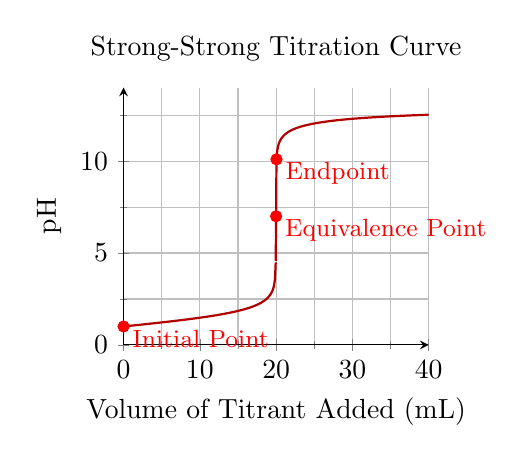
\begin{tikzpicture}[
        declare function={
            f(\x)= -log10(
                (sqrt(((\Mb*\x/(\Va+\x))+\ka)^2 + 4*\ka*((\Ma*\Va)-(\Mb*\x))/(\Va+\x)) - ((\Mb*\x/(\Va+\x))+\ka))/2
            );
            g(\x)=14+log10(
                (((\x*\Mb)-(\Va*\Ma))/(\Va+\x)) +
                (
                    sqrt(
                        ((((\x*\Mb)-(\Va*\Ma))/(\Va+\x)) + (10^(-14)/\ka))^2
                        + 4*(10^(-14)/\ka)*\Ma*\Va
                    )
                    - ((((\x*\Mb)-(\Va*\Ma))/(\Va+\x)) + (10^(-14)/\ka))
                )/2
            );
            h(\x)=14+log10(((sqrt(((10^(-14)/\ka)+10^(-7))^2 - 2 * \Ma * (10^(-14)/\ka))-((10^(-14)/\ka)+10^(-7)))/2)+10^(-7));
        }
    ]
        \pgfmathsetmacro{\ka}{13}
        \pgfmathsetmacro{\Ma}{0.1}
        \pgfmathsetmacro{\Mb}{0.1}
        \pgfmathsetmacro{\Va}{20}
        \pgfmathsetmacro{\kb}{(10^(-14)/\ka)}
        \begin{axis}[
            xlabel={Volume of Titrant Added (mL)},
            ylabel={pH},
            title={Strong-Strong Titration Curve},
            grid=both,
            axis lines=left,
            minor tick num=1,
            width=0.45\textwidth,
            height=0.4\textwidth,
            ymin=0,
            ymax=14,
        ]
        % Add the titration curve
        \addplot[
            domain=0:{(\Va*\Ma/\Mb)-0.05},
            samples=200,
            thick,
            color=myred,
        ]{f(x)};
        \addplot[
            domain={(\Va*\Ma/\Mb)+0.05}:{2*\Va},
            samples=200,
            thick,
            color=myred,
        ]{g(x)};
        \addplot[mark=none, color=myred, thick] coordinates 
        {
            ({(\Va*\Ma/\Mb)-0.05}, {f(x)})
            ({(\Va*\Ma/\Mb)},{h(x)})
            ({(\Va*\Ma/\Mb)+0.05}, {g(x)})
            };
        \addplot[
                mark=*,
                only marks, 
                color=red, 
                nodes near coords, 
                point meta=explicit symbolic,
                nodes near coords style={below right, node font=\small, inner ysep=1pt},
                ] coordinates 
        {
            ({(\Va*\Ma/\Mb)}, {h(x)}) [Equivalence Point]
            ({(\Va*\Ma/\Mb)+0.05}, {g(x)}) [Endpoint]
            ({0}, {f(0)}) [Initial Point]
        };
        \end{axis}
    \end{tikzpicture}
    \caption{A titration curve for a strong acid being titrated with a strong base.}
    \label{fig:titration_curve}
\end{figure}

Figure \ref{fig:titration_curve} shows a titration curve for a strong acid being titrated with a strong base. The initial point is at a low pH, and as the titrant is added, the pH increases until it reaches the equivalence point, where the pH is 7. After the equivalence point, the pH continues to increase as more titrant is added. The endpoint is slightly after the equivalence point, which is where the indicator changes color. If instead a strong base was being titrated with a strong acid, the initial point would be at a high pH, and as the titrant is added, the pH would decrease until it reaches the equivalence point, where the pH is 7. After the equivalence point, the pH continues to decrease as more titrant is added. The overall shape of the titration curve would be the same, but it would be flipped vertically. The reason that the endpoint is not exactly at the equivalence point is because of how indicators work. Indicators change color based on the pH of the solution, and they have a certain pH range over which they change color.  

If the acid being titrated is not monoprotic, the titration curve will have multiple equivalence points, one for each proton that can be donated by the acid. For example, if a diprotic acid is being titrated, there will be two equivalence points on the titration curve, one for each proton that can be donated by the acid. 

Weak acids and weak bases will have a more gradual change in pH and an small initial change in pH.

\begin{figure}[h]
    \centering
    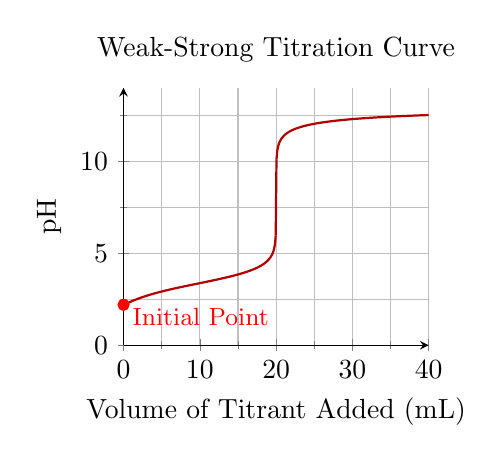
\begin{tikzpicture}[
        declare function={
            f(\x)= -log10(
                (sqrt(((\Mb*\x/(\Va+\x))+\ka)^2 + 4*\ka*((\Ma*\Va)-(\Mb*\x))/(\Va+\x)) - ((\Mb*\x/(\Va+\x))+\ka))/2
            );
            g(\x)=14+log10(
                (((\x*\Mb)-(\Va*\Ma))/(\Va+\x)) +
                (
                    sqrt(
                        ((((\x*\Mb)-(\Va*\Ma))/(\Va+\x)) + (10^(-14)/\ka))^2
                        + 4*(10^(-14)/\ka)*\Ma*\Va
                    )
                    - ((((\x*\Mb)-(\Va*\Ma))/(\Va+\x)) + (10^(-14)/\ka))
                )/2
            );
            h(\x)=14+log10(((sqrt(((10^(-14)/\ka)+10^(-7))^2 - 2 * \Ma * (10^(-14)/\ka))-((10^(-14)/\ka)+10^(-7)))/2)+10^(-7));
        }
    ]
        \pgfmathsetmacro{\ka}{0.00043}
        \pgfmathsetmacro{\Ma}{0.1}
        \pgfmathsetmacro{\Mb}{0.1}
        \pgfmathsetmacro{\Va}{20}
        \pgfmathsetmacro{\kb}{(10^(-14)/\ka)}
        \begin{axis}[
            xlabel={Volume of Titrant Added (mL)},
            ylabel={pH},
            title={Weak-Strong Titration Curve},
            grid=both,
            axis lines=left,
            minor tick num=1,
            width=0.45\textwidth,
            height=0.4\textwidth,
            ymin=0,
            ymax=14,
        ]
        % Add the titration curve
        \addplot[
            domain=0:{(\Va*\Ma/\Mb)-0.05},
            samples=200,
            thick,
            color=myred,
        ]{f(x)};
        \addplot[
            domain={(\Va*\Ma/\Mb)+0.05}:{2*\Va},
            samples=200,
            thick,
            color=myred,
        ]{g(x)};
        \addplot[mark=none, color=myred, thick] coordinates 
        {
            ({(\Va*\Ma/\Mb)-0.05}, {f(x)})
            ({(\Va*\Ma/\Mb)},{h(x)})
            ({(\Va*\Ma/\Mb)+0.05}, {g(x)})
            };
        \addplot[
                mark=*,
                only marks, 
                color=red, 
                nodes near coords, 
                point meta=explicit symbolic,
                nodes near coords style={below right, node font=\small, inner ysep=1pt},
                ] coordinates 
        {
            ({(\Va*\Ma/\Mb)}, {h(x)}) [Equivalence Point]
            ({0}, {f(0)}) [Initial Point]
        };
        \end{axis}
    \end{tikzpicture}
    \caption{A titration curve for a weak acid being titrated with a strong base.}
    \label{fig:titration_curve_weak}
\end{figure}

Figure \ref{fig:titration_curve_weak} shows a titration curve for a weak acid being titrated with a strong base. The initial point is at a higher pH than in the strong acid case, and has an initial hump before flattening out and then increasing rapidly at the equivalence point. 

\subsubsection{$pKa$ and Weak Acid/Base Titrations}

Similarly to pH, we can define $pK_a$ as the negative logarithm of the acid dissociation constant:
\begin{equation}\label{eq:pKa}
    pK_a = -\log K_a
\end{equation}
And we can define $pK_b$ as the negative logarithm of the base dissociation constant:
\begin{equation}\label{eq:pKb}
    pK_b = -\log K_b
\end{equation}
A nice property of $pK_a$ and $pK_b$ is that they are the pH values at which the concentrations of the acid and its conjugate base are equal, which is the point halfway between the starting point and the equivalence point on a titration curve. 

\subsubsection{Indicators}

\begin{figure}[h]
    \centering
    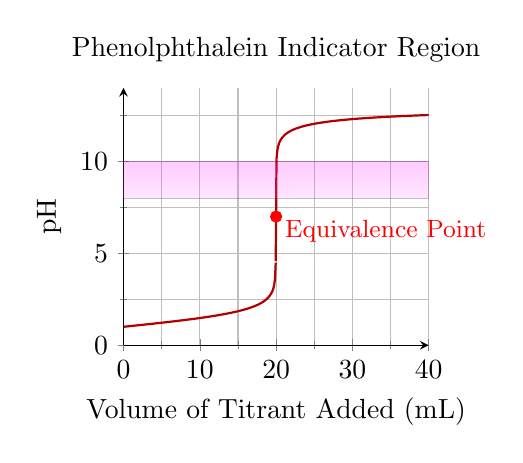
\begin{tikzpicture}[
        declare function={
            f(\x)= -log10(
                (sqrt(((\Mb*\x/(\Va+\x))+\ka)^2 + 4*\ka*((\Ma*\Va)-(\Mb*\x))/(\Va+\x)) - ((\Mb*\x/(\Va+\x))+\ka))/2
            );
            g(\x)=14+log10(
                (((\x*\Mb)-(\Va*\Ma))/(\Va+\x)) +
                (
                    sqrt(
                        ((((\x*\Mb)-(\Va*\Ma))/(\Va+\x)) + (10^(-14)/\ka))^2
                        + 4*(10^(-14)/\ka)*\Ma*\Va
                    )
                    - ((((\x*\Mb)-(\Va*\Ma))/(\Va+\x)) + (10^(-14)/\ka))
                )/2
            );
            h(\x)=14+log10(((sqrt(((10^(-14)/\ka)+10^(-7))^2 - 2 * \Ma * (10^(-14)/\ka))-((10^(-14)/\ka)+10^(-7)))/2)+10^(-7));
        }
    ]
        \pgfmathsetmacro{\ka}{13}
        \pgfmathsetmacro{\Ma}{0.1}
        \pgfmathsetmacro{\Mb}{0.1}
        \pgfmathsetmacro{\Va}{20}
        \pgfmathsetmacro{\kb}{(10^(-14)/\ka)}
        \begin{axis}[
            xlabel={Volume of Titrant Added (mL)},
            ylabel={pH},
            title={Phenolphthalein Indicator Region},
            grid=both,
            axis lines=left,
            minor tick num=1,
            width=0.45\textwidth,
            height=0.4\textwidth,
            ymin=0,
            ymax=14,
        ]
        % Add the titration curve
        \addplot[
            domain=0:{(\Va*\Ma/\Mb)-0.05},
            samples=200,
            thick,
            color=myred,
        ]{f(x)};
        \addplot[
            domain={(\Va*\Ma/\Mb)+0.05}:{2*\Va},
            samples=200,
            thick,
            color=myred,
        ]{g(x)};
        \addplot[mark=none, color=myred, thick] coordinates 
        {
            ({(\Va*\Ma/\Mb)-0.05}, {f(x)})
            ({(\Va*\Ma/\Mb)},{h(x)})
            ({(\Va*\Ma/\Mb)+0.05}, {g(x)})
            };
        \addplot[
                mark=*,
                only marks, 
                color=red, 
                nodes near coords, 
                point meta=explicit symbolic,
                nodes near coords style={below right, node font=\small, inner ysep=1pt},
                ] coordinates 
        {
            ({(\Va*\Ma/\Mb)}, {h(x)}) [Equivalence Point]
        };
        \draw[top color=magenta,bottom color=magenta!50!white, opacity=0.2] (0,8) rectangle (40,10);
        \end{axis}
    \end{tikzpicture}
    \caption{A titration curve with the region for color change of phenolphthalein highlighted.}
    \label{fig:titration_curve_indicator}
\end{figure}

When choosing an indicator for a titration, it is important to choose one that changes color around the pH of the equivalence point. In Figure \ref{fig:titration_curve_indicator}, phenolphthalein would be a good choice of indicator for this titration because it changes color in the pH range of 8.2 to 10, which is around the equivalence point of 7. Looking at the titration curve, we can see that the pH changes very rapidly around the equivalence point, so even if the endpoint is not exactly at the equivalence point, it will still be close enough for the indicator to change color.

Most indicators are weak acids or weak bases themselves, so they have their own equilibrium constants that determine the pH range over which they change color. For example, phenolphthalein is a weak acid with a $K_a$ of $5.0 \times 10^{-10}$, which corresponds to a pH range of 8.2 to 10 for its color change. The pH at which an indicator changes color is given by its $pK_a$. An indicator is a good choice for a titration if its $pK_a$ is close to the pH of the equivalence point of the titration.

\subsection{Solubility}
Solubility is the maximum amount of a substance that can dissolve in a given amount of solvent at a given temperature. The main factors that can affect how much of a substance can dissolve in a solvent is the pressure (if the solute is a gas), the amount of solvent, the specific substance, the temperature, the presence of other substances, the pH of the solution, and Amphoterism.
\subsubsection{The Solubility Product Constant}
The solubility product constant, $K_{sp}$, is the equilibrium constant for the dissolution of a salt in water. Given the reaction
\[\ce{A_nB_m_{(s)} <=> nA+_{(aq)} + mB-_{(aq)}}\]
the solubility product constant is given by the equation:
\begin{equation}\label{eq:Ksp}
    K_{sp} = [\ce{A+}]^n [\ce{B-}]^m
\end{equation}
The value of $K_{sp}$ can be used to determine the solubility of a salt in water. Given a salt \ce{A_nB_m} with a known value of $K_{sp}$, the amount of the salt that will dissolve in water can be calculated by setting up an equilibrium expression using the stoichiometry of the dissolution reaction and solving for the concentration of the ions in solution. The general form of this calculation is as follows:
\begin{equation}\label{eq:Ksp_general}
    K_{sp} = (nx)^n (mx)^m
\end{equation}
Where $x$ is some variable with the relation to the concentrations as follows:
\begin{align}
    [\ce{A+}] &= nx \label{eq:A_concentration}\\
    [\ce{B-}] &= mx \label{eq:B_concentration}
\end{align}
\subsubsection{The Common Ion Effect}
The common ion effect is the decrease in solubility of a salt when a common ion is added to the solution. To account for this effect, we use an ICE table with the initial concentration of the common ion included. This also applies to the dissociation of weak acids and weak bases, where the common ion is the conjugate base or conjugate acid, respectively. The presence of the common ion will shift the equilibrium position of the reaction, resulting in a decrease in the concentration of the ions in solution and therefore a decrease in solubility.
\subsection{Buffers}
A buffer is a solution that can resist changes in pH when small amounts of acid or base are added. Buffers are typically made from a weak acid and its conjugate base, or a weak base and its conjugate acid. The equilibrium between the weak acid and its conjugate base (or the weak base and its conjugate acid) allows the buffer to neutralize added acids or bases, thus maintaining a relatively constant pH. 

Buffers can be made by combining a weak acid and a weak base directly, or by using a salt of the weak acid or weak base with a common ion. 

A buffers capacity is the amount of acid or base that can be added to a buffer solution before a significant change in pH occurs. 

To calculate the pH of a buffer solution, we can use an ICE table with the initial concentrations of the weak acid and its conjugate base (or the weak base and its conjugate acid) included. We can then set up an equilibrium expression using the stoichiometry of the reaction and solve for the concentration of hydrogen ions in solution, which can then be used to calculate the pH of the buffer solution.

Another way to calculate the pH of a buffer solution is to use the Henderson-Hasselbalch equation, which is derived from the equilibrium expression for the dissociation of a weak acid or weak base. The Henderson-Hasselbalch equation is given by:
\begin{equation}\label{eq:Henderson_Hasselbalch_pH}
    \text{pH} = pK_a + \log \left( \frac{[\text{A-}]}{[\text{HA}]} \right)
\end{equation}

This equation can be used to estimate the pH of a buffer solution if the concentrations of the weak acid and its conjugate base (or the weak base and its conjugate acid) are known, as well as the $pK_a$ of the weak acid (or the $pK_b$ of the weak base). It is important to note that the Henderson-Hasselbalch equation is only an approximation and is most accurate when the concentrations of the weak acid and its conjugate base (or the weak base and its conjugate acid) are similar.

The equation for a weak base buffer solution is similar, but uses $pK_b$ instead of $pK_a$ and the concentrations of the weak base and its conjugate acid instead of the weak acid and its conjugate base:
\begin{equation}\label{eq:Henderson_Hasselbalch_pOH}
    \text{pOH} = pK_b + \log \left( \frac{[\text{BH+}]}{[\text{B}]} \right)
\end{equation}
This equation also shows us that the pH of a buffer solution made up of equal parts of a weak acid and its conjugate base will be equal to the $pK_a$ of the weak acid. This is because when the concentrations of the weak acid and its conjugate base are equal, the ratio in the logarithm is equal to 1, and $\log(1) = 0$, so the equation simplifies to $\text{pH} = pK_a$.


\section{Thermodynamics}
Thermodynamics is the study of energy and its transformations. In chemistry, it is used to understand the energy changes that occur during chemical reactions and physical processes. At it's core energy is the ability to do work or produce heat. There are two main types of energy: kinetic energy, which is the energy of motion, and potential energy, which is the energy stored in an object due to its position or configuration. The total energy of a system is the sum of its kinetic and potential energy. 

Kinetic energy is given by the equation \eqref{eq:KE}, and includes subtypes of energy such as thermal, mechanical, and electrical energy. Potential energy includes chemical energy, which is stored in the bonds of molecules, and nuclear energy, which is stored in the nucleus of an atom. The force between two charged particles is given by Coulomb's Law, which is expressed in equation \eqref{eq:coulombs} is also a form of potential energy. 

\subsection{Properties of Energy}
\subsubsection{Laws of Thermodynamics}
Energy is governed by three main laws called the laws of thermodynamics. 

The first law of thermodynamics, also known as the law of energy conservation, states that energy cannot be created or destroyed, only transferred or transformed. This means that the total energy of an isolated system remains constant. This can be mathematically expressed as:
\begin{equation}\label{eq:firstLaw}
    \Delta H_\text{System} + \Delta H_\text{Surroundings} = 0
\end{equation}
Where $\Delta H$ is the change in enthalpy (see section \ref{sec:enthalpy}). 

The second law of thermodynamics states that the total entropy of an isolated system can never decrease over time. This means that natural processes tend to move towards a state of greater disorder or randomness. See section \ref{sec:entropy} for more information on entropy.

The third law of thermodynamics states that as the temperature of a system approaches absolute zero, the entropy of the system approaches a minimum value. This means that at absolute zero, the system is in a state of perfect order and has zero entropy. This law also implies that it is impossible to reach absolute zero in a finite number of steps, and that as temperature decreases, the efficiency of energy transfer processes increases.
\subsubsection{Heat, Temperature, Work, and Power}
Temperature is a measure of the average kinetic energy of the particles in a substance. We measure temperature in degrees Celsius (\textdegree C) or Kelvin (K). A high temperature means a high average kinetic energy, while a low temperature means a low average kinetic energy. 

Heat is the transfer of energy from one object to another due to a temperature difference. Heat flows from a hotter object to a cooler object until thermal equilibrium is reached. For most cases in chemistry, heat can be represented by the change in enthalpy $\Delta H$ of a system, which is the heat absorbed or released during a chemical reaction or physical process.

Work is the transfer of energy that occurs when a force is applied to an object and causes it to move. This is not as common in chemistry and is mostly found in physics, but the equation for work is given by:
\begin{equation}\label{eq:work}
    W = F \Delta x
\end{equation}
Where $F$ is the force applied and $\Delta x$ is the distance moved. A Force is just a push or pull and can be related to acceleration by Newton's second law,
\begin{equation}\label{eq:newton}
    F = ma
\end{equation}
Where $m$ is the mass of the object and $a$ is the acceleration. Power is the rate at which work is done or energy is transferred. It is measured in watts (W) and is given by the equation:
\begin{equation}\label{eq:power}
    P = \frac{W}{t}
\end{equation}
Where $W$ is the work done and $t$ is the time taken to do the work. 
\subsection{Enthalpy, Entropy, and Free Energy}
\subsubsection{Enthalpy}\label{sec:enthalpy}
Enthalpy ($H$) is a measure of the total energy of a system, including both kinetic and potential energy. Usually we are interested in the change in enthalpy expressed as $\Delta H$, which is the difference in enthalpy at the end of a process and the beginning of a process. The change in enthalpy can be found using the heat equation:
\begin{equation}\label{eq:heat}
    \Delta H = mC\Delta T
\end{equation}
Where $m$ is the mass of the substance, $C$ is the specific heat capacity, and $\Delta T$ is the change in temperature. This equation can be used to calculate the heat or change in enthalpy for a substance when it is heated or cooled.
The specific heat capacity ($C$) is the amount of heat required to raise the temperature of one gram of a substance by one degree Celsius. It is a physical property of a substance and is independent on the amount of substance present. The specific heat capacity is different for different phases of matter, with solids generally having lower specific heat capacities than liquids and gases. 
\subsubsection{Entropy}\label{sec:entropy}
Entropy ($S$) is a measure of the disorder or randomness of a system. The equation for entropy is given by:
\begin{equation}\label{eq:entropy}
    S = k \ln{W}
\end{equation}
Where $k$ is Boltzmann's constant and $W$ is the number of microstates available to the system. A microstate is a specific arrangement of particles in a system, and the more microstates available, the higher the entropy. The change in entropy ($\Delta S$) can be calculated using the equation:
\begin{equation}\label{eq:deltaS}
    \Delta S_\text{System} = \frac{\Delta H_\text{System}}{T}
\end{equation}
Where $\Delta H_\text{System}$ is the change in enthalpy of the system and $T$ is the temperature in Kelvin. This equation shows that the change in entropy is directly proportional to the change in enthalpy and inversely proportional to the temperature. The second law of thermodynamics states that the total entropy of an isolated system can never decrease over time, which means that natural processes tend to move towards a state of greater disorder or randomness. This implies that spontaneous processes are those that increase the total entropy of the system and its surroundings.
A process is spontaneous if it occurs without the input of external energy. 

When a substance undergoes a phase change, such as from solid to liquid or from liquid to gas, there is a change in entropy. This is because the particles in the substance become more disordered as they move from a more ordered phase (solid) to a less ordered phase (liquid) and then to an even less ordered phase (gas). 

The entropy of atoms and molecules is related to their degrees of freedom, which are the ways in which they can move and rotate. For example, a diatomic molecule has more degrees of freedom than a monatomic atom, and therefore has a higher entropy. The more bonds a molecule has, the more ways it can rotate and flex and therefore the higher its entropy. Additionally, larger molecules generally have higher entropy than smaller molecules because they have more atoms and therefore more degrees of freedom.

The entropy change of a chemical reaction will increase the more gas molecules are produces, the more molecules are involved, the higher the phase energy, the more mixed the products are, and the larger the temperature increase since faster molecules are more chaotic. 
\subsubsection{Gibbs Free Energy}
The amount of energy available to do work in a system is called the Gibbs free energy ($G$). The change in Gibbs free energy ($\Delta G$) can be calculated using the equation:
\begin{equation}\label{eq:free_energy}
    \Delta G = \Delta H - T\Delta S
\end{equation}
Where $\Delta H$ is the change in enthalpy, $T$ is the temperature in Kelvin, and $\Delta S$ is the change in entropy. A negative value of $\Delta G$ indicates that a process is spontaneous, while a positive value indicates that a process is non-spontaneous. If $\Delta G$ is zero, the system is at equilibrium. Using this equation, we can determine whether a reaction is spontaneous or not under certain conditions. 
\begin{table}[ht]
    \centering
    \begin{tabular}{c c c}
        $\Delta H$ & $\Delta S$ & Spontaneity \\
        \hline
        $-$ & $+$ & Spontaneous \\
        $-$ & $-$ & Spontaneous for small $T$ \\
        $+$ & $+$ & Spontaneous for large $T$ \\
        $+$ & $-$ & Non-Spontaneous \\
    \end{tabular}
    \caption{Spontaneity of Reactions Based on Enthalpy and Entropy Changes}
    \label{table:spontaneity}
\end{table}
Looking at table \ref{table:spontaneity}, we can see when a reaction will be spontaneous based on the signs of $\Delta H$ and $\Delta S$. 
\subsection{Calorimetry}
Calorimetry is the measurement of heat transfer during a chemical reaction or physical process. It is used to determine the enthalpy change or heat of a reaction. This is mostly accomplished using a calorimeter, which is an insulated container that minimizes heat exchange with the surroundings. By measuring the temperature change of the system and knowing the specific heat capacity and mass of the substance, we can calculate the heat transfer using the heat equation \eqref{eq:heat}.
\subsubsection{System and Surroundings}
In calorimetry, the system is the part of the universe that is being studied, while the surroundings are everything else. The system can be an object, a chemical reaction, or a physical process. The surroundings can include the container, the air, and any other objects that are not part of the system. There are three types of systems: open, closed, and isolated. An open system can exchange both matter and energy with its surroundings, a closed system can exchange only energy, and an isolated system cannot exchange either matter or energy.
\subsubsection{Exothermic and Endothermic}
A process is exothermic if it releases heat to the surroundings, which means that $\Delta H$ is negative. A process is endothermic if it absorbs heat from the surroundings, which means that $\Delta H$ is positive. 
\subsubsection{Phase Changes}
Energy is required to change the phase of a substance, such as from solid to liquid or from liquid to gas. The amount of energy required for a phase change is called the heat of fusion (for melting) or the heat of vaporization (for boiling). These values can be used to calculate the heat transfer during a phase change using the equation:
\begin{equation}\label{eq:phase_change}
    \Delta H = n\Delta H_\text{phase change}
\end{equation}
Where $n$ is the number of moles of the substance and $\Delta H_\text{phase change}$ is the heat of fusion or vaporization. When a substance undergoes a phase change, the temperature remains constant until the phase change is complete, even though heat is being transferred. This is because the energy is being used to break or form intermolecular forces rather than to increase the kinetic energy of the particles. The heat of fusion, heat of vaporization, and specific heat capacities of water can be found below in table \ref{table:water_properties}.
\begin{table}[ht]
    \centering
    \begin{tabular}{l c}
        Property & Value \\
        \hline
        $C_l$ & 4.184 J/g\textdegree C \\
        $C_s$ & 2.05 J/g\textdegree C \\
        $C_g$ & 1.996 J/g\textdegree C \\
        $\Delta H_\text{fus}$ & 6.01 kJ/mol or 334 J/g \\
        $\Delta H_\text{vap}$ & 40.7 kJ/mol or 2260 J/g \\
    \end{tabular}
    \caption{Thermodynamic Properties of Water}
    \label{table:water_properties}
\end{table}
\begin{figure}[ht]
    \centering
    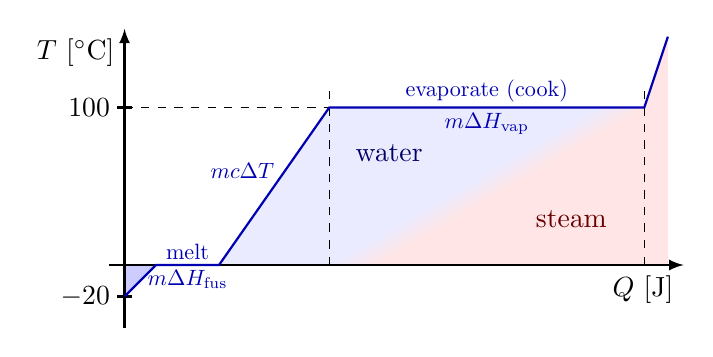
\begin{tikzpicture}
        \message{Phase transition of ice -> water -> steam^^J}
        \def\ymin{-0.8}
        \def\ymax{3}
        \def\xmin{-0.2}
        \def\xmax{7}
        \def\t{0.3}    % water/steam transition zone
        \def\ang{30.4} % angle gradient
        \coordinate (O) at (0,0);
        \coordinate (I) at (0.0,-0.4); % ice
        \coordinate (M) at (0.4,0.0);  % melting
        \coordinate (W) at (1.2,0.0);  % water
        \coordinate (E) at (2.6,2,0);  % evaporate
        \coordinate (S) at (6.6,2.0);  % steam
        \coordinate (F) at (6.9,2.9);  % final
        \coordinate (Ex) at ($(E|-O)$); % x evaporation
        \coordinate (Ey) at ($(E-|O)$); % y evaporation
        \coordinate (Sx) at ($(S|-O)$); % x steam
        \coordinate (Fx) at ($(F|-O)$);
        
        % AREA
        \fill[mylightblue] (O) -- (I) -- (M) -- cycle;
        \fill[blue!8] (W) -- (Ex) -- (S) -- (E) -- cycle;
        \fill[mylightred] (Ex) -- (S) -- (F) -- (Fx) -- cycle;
        \begin{scope} % fade/gradient border
            \clip (Ex) -- (Sx) -- (S) -- (E) -- cycle; % clip gradient rectangle
            \draw[draw=none,transform canvas={rotate=\ang},top color=blue!8,bottom color=mylightred,shading angle=0]
            ({2.6*cos(\ang)},{-2.6*sin(\ang)-\t}) rectangle++(0.65*\xmax,\t); % diagonal border 
        \end{scope}
        \node[blue!40!black,left=4,below right=10] at (E) {water};
        \node[red!40!black,above left=10] at (Sx) {steam};
        
        % AXES
        \draw[->,thick] (0,\ymin) -- (0,\ymax) node[below left=0] {$T$ [\si{\degree C}]};
        \draw[->,thick] (\xmin,0) -- (\xmax+0.1,0) node[below left=0] {$Q$ [J]}; %[\si{J}]
        \draw[dashed] (Ex) -- (E) --++ (0,0.1*\ymax);
        \draw[dashed] (Ey) -- (E);
        \draw[dashed] (Sx) -- (S) --++ (0,0.1*\ymax);
        \tick{I}{0} node[left=-1] {$-20$};
        \tick{Ey}{0} node[left=-1] {$100$};
        
        \draw[dashed] (E) -- (Ex);
        \draw[myblue,thick]
            (I) -- (M) -- (W)
            node[midway,above=-1,scale=0.8] {melt}
            node[midway,below=-1,scale=0.8] {$m\Delta H_\mathrm{fus}$} --
            (E)
            node[pos=0.6,left=1,scale=0.8] {$mc\Delta T$} --
            (S)
            node[midway,above=-1,scale=0.8] {evaporate (cook)}
            node[midway,below=-1,scale=0.8] {$m\Delta H_\mathrm{vap}$} --
            (F);
        
        \end{tikzpicture}
    \caption{Heating curve of water.}
    \label{fig:heating_curve}
\end{figure}
\subsubsection{Enthalpy of Reaction and Molar Heat}
The enthalpy of reaction ($\Delta H_\text{rxn}$) is the change in enthalpy that occurs during a chemical reaction. Similarly, the molar heat of a reaction is the enthalpy change per mole of a substance involved in the reaction. It can be calculated by dividing the enthalpy change by the number of moles of the substance. These values can be used to convert between the amount of heat transferred and the amount of substance involved in a reaction using stoichiometry.

\subsection{Light Waves and their Energies}
Electromagnetic radiation, or light, is a form of energy that travels in waves. The energy of a light wave is directly proportional to its frequency ($\nu$) and inversely proportional to its wavelength ($\lambda$). The frequency and wavelength of light are related by the equation:
\begin{equation}\label{eq:light_speed}
    c = \lambda \nu
\end{equation}
Where $c$ is the speed of light, which is approximately $3.00 \times 10^8$ m/s. The energy of a light wave can be calculated using the equation:
\begin{equation}\label{eq:light_energy}
    E = h\nu = \frac{hc}{\lambda}
\end{equation}
Where $h$ is Planck's constant, which is approximately $6.626 \times 10^{-34}$ J·s. This equation shows that the energy of a photon is proportional to its frequency and inversely proportional to its wavelength. This means that higher frequency light (such as ultraviolet) has more energy than lower frequency light (such as infrared).
The electromagnetic spectrum is the range of all types of electromagnetic radiation, which includes radio waves, microwaves, infrared, visible light, ultraviolet, X-rays, and gamma rays. Each type of radiation has a different wavelength and frequency, and therefore a different energy. Each different wavelength of light corresponds to a different color in the visible spectrum, with red having the longest wavelength around 650 nm, Orange around 590 nm, Yellow around 570 nm, Green around 510 nm, Blue around 475 nm, and Violet around 400 nm. 
In addition the energies of photons can be used to determine their mass using the equation:
\begin{equation}\label{eq:massEnergy}
    E = mc^2
\end{equation}
Where $m$ is the mass of the photon and $c$ is the speed of light. 

Photons can cause electrons to be excited to higher energy levels, which causes them to emit light when they return to their ground state. This is the basis for phenomena such as fluorescence and phosphorescence. The energy of the emitted light corresponds to the difference in energy between the excited state and the ground state. For more see section \ref{sec:atomModels}.

\subsection{Enthalpy, Entropy, and Free Energy of Reactions}
\subsection{Standard Conditions and Standard State}
Standard conditions refer to a set of specific conditions that are used as a reference point for measuring and comparing the properties of substances and reactions. The standard state of a substance is its most stable form at a pressure of 1 atm, a temperature of 25\textdegree C (298.15 K), a concentration of 1 M for solutions, and a pH of 7 for aqueous solutions. The standard enthalpy change ($\Delta H^\circ$), standard entropy change ($\Delta S^\circ$), and standard Gibbs free energy change ($\Delta G^\circ$) of a reaction are the changes in these properties when the reactants and products are in their standard states. The circle, called naught, in each of these symbols indicates that the values are measured under standard conditions. 
\subsection{Enthalpy of Formation}
The enthalpy of formation ($\Delta H_f^\circ$) is the change in enthalpy that occurs when one mole of a compound is formed from its elements in their standard states. The standard enthalpy of formation for an element in its most stable form is defined as zero. The enthalpy change of a reaction can be calculated using the enthalpies of formation of the reactants and products using the equation:
\begin{equation}\label{eq:enthalpy_of_formation}
    \Delta H_\text{rxn} = \sum \Delta H_f^\circ(\text{prod}) - \sum \Delta H_f^\circ (\text{react})
\end{equation}
This equation allows us to calculate the enthalpy change of a reaction using tabulated values of the enthalpies of formation of the substances involved in the reaction.
\subsection{Entropy of Formation}
The entropy of formation ($\Delta S_f^\circ$) is the change in entropy that occurs when one mole of a compound is formed from its elements in their standard states. Similar to the enthalpy of formation, the standard entropy of formation for an element in its most stable form is defined as zero. The entropy change of a reaction can be calculated using the entropies of formation of the reactants and products using the equation:
\begin{equation}\label{eq:entropy_of_formation}
    \Delta S_\text{rxn} = \sum \Delta S_f^\circ(\text{prod}) - \sum \Delta S_f^\circ (\text{react})
\end{equation}
This is the same as the equation for enthalpy of formation, but with entropy values instead.
\subsection{Gibbs Free Energy of Formation}
The Gibbs free energy of formation ($\Delta G_f^\circ$) is the change in Gibbs free energy that occurs when one mole of a compound is formed from its elements in their standard states. Similar to the enthalpy and entropy of formation, the standard Gibbs free energy of formation for an element in its most stable form is defined as zero. The Gibbs free energy change of a reaction can be calculated using the Gibbs free energies of formation of the reactants and products using the equation:
\begin{equation}\label{eq:free_energy_of_formation}
    \Delta G_\text{rxn} = \sum \Delta G_f^\circ(\text{prod}) - \sum \Delta G_f^\circ (\text{react})
\end{equation}
This is the same as the equations for enthalpy and entropy of formation, but with Gibbs free energy values instead. 
In addition to calculating the Gibbs free energy change of a reaction, we can also use the standard Gibbs free energy of formation to calculate the equilibrium constant ($K$) of a reaction using the equation:
\begin{equation}\label{eq:free_energy_equilibrium}
    \Delta G^\circ = -RT \ln{K}
\end{equation}
Where $R$ is the gas constant and $T$ is the temperature in Kelvin. This equation showcases the relationship between the Gibbs free energy change of a reaction and its equilibrium constant. In addition, we can write out how the Gibbs free energy change of a reaction changes with different concentrations of reactants and products using the equation:
\begin{equation}\label{eq:free_energy_concentration}
    \Delta G = \Delta G^\circ + RT \ln{Q}
\end{equation}
Where $Q$ is the reaction quotient, which is the ratio of the concentrations of products to reactants at any given point in time. 
\section{Electrochemistry}
Electrochemistry is the study of the chemical processes that involve the movement of electrons. It encompasses a wide range of phenomena, including redox reactions, electrolysis, and the operation of batteries. Before diving into the specifics of electrochemistry, it is recommended to review the concepts of oxidation and reduction from section \ref{sec:OxidationReduction}.
\subsection{Galvanic/Voltaic Cells}
A galvanic cell, also known as a voltaic cell, is a device which harnesses the energy released from a spontaneous redox reaction to generate an electric current. It consists of two half-cells, each containing an electrode and an electrolyte solution. The half-cells are connected by a salt bridge, which allows ions to flow between them while preventing the mixing of the different solutions. The two electrodes are then connected by a wire, allowing electrons to flow from the anode (where oxidation occurs) to the cathode (where reduction occurs). The number of electrons flowing through the wire per unit time is the electric current, which can be measured in amperes (A). The formula for calculating the electric current is:
\begin{equation}\label{eq:Current}
I = \frac{Q}{t}
\end{equation}
where $I$ is the current, $Q$ is the charge in coulombs (C), and $t$ is the time in seconds (s). In addition the voltage (or electromotive force, EMF) of the cell is the potential difference between the two electrodes, which is relatable to how height is the potential for an object to fall. Voltage can be calculated from energy and charge using the formula:
\begin{equation}\label{eq:Voltage}
V = \frac{E}{Q}
\end{equation}
where $V$ is the voltage in volts (V), $E$ is the energy in joules (J), and $Q$ is the charge in coulombs (C). The resistance of the circuit is the opposition to the flow of electric current, and it can be calculated using Ohm's law:
\begin{equation}\label{eq:Resistance}
    R = \frac{V}{I}
\end{equation}
where $R$ is the resistance in ohms ($\Omega$). 
\begin{figure}[ht]
    \centering
    \includegraphics[width=0.4\textwidth]{Screenshot 2026-06-03 at 9.09.06 PM.png}
    \caption{Schematic of a galvanic cell}
    \label{fig:GalvanicCell}
\end{figure}
In figure \ref{fig:GalvanicCell}, the porous disk is equivalent to the salt bridge, which allows ions to flow between the two half-cells while preventing the mixing of the different solutions. As the reaction proceeds, the anode will lose mass as it is oxidized, its metal becoming ions dissolved in the solution, while the cathode will gain mass as it is reduced, its ions from the solution plating onto the electrode. A mnemonic for remembering the direction of electron flow is ``An Ox gets thin, while the Red Cat gets fat'' (Anode Oxidation, Reduction Cathode).
\subsubsection{Line Notation}
Line notation is a shorthand way of representing the components of a galvanic cell. It is written in the form:
\[\text{Anode} | \text{Anode Solution} || \text{Cathode Solution} | \text{Cathode}\]

where the single vertical line (|) represents a phase boundary, and the double vertical line (||) represents the salt bridge. For example the line notation 
\[\ce{Mg(s) | Mg^{2+}(aq) || Al^{3+}(aq) | Al(s)}\]
represents the reaction,
\[\ce{3Mg(s) + 2Al^{3+}(aq) -> 3Mg^{2+}(aq) + 2Al(s)}\]
\subsection{Electromotive Force (EMF)}
The electromotive force ($\mathcal{E}$) is the difference in electrical potential between the two electrodes of a galvanic cell. It is measured in volts (V) and can be calculated using the standard reduction potentials of the half-reactions occurring at the anode and cathode. The formula for calculating the EMF of a galvanic cell is:
\begin{equation}\label{eq:EMF}
\mathcal{E} = E^\circ_{\text{cathode}} - E^\circ_{\text{anode}}
\end{equation}
where $E^\circ_{\text{cathode}}$ is the standard reduction potential of the cathode and $E^\circ_{\text{anode}}$ is the standard reduction potential of the anode. The standard reduction potentials can be found in tables, such as table \ref{table:StandardPotential}. A positive EMF indicates a spontaneous reaction, while a negative EMF indicates a non-spontaneous reaction. 
\subsubsection{The Activity Series}
The activity series is a list of elements ranked in order of their ability to be oxidized. It is used to predict the outcome of redox reactions, particularly single displacement reactions. The activity series is based on the standard reduction potentials of the elements, with those having more negative potentials being more easily oxidized. 
\subsubsection{$\mathcal{E}$, $\Delta G$, and the Nernst Equation}
The relationship between the electromotive force ($\mathcal{E}$) of a galvanic cell and the Gibbs free energy change ($\Delta G$) of the reaction can be expressed by the following equation:
\begin{equation}\label{eq:EMF_DeltaG}
\Delta G = -nF\mathcal{E}
\end{equation}
where $n$ is the number of moles of electrons transferred in the reaction, and $F$ is the Faraday constant, approximately equal to 96485 C/mol. This equation indicates that a positive EMF corresponds to a negative $\Delta G$, which means the reaction is spontaneous, while a negative EMF corresponds to a positive $\Delta G$, indicating a non-spontaneous reaction. 

This is further related to the Nernst equation, which allows for the calculation of the EMF of a cell under non-standard conditions:
\begin{equation}\label{eq:Nernst}
\mathcal{E} = \mathcal{E}^\circ - \frac{RT}{nF} \ln Q
\end{equation}
where $\mathcal{E}^\circ$ is the standard EMF, $R$ is the ideal gas constant (8.314 J/mol$\cdot$K), $T$ is the temperature in Kelvin, $n$ is the number of moles of electrons transferred, $F$ is the Faraday constant, and $Q$ is the reaction quotient. The Nernst equation is no longer required for the AP exam, but it is a useful tool and can be applied to some problems.
\subsection{Electrolytic Cells}
An electrolytic cell is very similar to a galvanic cell, but it requires an external source of electrical energy to drive a non-spontaneous reaction. With this we can do things like electrolysis or electroplating.
\subsubsection{Electrolysis}
Electrolysis is the process of using an electric current to drive a non-spontaneous chemical reaction. It is commonly used for the decomposition of compounds, such as the electrolysis of water to produce hydrogen and oxygen gas:
\[\ce{2H2O(l) -> 2H2(g) + O2(g)}\]
To do math with electrolysis, just remember that amps are coulombs per second (equation \eqref{eq:Current}), and that 1 mole of electrons is 96485 coulombs (Faraday's constant). Using this values you can use stoichiometry to find the amount of product produced or reactant consumed in an electrolysis reaction. 
\subsubsection{Electroplating}
Electroplating is the process of using electrolysis to deposit a thin layer of metal onto a surface. This is a type of electrolysis where the cathode is the object being plated, and the anode is a piece of the metal being deposited. 
\section{AP Atom}
\subsection{Atomic Theory and Quantum Mechanics}
\subsubsection{Models of the Atom}\label{sec:atomModels}
The first main atomic theory was proposed by John Dalton in the early 19th century, which described atoms as indivisible particles. He came up with 4 main laws of atomic theory:
\begin{itemize}
    \item All matter is made of atoms, which are indivisible and indestructible.
    \item All atoms of a given element are identical in mass and properties.
    \item Atoms of one element can not be changed into atoms of another element by chemical reactions, and they can not be created or destroyed in chemical reactions.
    \item Compounds are formed when atoms of different elements combine in fixed ratios.
\end{itemize}
This was then improved upon by J.J. Thomson, who discovered the electron and proposed the "plum pudding" model of the atom, where electrons were embedded in a positively charged "pudding". However, this model was disproven by Ernest Rutherford's gold foil experiment, which led to the nuclear model of the atom, where a small, dense nucleus is surrounded by electrons.

It was later refined by Niels Böhr, who proposed that electrons orbit the nucleus in specific energy levels or shells. This model explained the discrete spectral lines of hydrogen but failed to account for more complex atoms. The model he proposed left him with more questions than answers, such as why electrons do not spiral into the nucleus and how to explain the spectra of atoms with more than one electron.

The model Böhr proposed had several planet like orbits at specific energy levels for the electrons. Each one of these energy levels was given a quantum number $n$, and electrons could jump between these energy levels by absorbing or emitting photons of specific energies. The equation he came up to describe this was:
\begin{equation}\label{eq:bohr}
    E_n = -2.178 \times 10^{-18} \frac{Z^2}{n^2} \text{ J}
\end{equation}
where $E_n$ is the energy of the electron at a specific energy level, $Z$ is the atomic number, and $n$ is the principal quantum number. This equation successfully explained the spectral lines of hydrogen but could not account for more complex atoms or the behavior of electrons in multi-electron systems.

De Broglie hypothesized that particles, such as electrons, could exhibit wave-like properties. He proposed that the wavelength of a particle is inversely proportional to its momentum, given by the equation:
\begin{equation}\label{eq:debroglie}
    \lambda = \frac{h}{mv}
\end{equation}
where $\lambda$ is the wavelength, $h$ is Planck's constant, $m$ is the mass of the particle, and $v$ is its velocity.

It was then found that electron beams exhibited wave-like properties, specifically diffraction and interference patterns. The photoelectric effect, observed by Albert Einstein, provided evidence for the quantization of energy and the particle-like nature of light. Only certain energy levels are allowed for electrons in an atom, and electrons can transition between these levels by absorbing or emitting photons of specific energies. This explains the discrete spectral lines observed in atomic spectra.

Heisenberg then presented his uncertainty principle, which states that it is impossible to simultaneously know both the exact position and momentum of a particle. This is expressed mathematically as:
\begin{equation}\label{eq:heisenberg}
    \Delta x \Delta p \geq \frac{h}{4\pi}
\end{equation}
where $\Delta x$ is the uncertainty in position and $\Delta p$ is the uncertainty in momentum. 

The culmination of these discoveries led to the development of quantum mechanics, which provides a more comprehensive and accurate description of atomic and subatomic phenomena. The Schrödinger equation, a fundamental equation in quantum mechanics, describes how the quantum state of a physical system changes over time. It is given by:
\begin{equation}\label{eq:schrodinger}
    i\hbar \frac{\partial}{\partial t} \Psi(\mathbf{r}, t) = \hat{H} \Psi(\mathbf{r}, t)
\end{equation}
You do not need to know the structure of the Schrödinger equation, but it is important to understand the implications of quantum mechanics.
\subsubsection{Quantum Numbers}
What the equation tells us is that there is a principal quantum number $n$ that describes the energy level of an electron in an atom. In addition there is an orbital quantum number $l$ that describes the shape of the orbital, a magnetic quantum number $m_l$ that describes the orientation of the orbital in space, and a spin quantum number $m_s$ that describes the intrinsic angular momentum of the electron. The values of these numbers are as follows:
\begin{itemize}
    \item $n\in\mathbb{N}\quad(1,2,3,\dots)$
    \item $0 \le l < n$
    \item $-l \le m_l \le l$
    \item $m_s$ can be either +1/2 or -1/2
\end{itemize}
\subsubsection{Electron Configuration}
Electrons fill orbitals in a specific order based on their energy levels, following the Pauli exclusion principle, Hund's rule, and the Aufbau principle. The Pauli exclusion principle states that no two electrons can have the same set of quantum numbers, meaning that an orbital can hold a maximum of two electrons with opposite spins. Hund's rule states that electrons will fill degenerate orbitals (orbitals with the same energy) singly before pairing up. The Aufbau principle states that electrons occupy the lowest energy orbitals first. This leads to the electron configuration of atoms, which describes the distribution of electrons in the various orbitals. We write the electron configuration of an atom using the notation $n\ell^x$, where $n$ is the principal quantum number, $\ell$ is the type of orbital (s, p, d, f), and $x$ is the number of electrons in that orbital. For example, the electron configuration of carbon (atomic number 6) is $1s^2 2s^2 2p^2$, which means it has 2 electrons in the 1s orbital, 2 electrons in the 2s orbital, and 2 electrons in the 2p orbital.

An excited state of an atom occurs when one or more electrons are promoted to higher energy levels than their ground state configuration. This can happen when an atom absorbs energy, such as from heat or light. For example, if a carbon atom absorbs energy, one of its 2s electrons could be promoted to the 2p orbital, resulting in an excited state with the configuration $1s^2 2s^1 2p^3$. Excited states are typically unstable and will eventually return to the ground state by emitting energy in the form of photons.

Sometimes the electron configuration may be written in a condensed form using the noble gas notation. This involves using the symbol of the nearest noble gas that comes before the element in the periodic table to represent the inner electron configuration. For example, the electron configuration of sodium (atomic number 11) can be written as $[Ne] 3s^1$, where $[Ne]$ represents the electron configuration of neon ($1s^2 2s^2 2p^6$). This notation is often used to simplify the representation of electron configurations for elements with many electrons.

There are two weird exceptions to the expected electron configurations based. A filled $3d$ subshell is more stable than a filled $4s$ subshell, and the $xf^1$ configuration is more stable than the $x-1d^9$ configuration. This means that for elements like chromium (atomic number 24) and copper (atomic number 29), the expected electron configurations would be $[Ar] 4s^2 3d^4$ and $[Ar] 4s^2 3d^9$, respectively. However, due to the increased stability of a filled $3d$ subshell, the actual electron configurations are $[Ar] 4s^1 3d^5$ for chromium and $[Ar] 4s^1 3d^{10}$ for copper.

When writing the electron configuration of an ion, we need to account for the loss or gain of electrons. For cations (positively charged ions), we remove electrons starting from the highest energy level. This is not necessarily the last orbital filled, but rather the orbital with the highest principal quantum number. Anions (negatively charged ions) gain electrons, and we add electrons to the next available orbital following the same order as for neutral atoms. 
\subsection{The Periodic Table}
\subsubsection{Organization}
The periodic table is organized into three main groups: metals, nonmetals, and metalloids. Metals are typically found on the left side and center of the periodic table, while nonmetals are located on the right side. Metalloids have properties that are intermediate between metals and nonmetals and are found along the zigzag line that separates metals and nonmetals.

There are several families of elements in the periodic table, including alkali metals (Group 1), alkaline earth metals (Group 2), transition metals (Groups 3-12), halogens (Group 17), and noble gases (Group 18). Each family has distinct properties and trends in their chemical behavior.
\subsubsection{Metals vs Nonmetals}
Metals have very high attractive forces between their individual atoms, which results in their electrons being demoralized and free to move throughout the metal lattice. The effect of this is that metals are good conductors of electricity and heat. Metals are also malleable and ductile, meaning they can be hammered into thin sheets or drawn into wires without breaking. They also have high melting and boiling points due to the strong metallic bonds between atoms. They tend to form positive ions (cations) by losing electrons in reactions.

Nonmetals, on the other hand, have weaker attractive forces between their atoms, which results in their electrons being more localized and less free to move. This makes nonmetals poor conductors of electricity and heat. Nonmetals are also brittle and tend to break rather than deform when subjected to stress. They generally have lower melting and boiling points compared to metals. Nonmetals tend to form negative ions (anions) by gaining electrons in reactions.
\subsubsection{Effective Nuclear Charge}
All the periodic trends are based on the electron's attraction to the nucleus. Every electron is independently attracted to the nucleus, but they are also repelled by other electrons. The effective nuclear charge ($Z_{\text{eff}}$) is the net positive charge experienced by an electron in a multi-electron atom. It can be calculated using the formula:
\begin{equation}\label{eq:zeff}
    Z_{\text{eff}} = Z - S
\end{equation}
where $Z$ is the atomic number and $S$ is the shielding constant. Usually, the shielding constant will be approximately equal to the number of inner electrons, as they are more effective at shielding the outer electrons from the nucleus. It is possible that some AP tests will ask you to use other conventions for calculating the shielding constant, such as assigning different values for electrons in different orbitals. 
\subsubsection{Periodic Trends}
Atomic radius or bonding radius is half the distance between two bound atoms. As you move down a group in the periodic table, the atomic radius increases due to the addition of electron shells while the effective nuclear charge remains relatively constant. As you move across a period from left to right, the atomic radius decreases because the effective nuclear charge increases, pulling the electrons closer to the nucleus.

Ionization energy is the energy required to remove an electron from an atom. As you move down a group, ionization energy decreases because the outer electrons are farther from the nucleus and are more shielded by inner electrons. As you move across a period from left to right, ionization energy increases due to the increasing effective nuclear charge, which holds the electrons more tightly.

Electron Affinity is the energy change that occurs when an electron is added to a neutral atom. As you move down a group, electron affinity generally becomes less negative (or more positive) because the added electron is farther from the nucleus and experiences more shielding. As you move across a period from left to right, electron affinity generally becomes more negative (or less positive) due to the increasing effective nuclear charge, which attracts the added electron more strongly. 

Electronegativity is a measure of an atom's ability to attract and hold onto electrons in a chemical bond. As you move down a group, electronegativity decreases because the outer electrons are farther from the nucleus and are more shielded by inner electrons. As you move across a period from left to right, electronegativity increases due to the increasing effective nuclear charge, which attracts the bonding electrons more strongly. The difference in electronegativity between two atoms can be used to predict the type of bond that will form between them. If the difference is less than 0.5, the bond is generally considered nonpolar covalent. If the difference is between 0.5 and 1.7, the bond is generally considered polar covalent. If the difference is greater than 1.7, the bond is generally considered ionic.
\subsection{Bonding and Energy Levels}
There are three main types of chemical bonds: ionic, covalent, and metallic. Ionic bonds form when one atom donates an electron to another atom, resulting in the formation of positively charged cations and negatively charged anions that are held together by electrostatic forces. Covalent bonds form when two atoms share electrons to achieve a full outer shell, resulting in the formation of molecules. Metallic bonds occur between metal atoms, where the valence electrons are delocalized and free to move throughout the metal lattice, creating a ``sea of electrons'' that holds the metal atoms together.
\subsubsection{Lewis Structures}
In Lewis structures, we represent atoms as symbols and valence electrons as dots around the symbols with bonds represented with lines. Below is an example of a Lewis structure for water (\ce{H2O}):
\begin{figure}[ht]
    \centering
    $\chemfig{H-[:0,0.6]\charge{90=\:,-90=\:}{O}-[:0,0.6]H}$
    \caption{Lewis structure for water}
\end{figure}
When drawing Lewis structures, remember hund's rule and the octet rule. The octet rule states that atoms tend to form bonds in such a way that they have eight electrons in their valence shell. Hund's rule states that electrons will fill degenerate orbitals singly before pairing up. When drawing Lewis structures, we first determine the total number of valence electrons in the molecule, then we arrange the atoms and distribute the electrons to satisfy the octet rule for each atom. If there are not enough electrons to satisfy the octet rule, we can form double or triple bonds by sharing more than one pair of electrons between atoms. 
\begin{figure}[H]
    \centering
    $\chemfig{\charge{90=\.,-90=\.,0=\.,180=\.}{C}}$
    \quad$\chemfig{\charge{90=\:,-90=\.}{C}}$
    \caption{Correct and Incorrect Lewis structure for Carbon}
    \label{fig:lewisCarbon}
\end{figure}
In figure \ref{fig:lewisCarbon}, the left structure is correct because it follows Hund's rule while the right structure is incorrect because it violates Hund's rule by pairing up an extra pair of electrons before filling the left orbital.

If a bond's polarity is greater than 1.67, then the electrons are not shared, and that must be reflected in the diagram by drawing the two atoms separately and writing the charge on each atom. 
\subsubsection{Formal Charge}
Formal charge is a way of measuring how stable a molecule's structure is based on the distribution of electrons. It is calculated using the formula:
\begin{equation}\label{eq:formalCharge}
    C = \ce{e-}_\text{valence} - \ce{e-}_\text{non-bonding} - \frac{1}{2} \times \ce{e-}_\text{bonding}
\end{equation}
Where $C$ is the formal charge, $\ce{e-}_\text{valence}$ is the number of valence electrons in the free atom, $\ce{e-}_\text{non-bonding}$ is the number of non-bonding electrons around the atom in the molecule, and $\ce{e-}_\text{bonding}$ is the number of electrons shared in bonds with other atoms.
Since every bond consists of two electrons, the number of bonding electrons is simply twice the number of bonds and so this formula can be simplified to:
\begin{equation}\label{eq:formalChargeSimplified}
    C = \ce{e-}_\text{valence} - \ce{e-}_\text{non-bonding} - n_\text{bonds}
\end{equation}
Where $C$, $\ce{e-}_\text{valence}$, and $\ce{e-}_\text{non-bonding}$ are the same as before, and $n_\text{bonds}$ is the number of bonds the atom forms with other atoms in the molecule.
The most stable Lewis structures have all atoms obeying the octet rule and a formal charge of zero. If this can not be achieved, then the most stable structures have the smallest sum of formal charges and any negative formal charges are placed on the most electronegative atoms.
\begin{figure}[H]\label{fig:formalChargeCO2}
    \centering
    \schemestart
    $\chemfig{\charge{90=\:,-90=\:}{O}=C=\charge{90=\:,-90=\:}{O}}$
    \arrow{0}
    $\chemfig{\charge{90=\:,-90=\:,180=\.}{O}-C~\charge{90=\:,-90=\.}{O}}$
    \schemestop
    \caption{Formal charge for carbon dioxide. The left structure has a formal charge of zero for all atoms, while the right structure has a formal charge of +1 for the right oxygen and -1 for the left oxygen, making the left structure more stable.}
\end{figure}
\subsubsection{Resonance}
When two lewis structures can be drawn for a molecule, the molecule exists in a state between both called a resonance structure. In a resonance structure, the molecules are constantly switching between the possible structures and we represent this by drawing all the possible structures and connecting them with double-headed arrows. 
\begin{figure*}[t]
    \centering
        \schemestart
        $\chemleft[\chemfig{\charge{0=\:,-90=\:,180=\:}{O}-[:30]C(-[:90]\charge{0=\:,90=\:,180=\:}{O})(=[:-30]\charge{0=\:,-90=\:}{O})}\chemright]^{-2}$
        \arrow{<->}
        $\chemleft[\chemfig{\charge{0=\:,-90=\:,180=\:}{O}-[:30]C(=[:90]\charge{0=\:,180=\:}{O})(-[:-30]\charge{0=\:,-90=\:,180=\:}{O})}\chemright]^{-2}$
        \arrow{<->}
        $\chemleft[\chemfig{\charge{-90=\:,180=\:}{O}=[:30]C(-[:90]\charge{0=\:,90=\:,180=\:}{O})(-[:-30]\charge{0=\:,-90=\:,180=\:}{O})}\chemright]^{-2}$
        \schemestop
    \caption{Resonance structures for carbonate ion}
    \label{fig:resonanceCarbonate}
\end{figure*}
An example of a resonance structure with three possible structures is the carbonate ion (\ce{CO3^2-}) which can be seen in figure \ref{fig:resonanceCarbonate}. 

It is possible for one or more of the possible resonance structures to be favored. This is when the formal charges are minimized and/or a lack of ions. When this happens, at any given moment the molecule is more likely to be in the dominant structure. 
\subsubsection{Exceptions to the Octet Rule}
There are several situations where the Octet rules is broken, but in general there are three main exceptions to the octet rule.

The first exception is when an atom has more than 8 electrons in its valence shell, which most commonly occurs with elements in period 3 and beyond. Commonly the elements sulfur, phosphorus, and xenon. This is because these elements have available d-orbitals that can interact and form bonds. In these molecules there are usually several highly electronegative atoms, such as fluorine or chlorine, bonded to the central atom.
\begin{figure}[h]
    \centering
    \schemestart
    $\chemfig{\charge{0=\:,-90=\:,180=\:}{F}-[:60]S(-[:-60]\charge{0=\:,-90=\:,180=\:}{F})(-[:180]\charge{90=\:,-90=\:,180=\:}{F})(-[:0]\charge{90=\:,-90=\:,0=\:}{F})(-[:60]\charge{90=\:,180=\:,0=\:}{F})(-[:120]\charge{90=\:,180=\:,0=\:}{F})}$
    \arrow{0}
    $\chemfig{\charge{-45=\:,135=\:,-135=\:}{F}-[:45]\charge{-90=\:,90=\:}{Xe}(-[:45]\charge{-45=\:,135=\:,45=\:}{F})(-[:-45]\charge{-45=\:,45=\:,-135=\:}{F})(-[:135]\charge{45=\:,135=\:,-135=\:}{F})}$
    \schemestop
    \caption{Lewis structure for sulfur hexafluoride ($\ce{SF6}$) and xenon tetrafluoride ($\ce{XeF4}$), which both have expanded octets.}
    \label{fig:expandedOctet}
\end{figure}

The second exception is when an atom has less than 8 electrons in its valence shell. While this is less common in reality, it is more common on the AP test. The elements that most commonly form these exceptions are boron and beryllium but other elements include hydrogen and many transition metals. 

The third exception is when an atom has an odd number of electrons in its valence shell, which is also known as a free radical. These molecules are usually very reactive due to the presence of an unpaired electron. Free radicals are different from radicals in that radicals are any species with an unpaired electron, while free radicals are specifically those that have an odd number of electrons in their valence shell. There are very few molecules that have an odd number of electrons, but the most common one is nitric oxide (\ce{NO}), which has 11 valence electrons.
\begin{figure}[h]\label{fig:freeRadical}
    \centering
    $\chemfig{\charge{90=\.,-90=\:}{N}=\charge{90=\:,-90=\:}{O}}$
    \caption{Lewis structure for nitric oxide, which is a free radical with an odd number of electrons.}
\end{figure}
\subsubsection{Coordinate Covalent Bonds}
A coordinate covalent bond is a bond that forms when one atom uses both of its electrons to form a bond with another atom. This type of bond is what also makes lewis acids and bases (Section \ref{sec:lewis_acids_bases}), as one compound donates a pair of electrons to another compound. 
\begin{figure}[h]\label{fig:coordinateBond}
    \centering
    \hreac
    $\chemfig{H-\charge{0=\:}{N}(-[:90]H)(-[:-90]H)}$
    +
    $\chemfig{H}^{+}$
    >
    $\chemleft[\chemfig{H-N(-[:90]H)(-H)(-[:-90]H)}\chemright]^{+}$
    \endhreac
    \caption{Reaction between \ce{NH3} and \ce{H+}. Ammonia is a Lewis base because it donates a pair of electrons by forming a coordinate bond with the hydrogen ion}
\end{figure}
\subsubsection{Dipole Moments and Polarity}
When there is a difference in electronegativity between two atoms in a bond, the electrons in that bond become unequally shared. The more electronegative an atom is the more it pulls on the electrons in a bond. The effect of this unequal spread of electrons, is an unequal distribution of charge which results in a dipole moment. A dipole moment is a measure of the separation of positive and negative charges in a molecule. It is represented by the symbol $\mu$ and is calculated using the formula:
\begin{equation}\label{eq:dipoleMoment}
    \mu = r \times \Delta q
\end{equation}
Where $r$ is the distance between the centers of positive and negative charge, and $\Delta q$ is the magnitude of the difference in charge. 
\subsubsection{Bond Energy and Orders}
The energy of a bond depends on the type of bond and the atoms being bonded. In the course of a reaction, bonds are broken and formed, releasing and absorbing energy as they do so. In order to break a bond, energy must be absorbed to overcome the attractive forces between the atoms. When bonds are formed, energy is released as the atoms come together and form a more stable configuration. The difference of the energy required to break the bonds of the reactants, and the energy released by the formation of the bonds of the products, is the heat of reaction. With this we can use bond energies to calculate the heat of reaction using the formula:
\begin{equation}\label{eq:bondEnergy}
    \Delta H = \sum E_\text{bonds broken} - \sum E_\text{bonds formed}
\end{equation}

This formula is very similar to the formula for calculating the heat of reaction using enthalpies in section \ref{sec:enthalpy}.

The order of a bond is the number of shared electron pairs between two atoms. A single bond has a bond order of 1, a double bond has a bond order of 2, and a triple bond has a bond order of 3. In resonance structures, the bond order is the average order that the bond has across all resonance structures. 
\subsection{Molecular Geometry and Advanced Bonding}
\subsubsection{VSEPR Theory}
VSEPR stands for Valence Shell Electron Pair Repulsion theory which is a model used to predict the geometry of molecules based on the repulsion between electron pairs in the valence shell of the central atom. The main ideas of VSEPR theory are that the electrons wish to be as far apart as possible, bonded and unbonded electron pairs take up space, unbonded electron pairs take up more space than bonded electron pairs, and that the geometry uses the the total number of electron pairs.
\subsubsection{Molecular vs Electron Geometry}
Molecular geometry describes the shape of a molecule based on the positions of the atoms, while electron geometry describes the arrangement of all electron pairs (bonding and non-bonding) around the central atom. Since non-bonding electron pairs still take up space, they can affect the molecular geometry by pushing the bonded atoms closer together. 
\subsubsection{Molecular Geometries of VSEPR}
Given the assumptions of VSEPR theory, we are left with a set of three dimensional shapes that follow these rules closest. There are 5 main shapes that represent the geometries for most molecules: Linear, Trigonal Planar, Tetrahedral, Trigonal Pyramidal, and Bent. 
With this, it is important to note that all bond orders are treated as single bonds, and that the presence of double or triple bonds does not affect the geometry of the molecule. 

The other shapes that can exist come from molecules with more than 4 electron pairs, which means that they break the octet rule. For species with more than 8 electrons, there are additionally See-Saw, Trigonal Bipyramidal, T-shaped, Square Pyramidal, Octahedral, and Square Planar geometries. 

The shape of a molecule is not only determined by the number of electron pairs, but also by the presence of any non-bonding electron pairs. 
\begin{table}[h]
    \centering
    \begin{tabular}{|l|c|c|}
        \hline
        Geometry & Pairs & Lone Pairs \\
        \hline
        Linear & 2 & 0 \\
        Trigonal Planar & 3 & 0 \\
        Tetrahedral & 4 & 0 \\
        Trigonal Pyramidal & 4 & 1 \\
        Bent & 4 & 2 \\
        See-Saw & 5 & 1 \\
        Trigonal Bipyramidal & 5 & 0 \\
        T-shaped & 5 & 2 \\
        Linear & 5 & 3 \\
        Square Pyramidal & 6 & 1 \\
        Octahedral & 6 & 0 \\
        Square Planar & 6 & 2 \\
        \hline
    \end{tabular}
    \caption{Molecular geometries for different numbers of electron pairs. }
\end{table}
\subsubsection{Electrondomain Geometries of VSEPR}
Unlike molecular geometries, electrondomain geometries do not rely on the number of non-bonding vs. bonding electron pairs, and instead only rely on the total number of electron pairs/bonds. Given the number of electron pairs, the electrondomain geometry is as follows: linear, trigonal planar, tetrahedral, trigonal bipyramidal, and octahedral.
\begin{table}[h]
    \centering
    \begin{tabular}{|l|c|}
        \hline
        Geometry & \ce{e-} Pairs \\
        \hline
        Linear & 2 \\
        Trigonal Planar & 3 \\
        Tetrahedral & 4 \\
        Trigonal Bipyramidal & 5 \\
        Octahedral & 6 \\
        \hline
    \end{tabular}
    \caption{Electrondomain geometries for different numbers of electron pairs. }
\end{table}
Given the electrondomain geometry, we can determine the molecular geometry by looking at the number of bonds. 
\begin{table*}[h]
    \centering
    \begin{tabular}{|c|c|c|}
        \hline
        \ce{e-} Geometry & Bonds & Molecular \\
        \hline
        Linear & 2 & Linear \\
        Trigonal Planar & 3 & Trigonal Planar \\
        Trigonal Planar & 2 & Bent \\
        Tetrahedral & 4 & Tetrahedral \\
        Tetrahedral & 3 & Trigonal Pyramidal \\
        Tetrahedral & 2 & Bent \\
        Trigonal Bipyramidal & 5 & Trigonal Bipyramidal \\
        Trigonal Bipyramidal & 4 & See-Saw \\
        Trigonal Bipyramidal & 3 & T-Shaped \\
        Trigonal Bipyramidal & 2 & Linear \\
        Octahedral & 6 & Octahedral \\
        Octahedral & 5 & Square Pyramidal \\
        Octahedral & 4 & Square Planar \\
        Octahedral & 3 & T-Shaped \\
        Octahedral & 2 & Linear \\
        \hline
    \end{tabular}
    \caption{Relationship between electrondomain geometry, number of bonds, and molecular geometry.}
\end{table*}
\subsubsection{Linear Molecular Geometry}
The linear molecular geometry occurs when there are two electron pairs around the central atom, and both of them are bonding pairs. The bond angle in a linear molecule is 180\textdegree . In addition, the linear geometry can also occur when there are five electron pairs around the central atom, with three of them being lone pairs or when there are six electron pairs around the central atom, with four of them being lone pairs. In both of these cases, the bond angle is also 180\textdegree .
\begin{figure*}[h]
    \centering
    \begin{subfigure}[t]{0.3\textwidth}
        \centering
        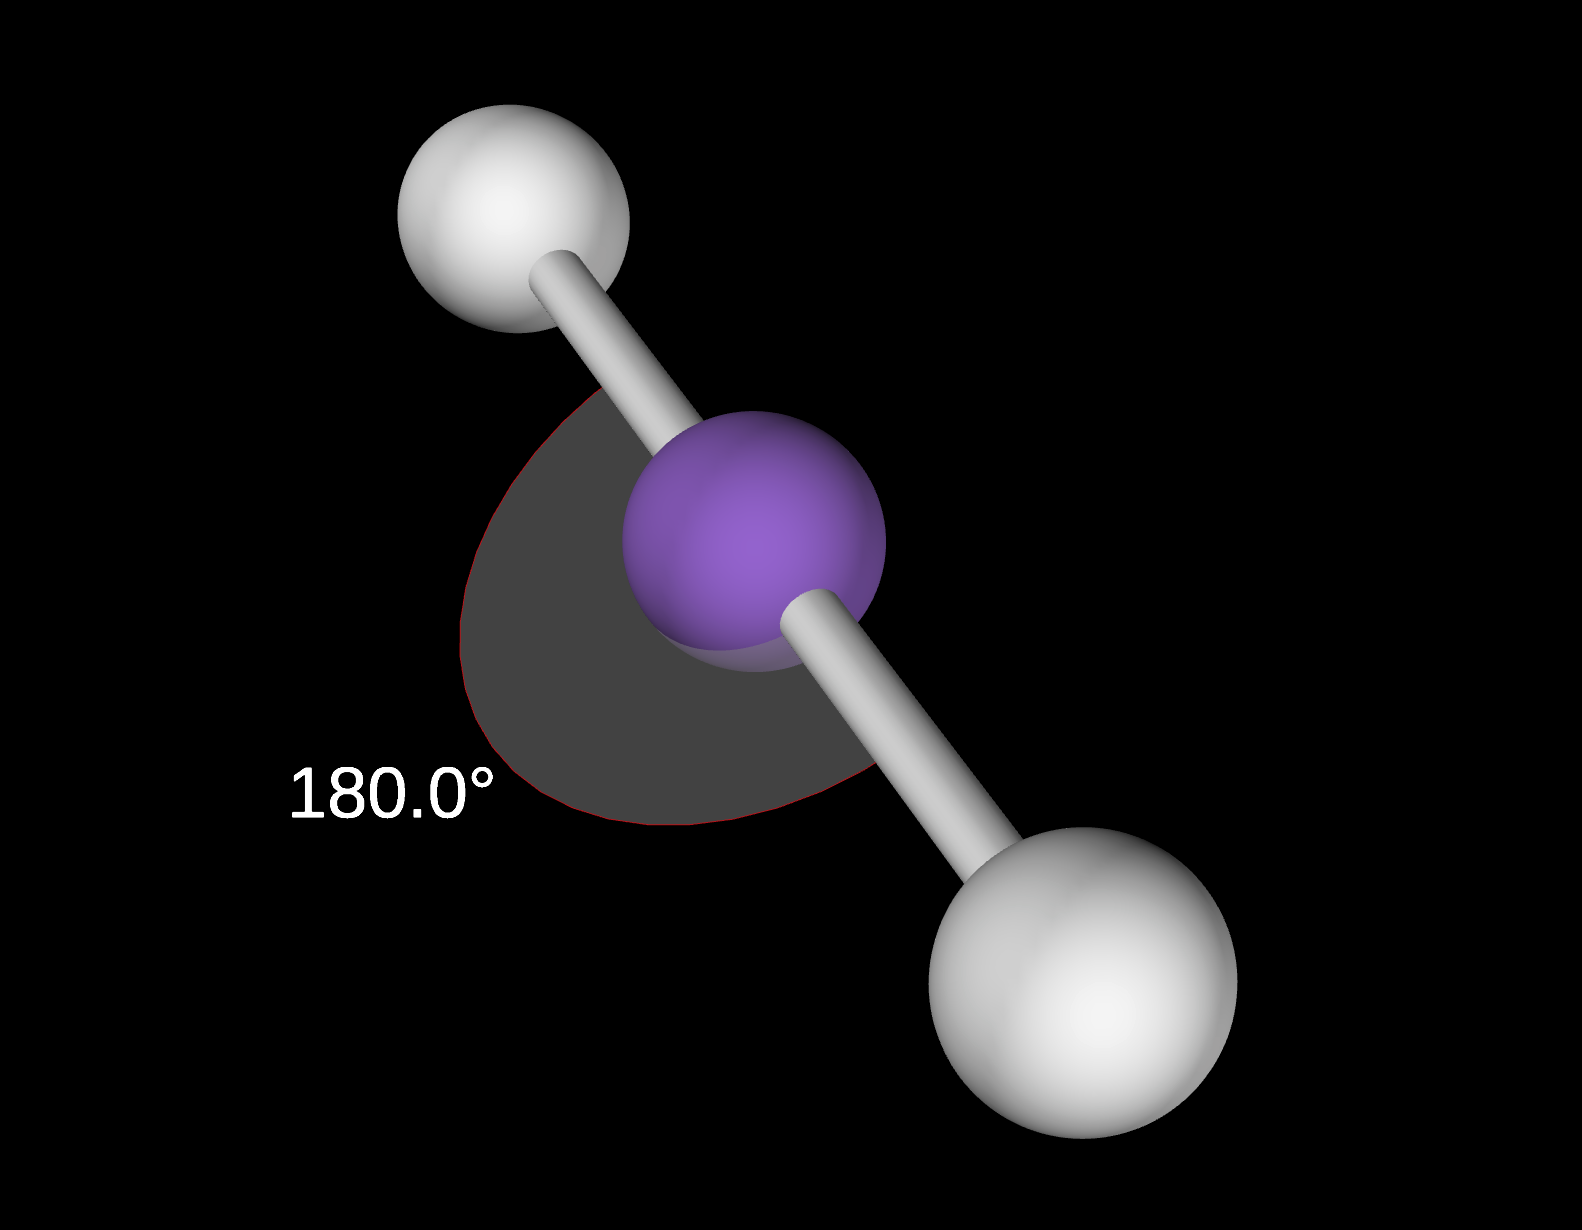
\includegraphics[width=\textwidth]{Screenshot 2026-06-05 at 10.13.02 PM.png}
        \caption{Linear geometry with a linear electron domain geometry.}
    \end{subfigure}
    \begin{subfigure}[t]{0.3\textwidth}
        \centering
        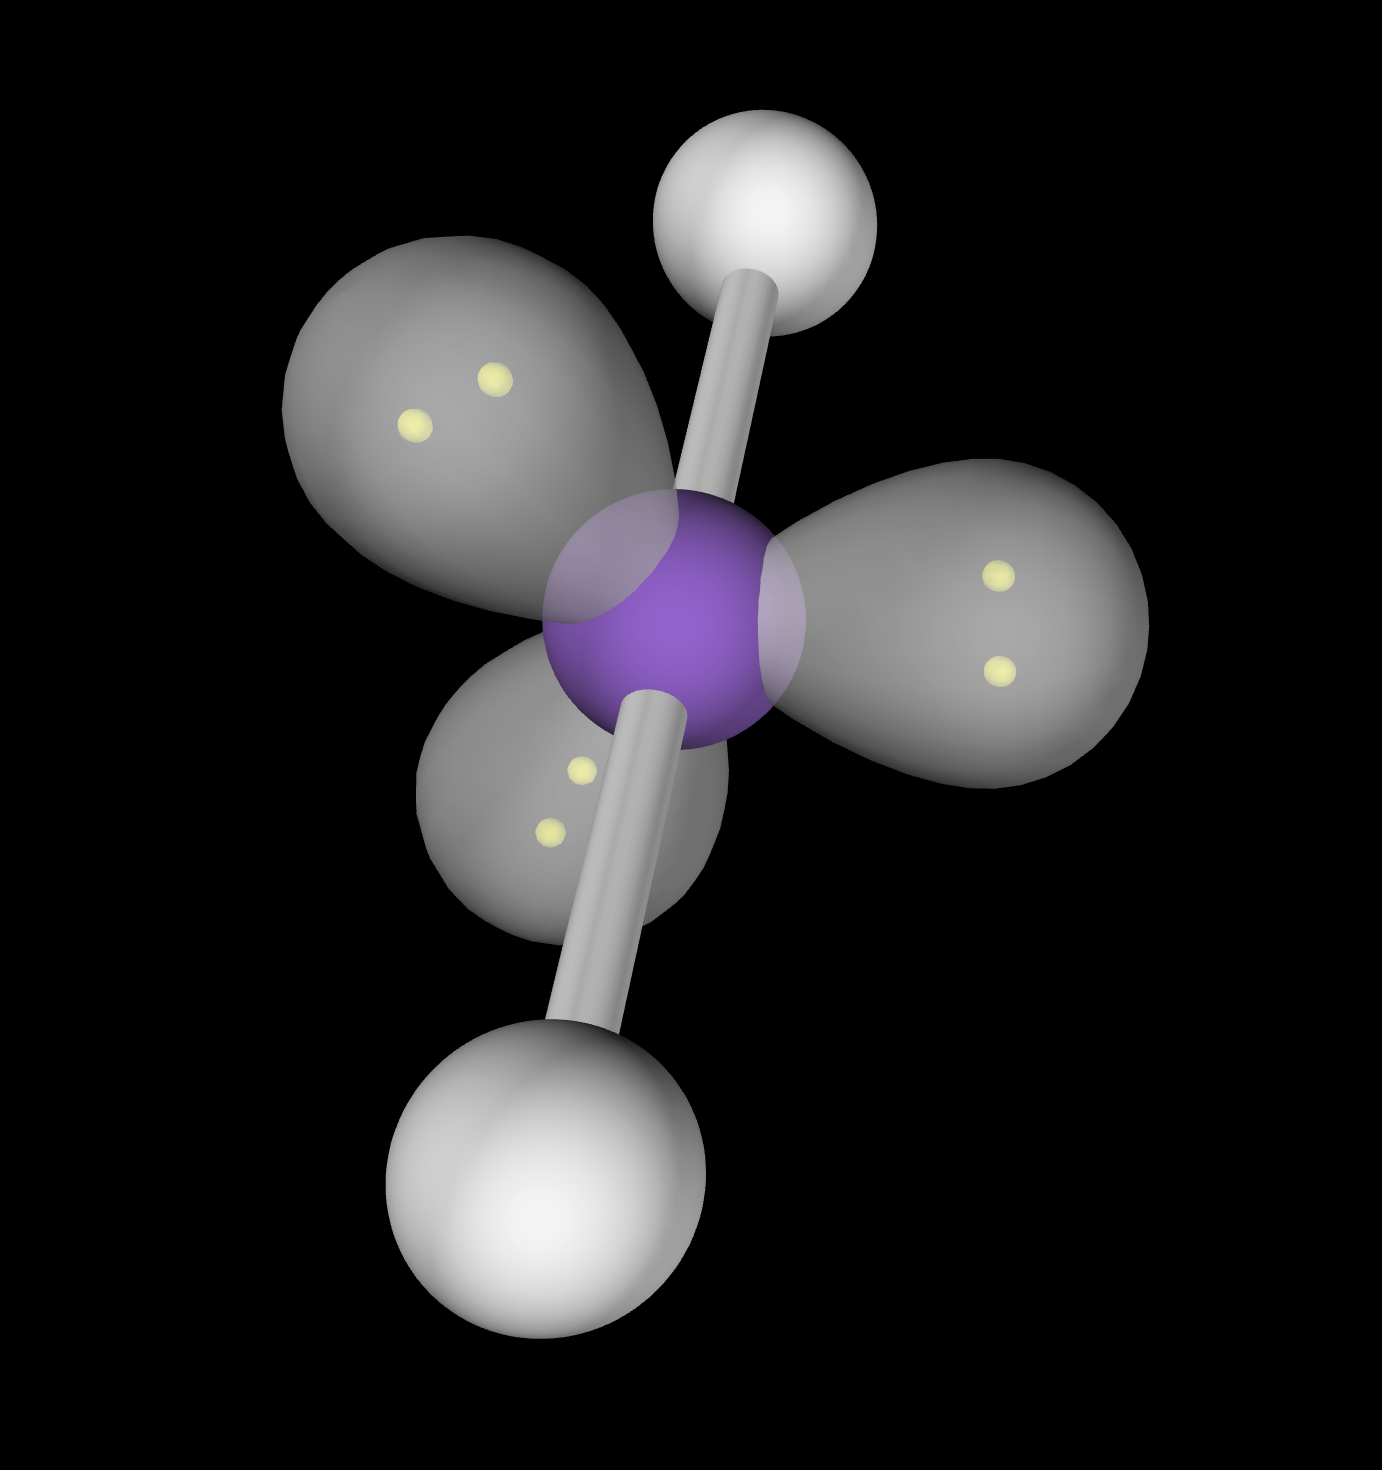
\includegraphics[width=\textwidth]{Screenshot 2026-06-05 at 10.13.30 PM.png}
        \caption{Linear geometry with a trigonal bipyramidal electron domain geometry.}
    \end{subfigure}
    \begin{subfigure}[t]{0.3\textwidth}
        \centering
        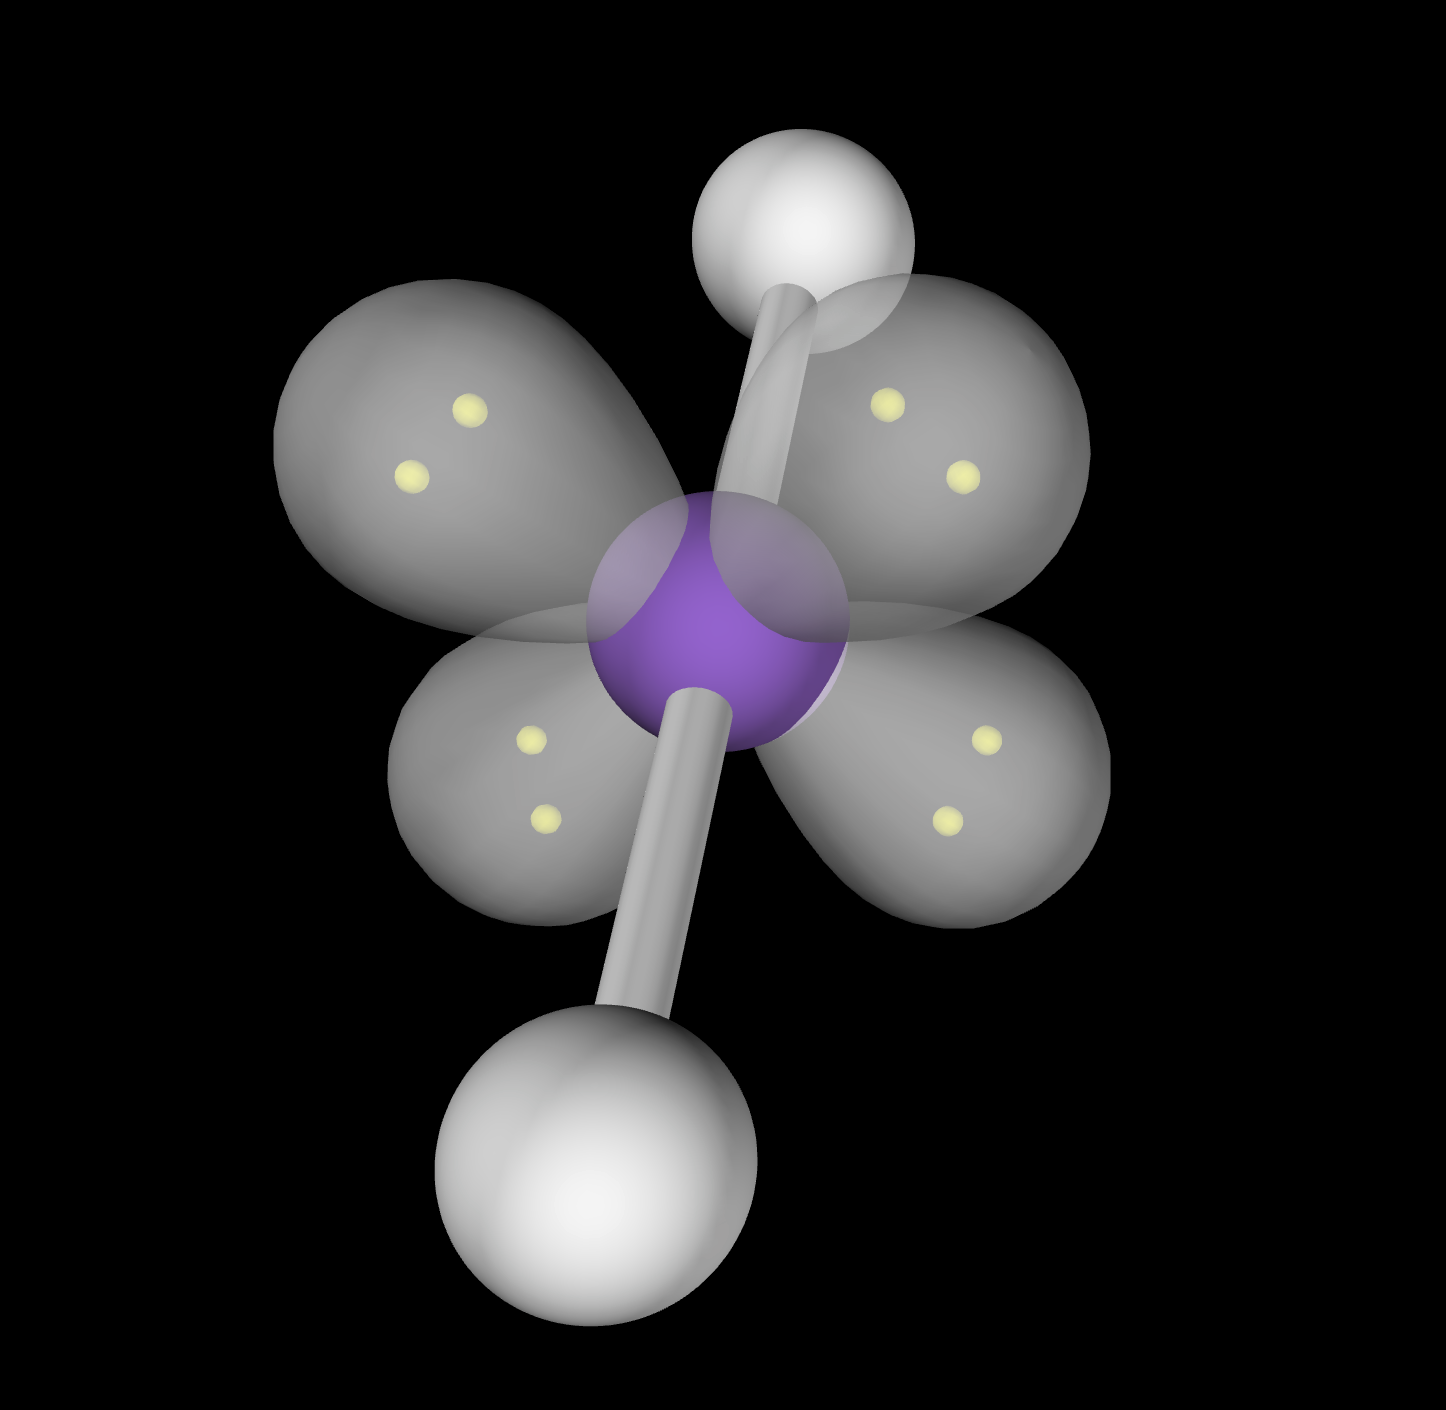
\includegraphics[width=\textwidth]{Screenshot 2026-06-05 at 10.13.34 PM.png}
        \caption{Linear geometry with an octahedral electron domain geometry.}
    \end{subfigure}
    \caption{Examples of linear molecular geometries.}
\end{figure*}
\subsubsection{Trigonal Planar Molecular Geometry}
The trigonal planar molecular geometry occurs when there are three electron pairs around the central atom, and all of them are bonding pairs. The bond angle in a trigonal planar molecule is 120\textdegree .
\begin{figure}[h]
    \centering
    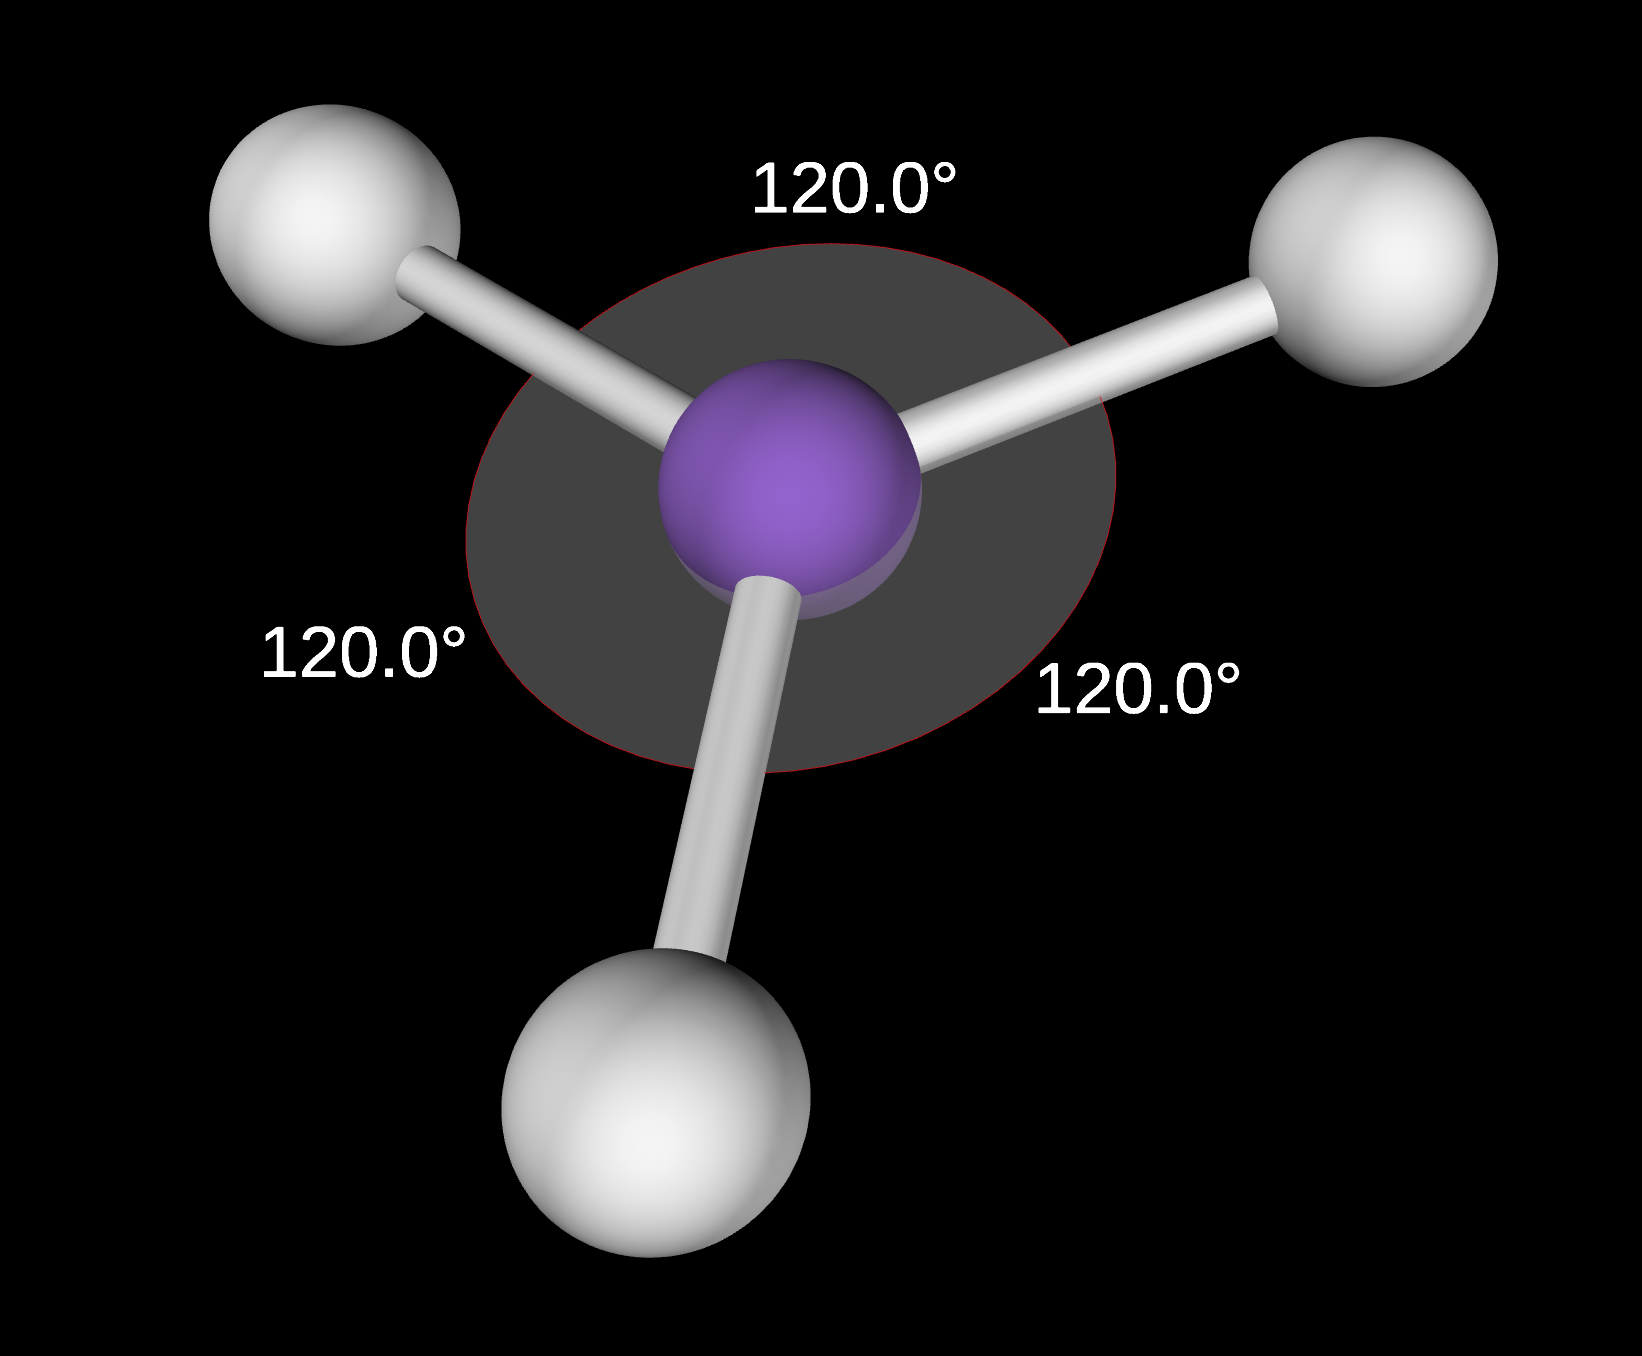
\includegraphics[width=0.4\textwidth]{Screenshot 2026-06-05 at 10.25.31 PM.png}
    \caption{Trigonal planar geometry with a trigonal planar electron domain geometry.}
\end{figure}
\subsubsection{Tetrahedral Molecular Geometry}
The tetrahedral molecular geometry occurs when there are four electron pairs around the central atom, and all of them are bonding pairs. The bond angle in a tetrahedral molecule is 109.5\textdegree .
\begin{figure}[h]
    \centering
    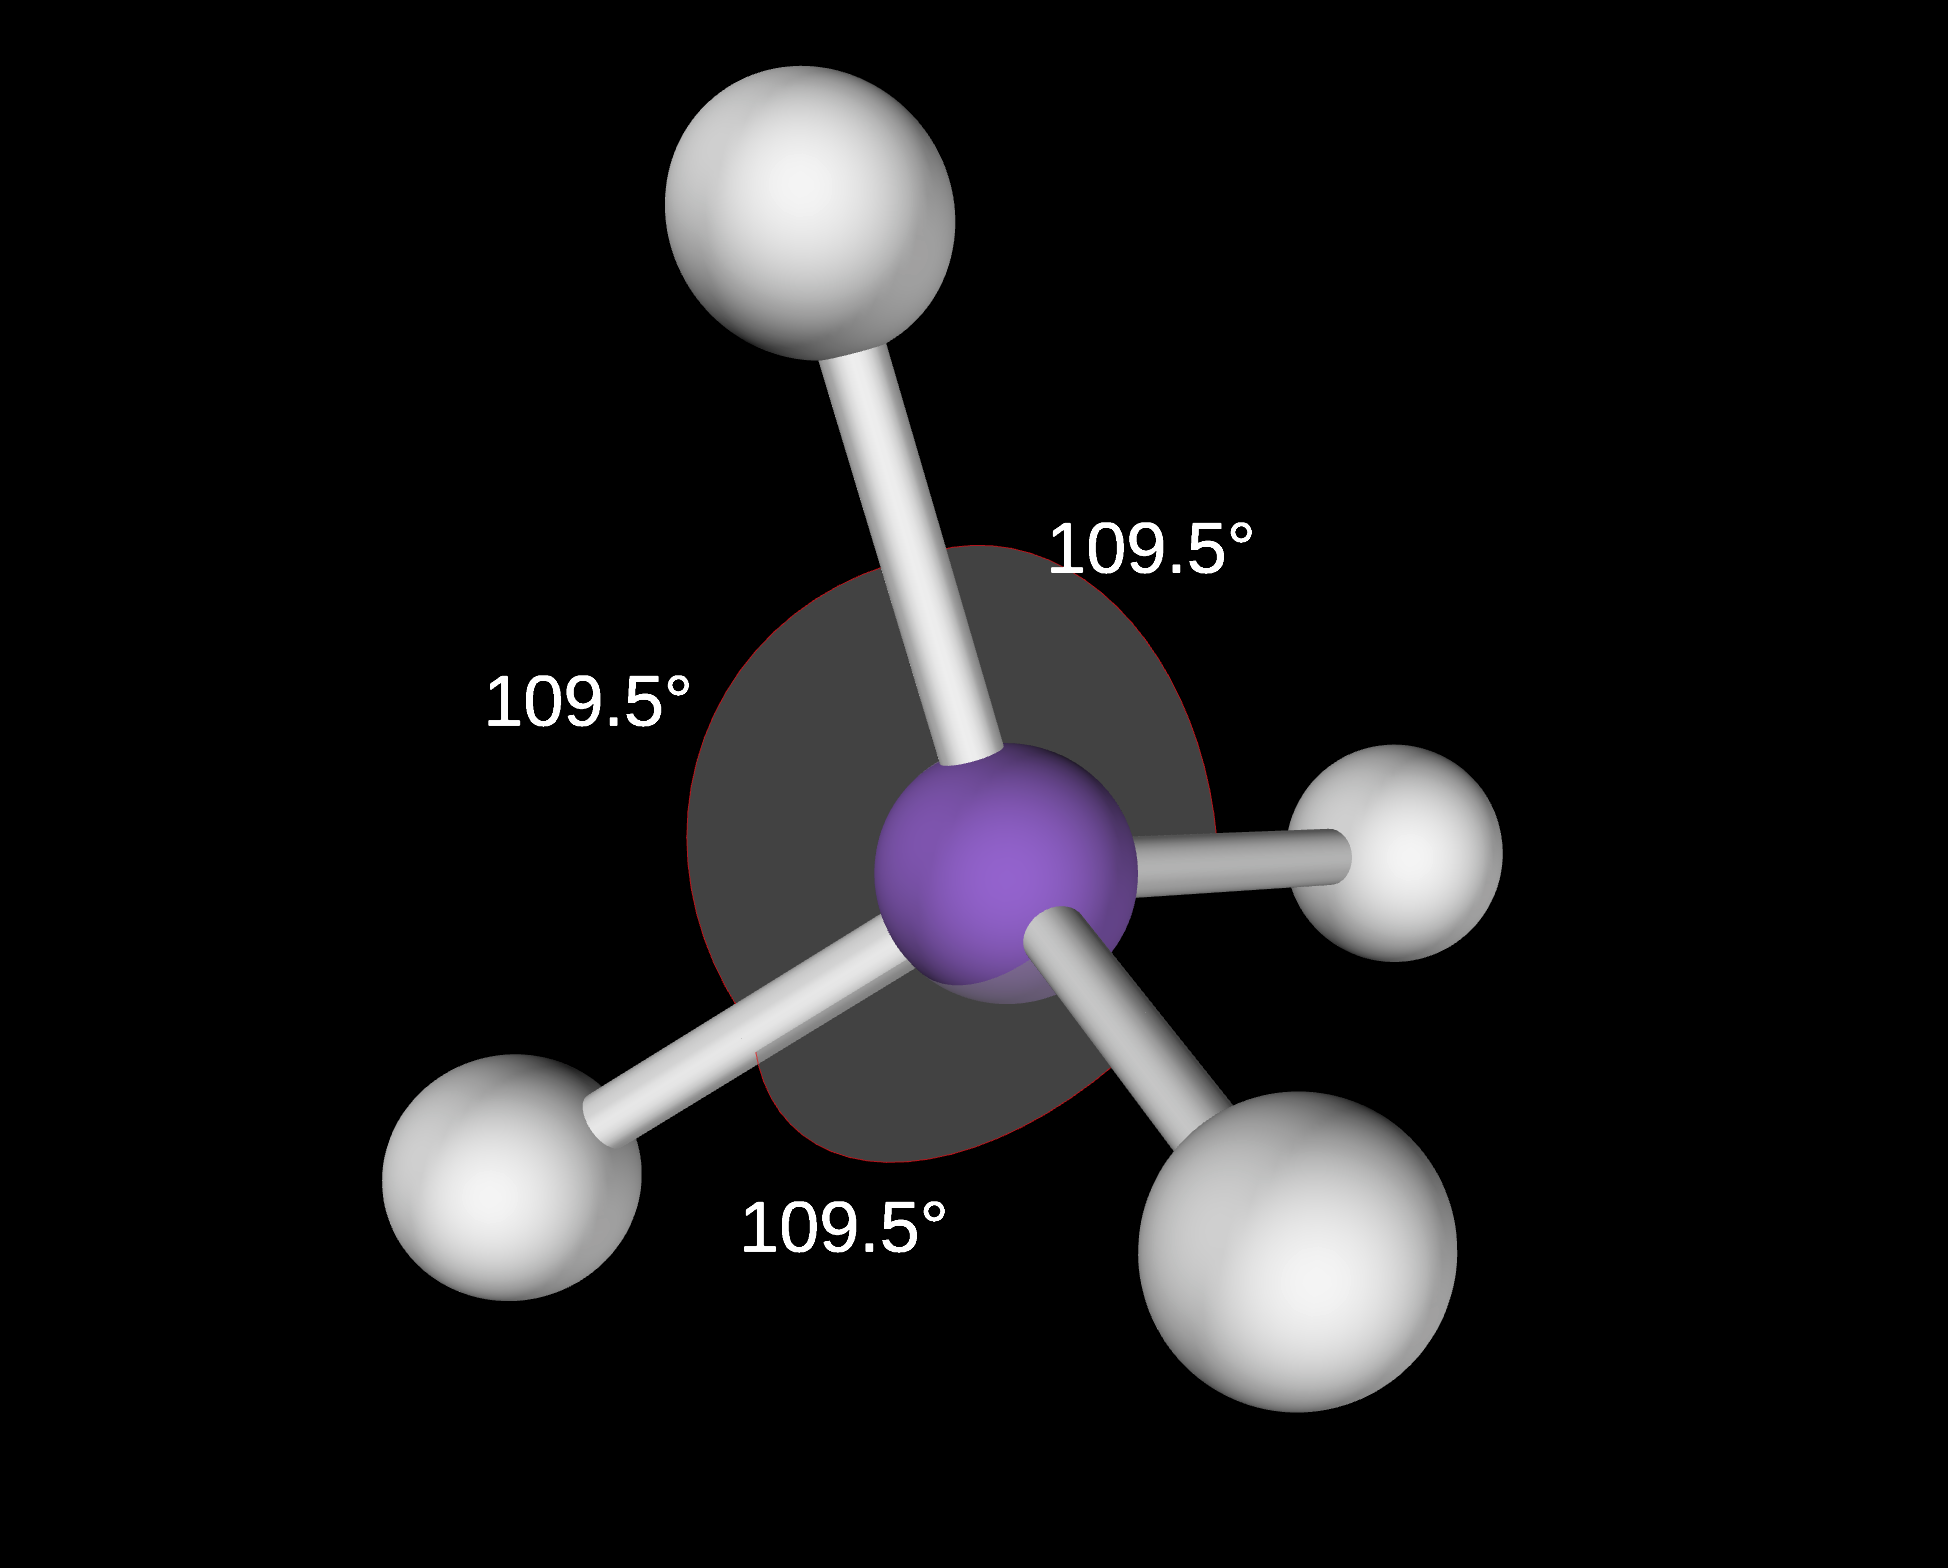
\includegraphics[width=0.4\textwidth]{Screenshot 2026-06-05 at 10.28.15 PM.png}
    \caption{Tetrahedral geometry with a tetrahedral electron domain geometry.}
\end{figure}
\subsubsection{Trigonal Pyramidal Molecular Geometry}
The trigonal pyramidal molecular geometry occurs when there are four electron pairs around the central atom, and three of them are bonding pairs while one of them is a lone pair. The bond angle in a trigonal pyramidal molecule is less than 109.5\textdegree  due to the repulsion from the lone pair pushing the bonding pairs closer together.
\begin{figure}[h]
    \centering
    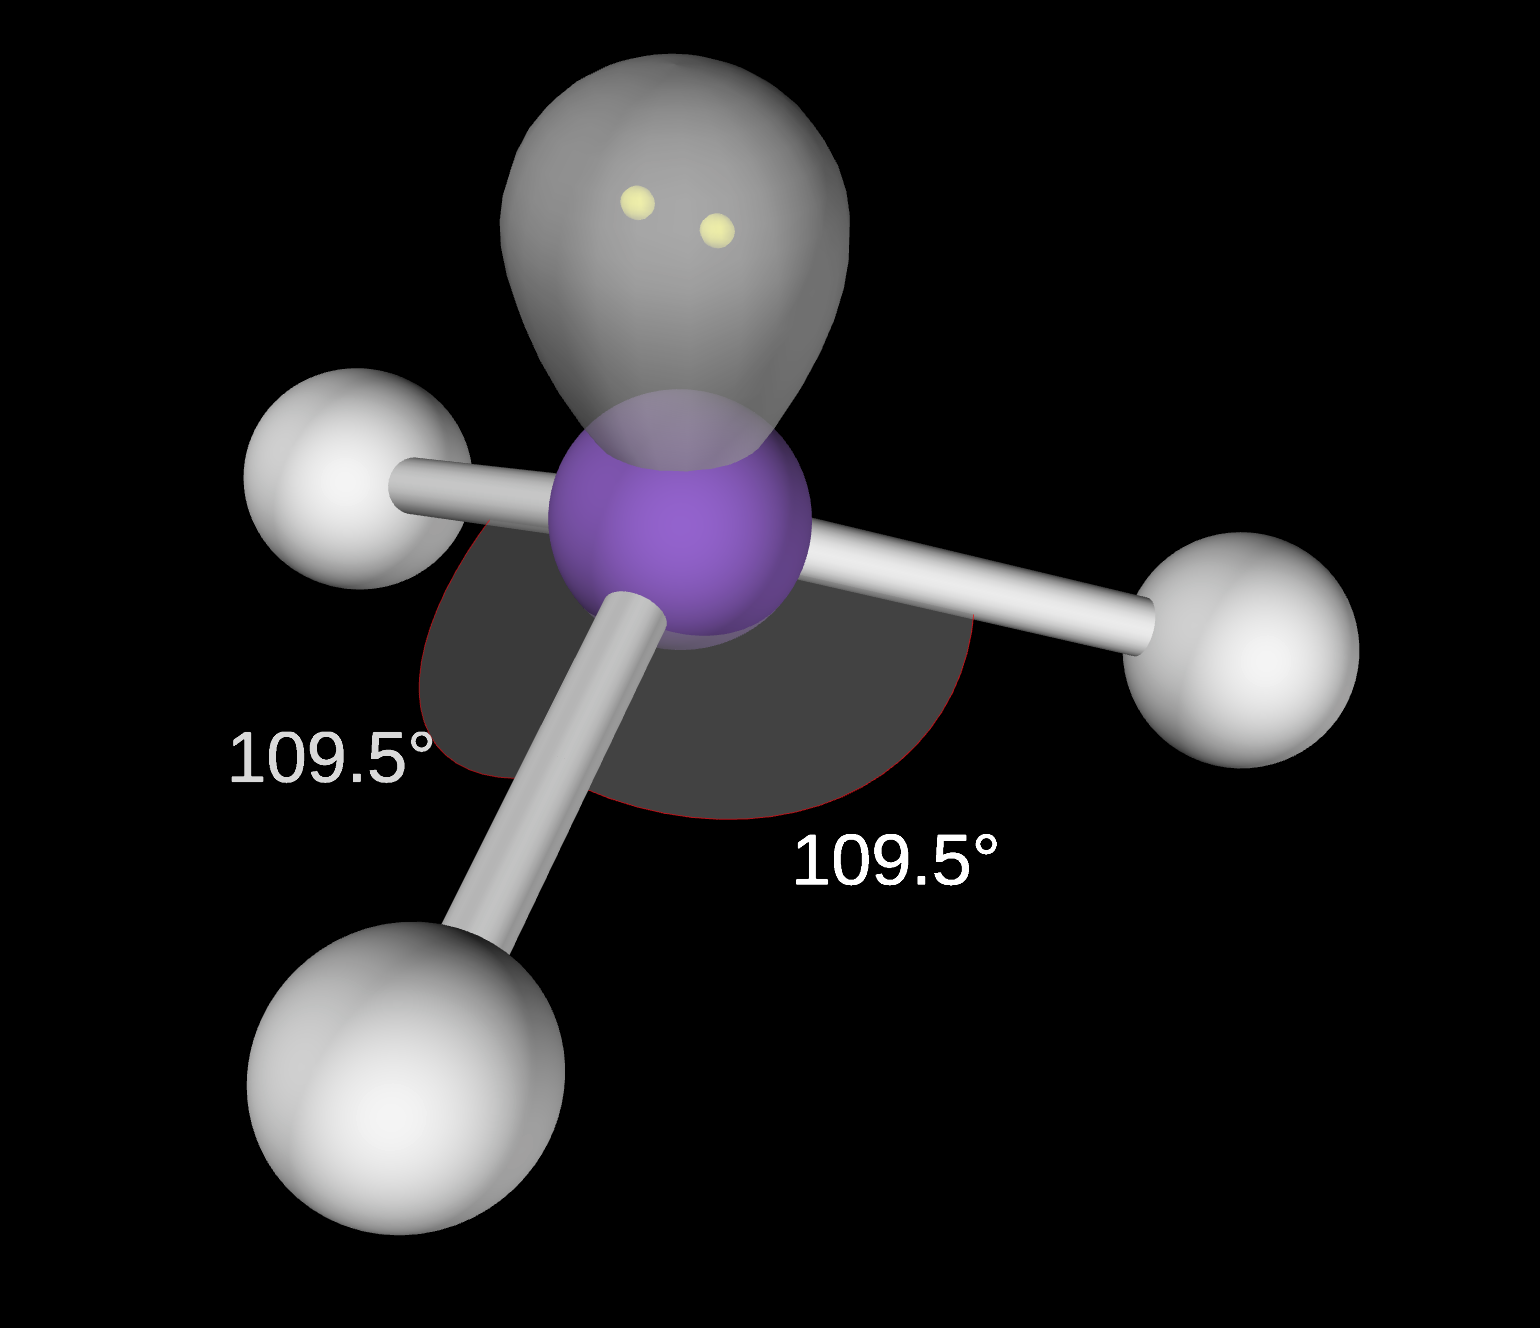
\includegraphics[width=0.4\textwidth]{Screenshot 2026-06-05 at 10.31.47 PM.png}
    \caption{Trigonal pyramidal geometry with a tetrahedral electron domain geometry.}
\end{figure}
\subsubsection{Bent Molecular Geometry}
The bent molecular geometry occurs when there are four electron pairs around the central atom, and two of them are bonding pairs while the other two are lone pairs. The bond angle in a bent molecule is less than 109.5\textdegree . The bent geometry can also occur when there are three electron pairs around the central atom, and two of them are bonding pairs while the other one is a lone pair. In this case, the bond angle is less than 120\textdegree . 
\begin{figure*}[h]
    \centering
    \begin{subfigure}[t]{0.4\textwidth}
        \centering
        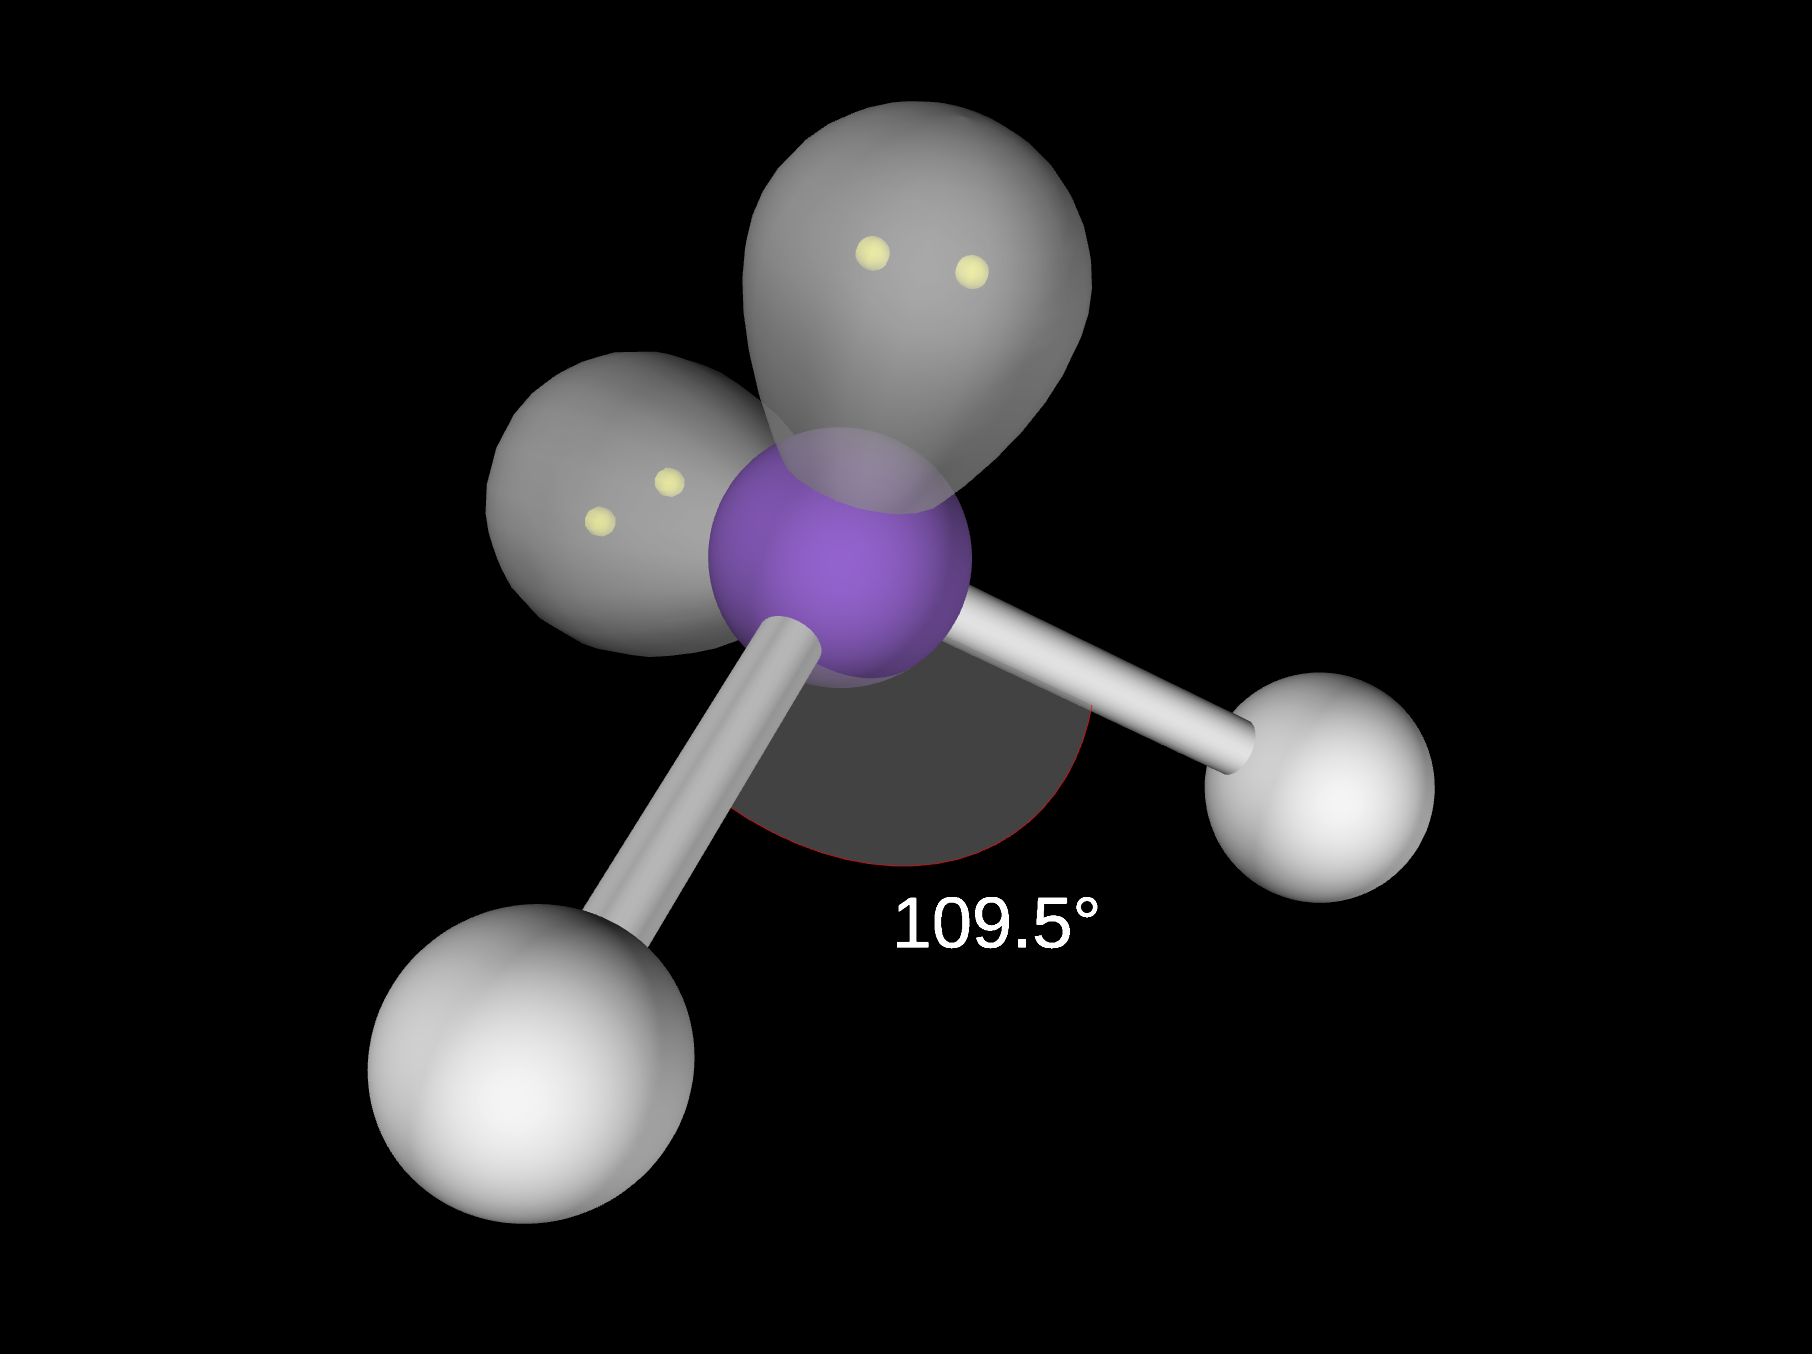
\includegraphics[width=\textwidth]{Screenshot 2026-06-05 at 10.33.31 PM.png}
        \caption{Bent geometry with a tetrahedral electron domain geometry.}
    \end{subfigure}
    \begin{subfigure}[t]{0.4\textwidth}
        \centering
        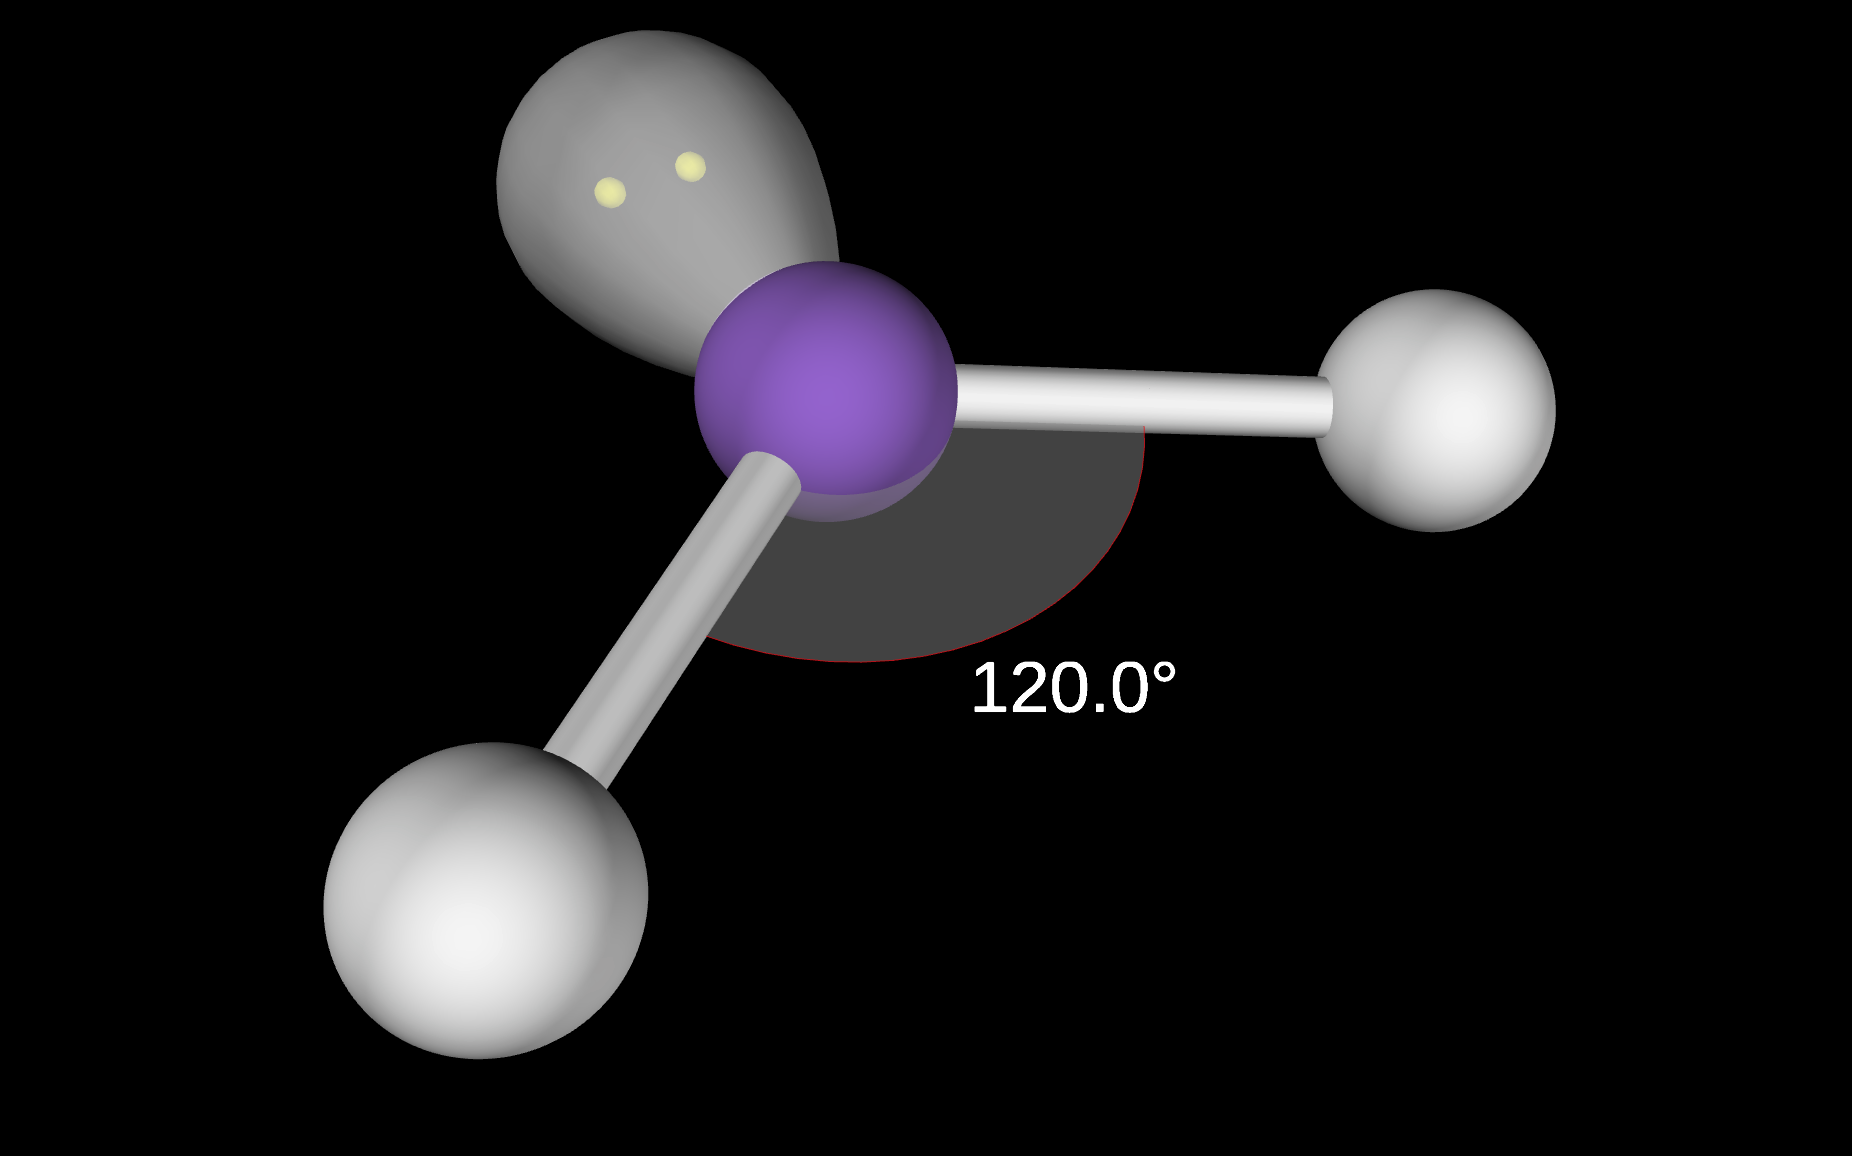
\includegraphics[width=\textwidth]{Screenshot 2026-06-05 at 10.34.14 PM.png}
        \caption{Bent geometry with a trigonal planar electron domain geometry.}
    \end{subfigure}
    \caption{Examples of bent molecular geometries.}
\end{figure*}
\subsubsection{See-Saw Molecular Geometry}
The see-saw molecular geometry occurs when there are five electron pairs around the central atom, and four of them are bonding pairs while one of them is a lone pair. The bond angles in a see-saw molecule are less than 120\textdegree  for the equatorial bonds and less than 90\textdegree  for the axial bonds. 
\begin{figure}[h]
    \centering
    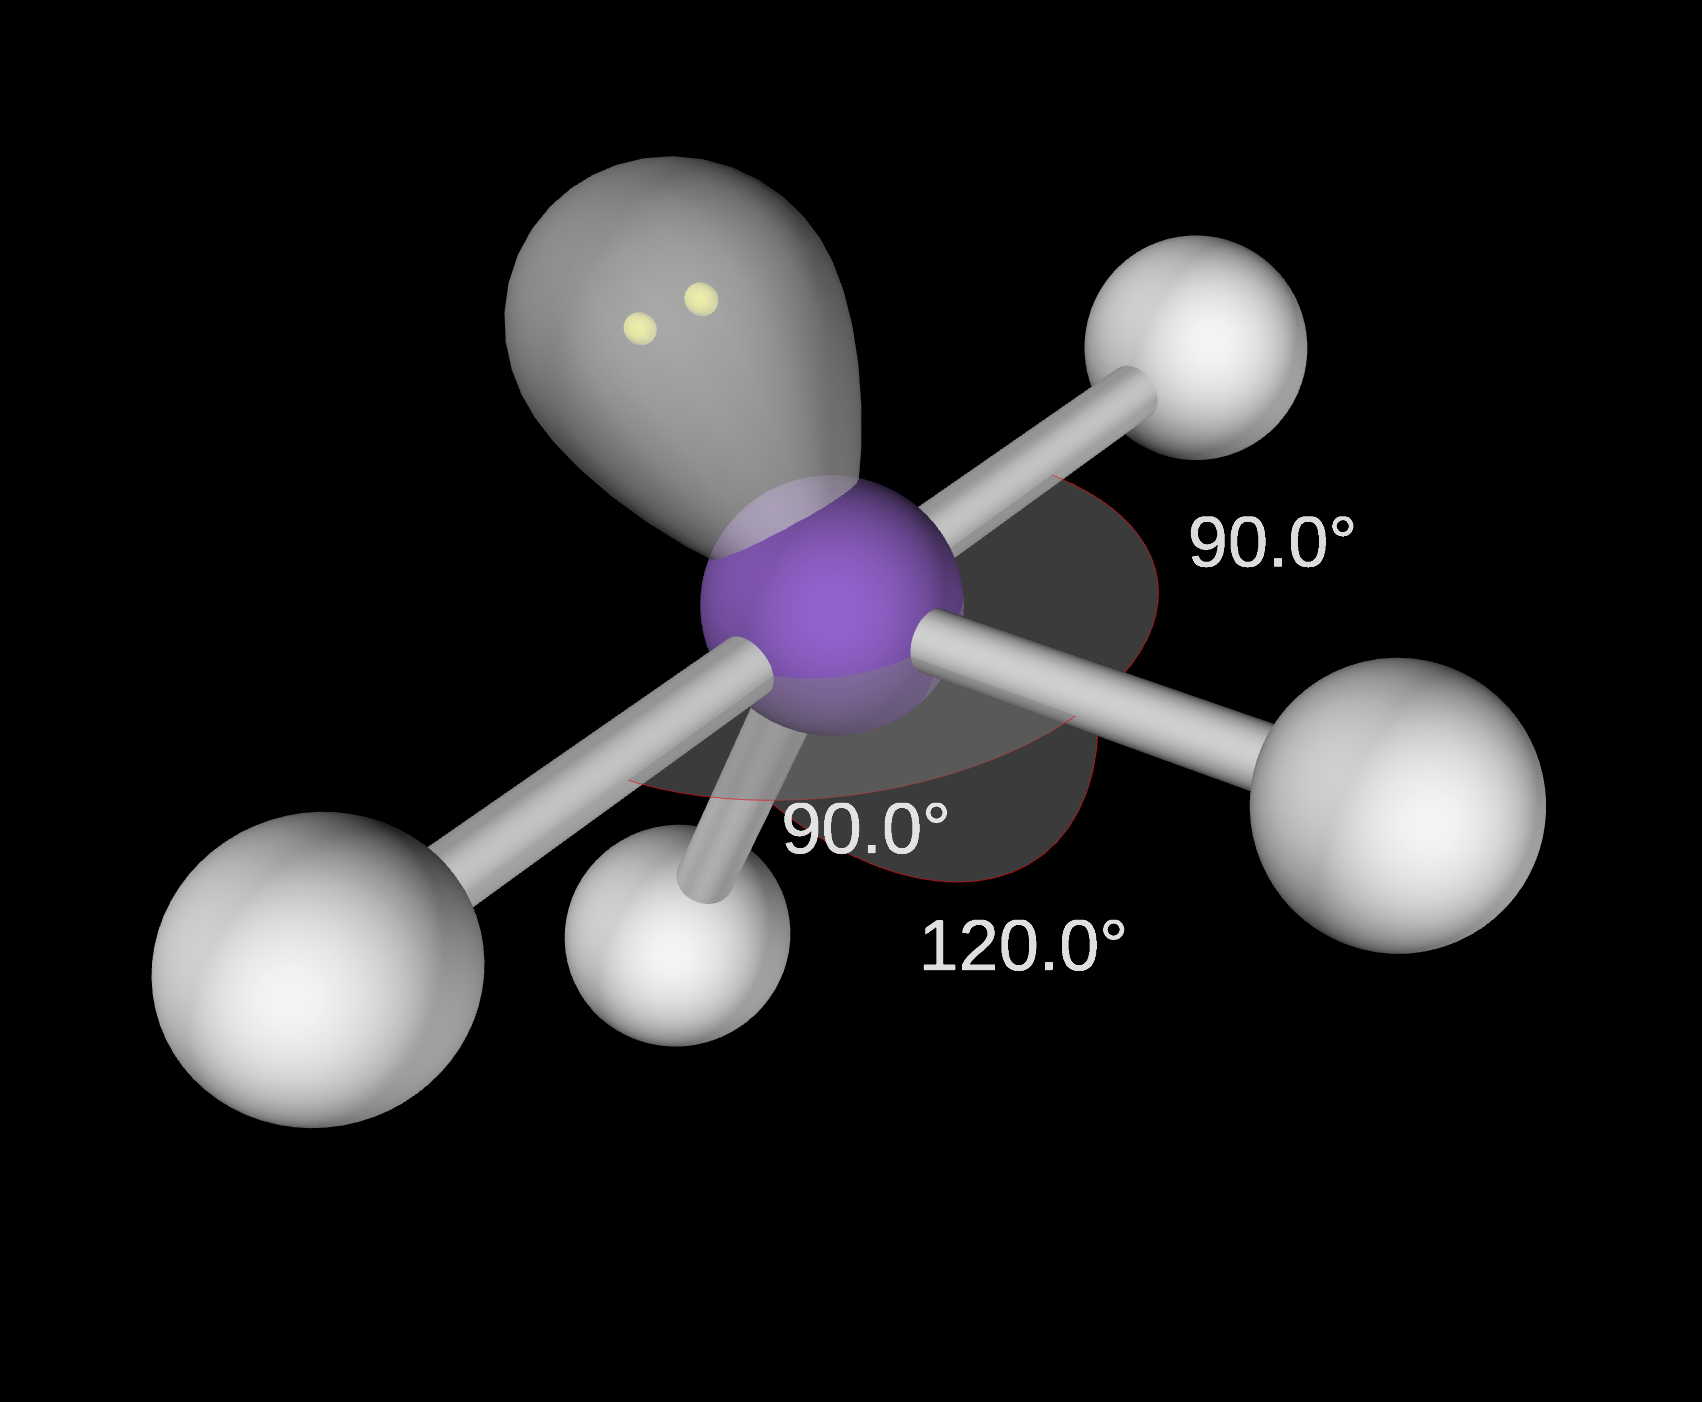
\includegraphics[width=0.4\textwidth]{Screenshot 2026-06-05 at 10.43.30 PM.png}
    \caption{See-saw geometry with a trigonal bipyramidal electron domain geometry.}
\end{figure}
\subsubsection{Trigonal Bipyramidal Molecular Geometry}
The trigonal bipyramidal molecular geometry occurs when there are five electron pairs around the central atom, and all of them are bonding pairs. The bond angles in a trigonal bipyramidal molecule are 120\textdegree  for the equatorial bonds and 90\textdegree  for the axial bonds. 
\begin{figure}[h]
    \centering
    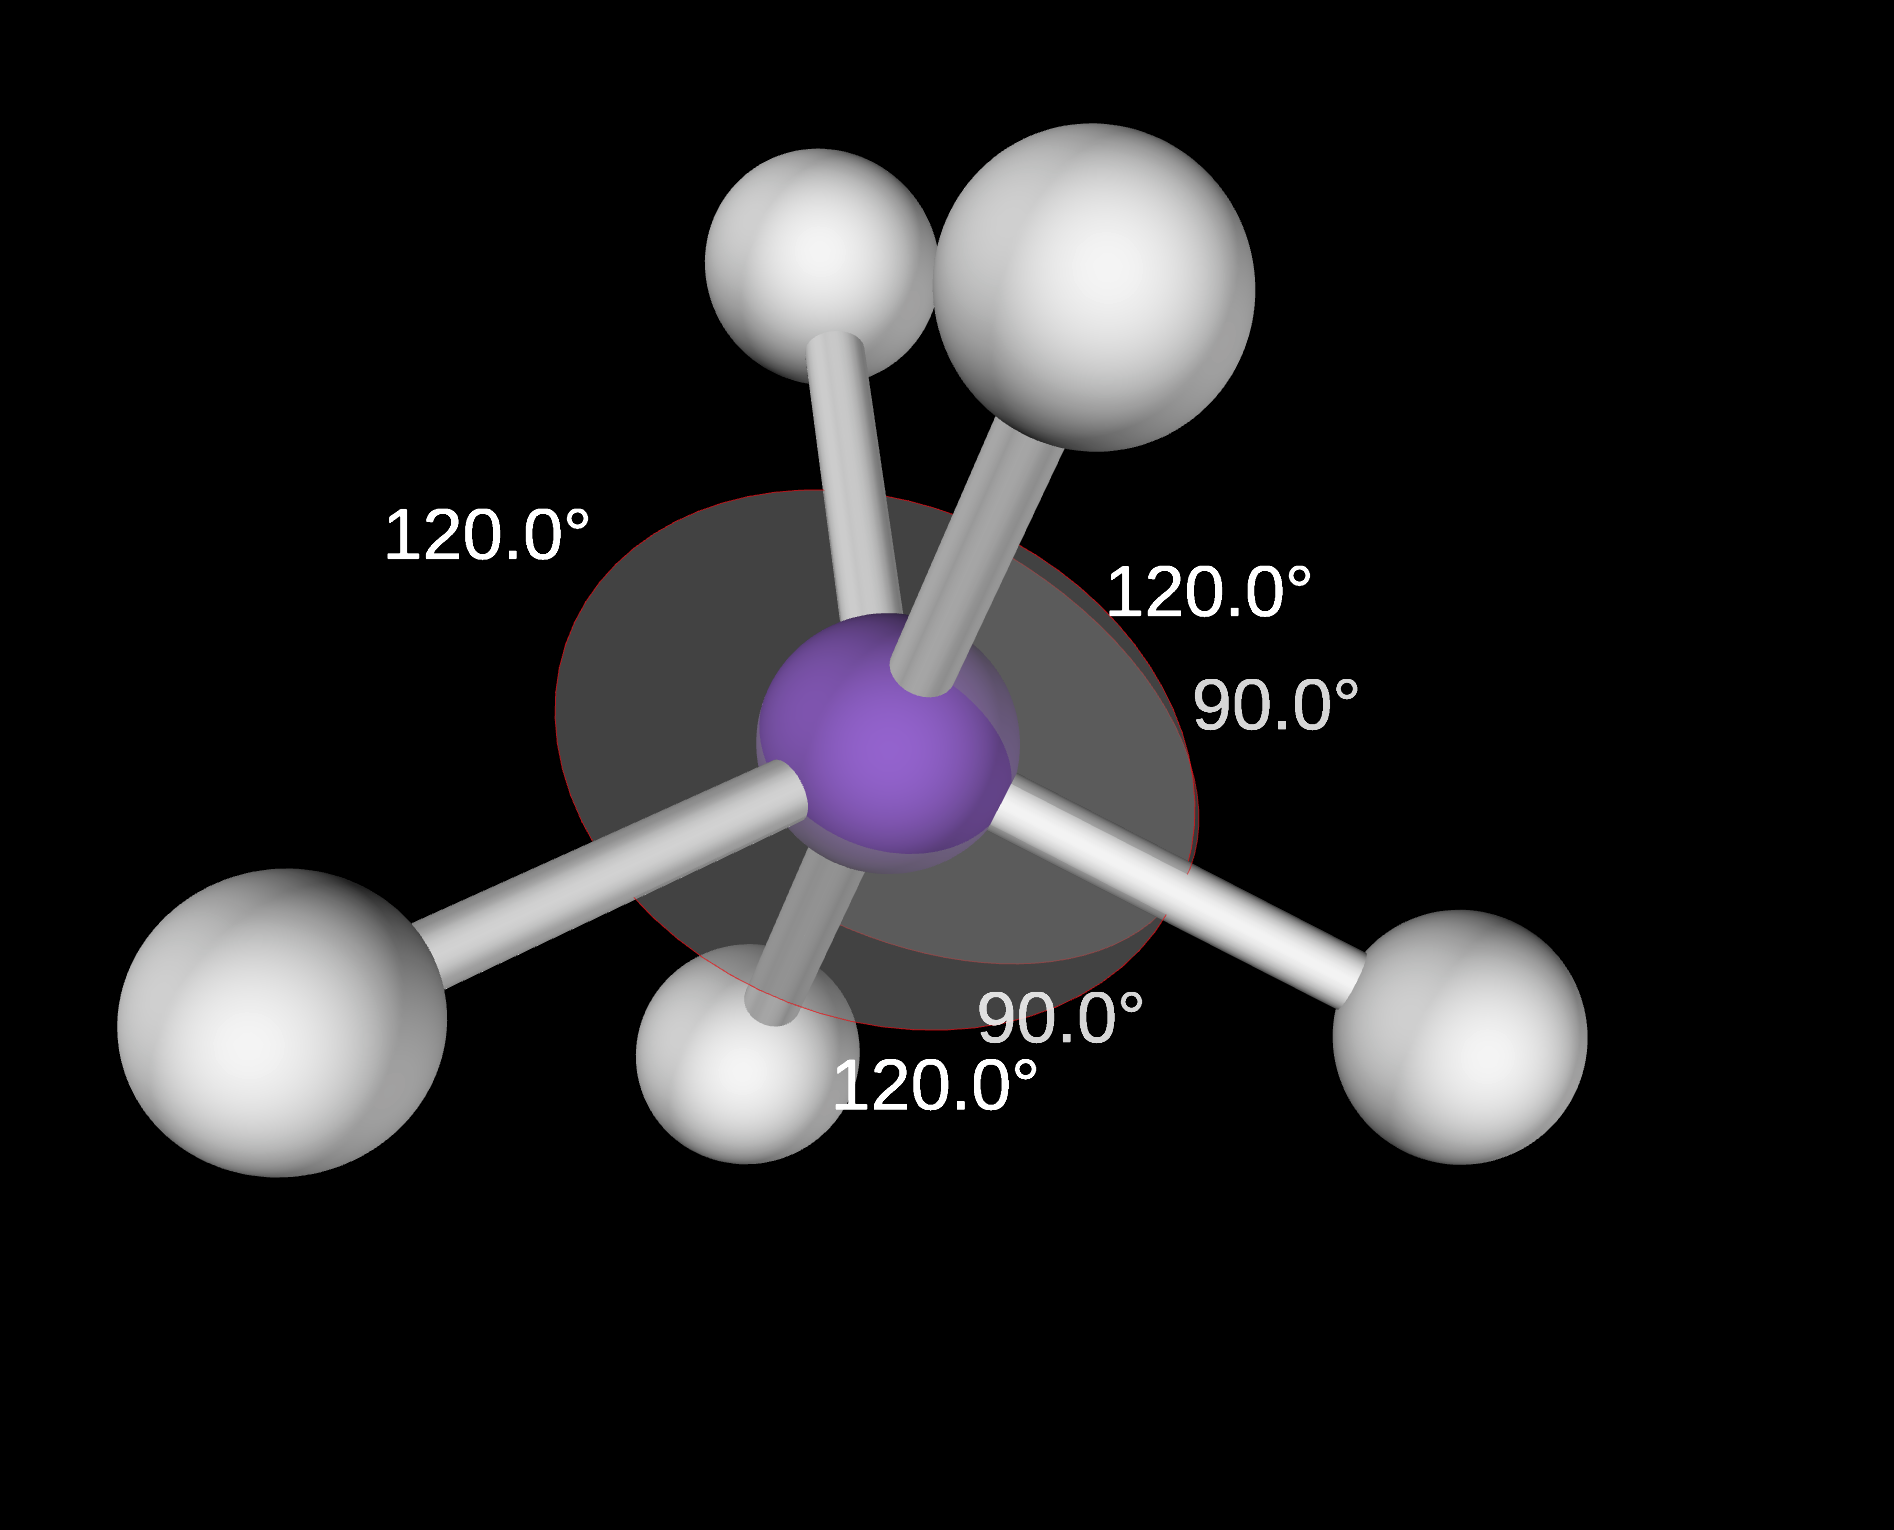
\includegraphics[width=0.4\textwidth]{Screenshot 2026-06-05 at 10.44.57 PM.png}
    \caption{Trigonal bipyramidal geometry with a trigonal bipyramidal electron domain geometry.}
\end{figure}
\subsubsection{T-Shaped Molecular Geometry}
The T-shaped molecular geometry occurs when there are five electron pairs around the central atom, and three of them are bonding pairs while the other two are lone pairs. The bond angles in a T-shaped molecule are less than 90\textdegree .
\begin{figure}[h]
    \centering
    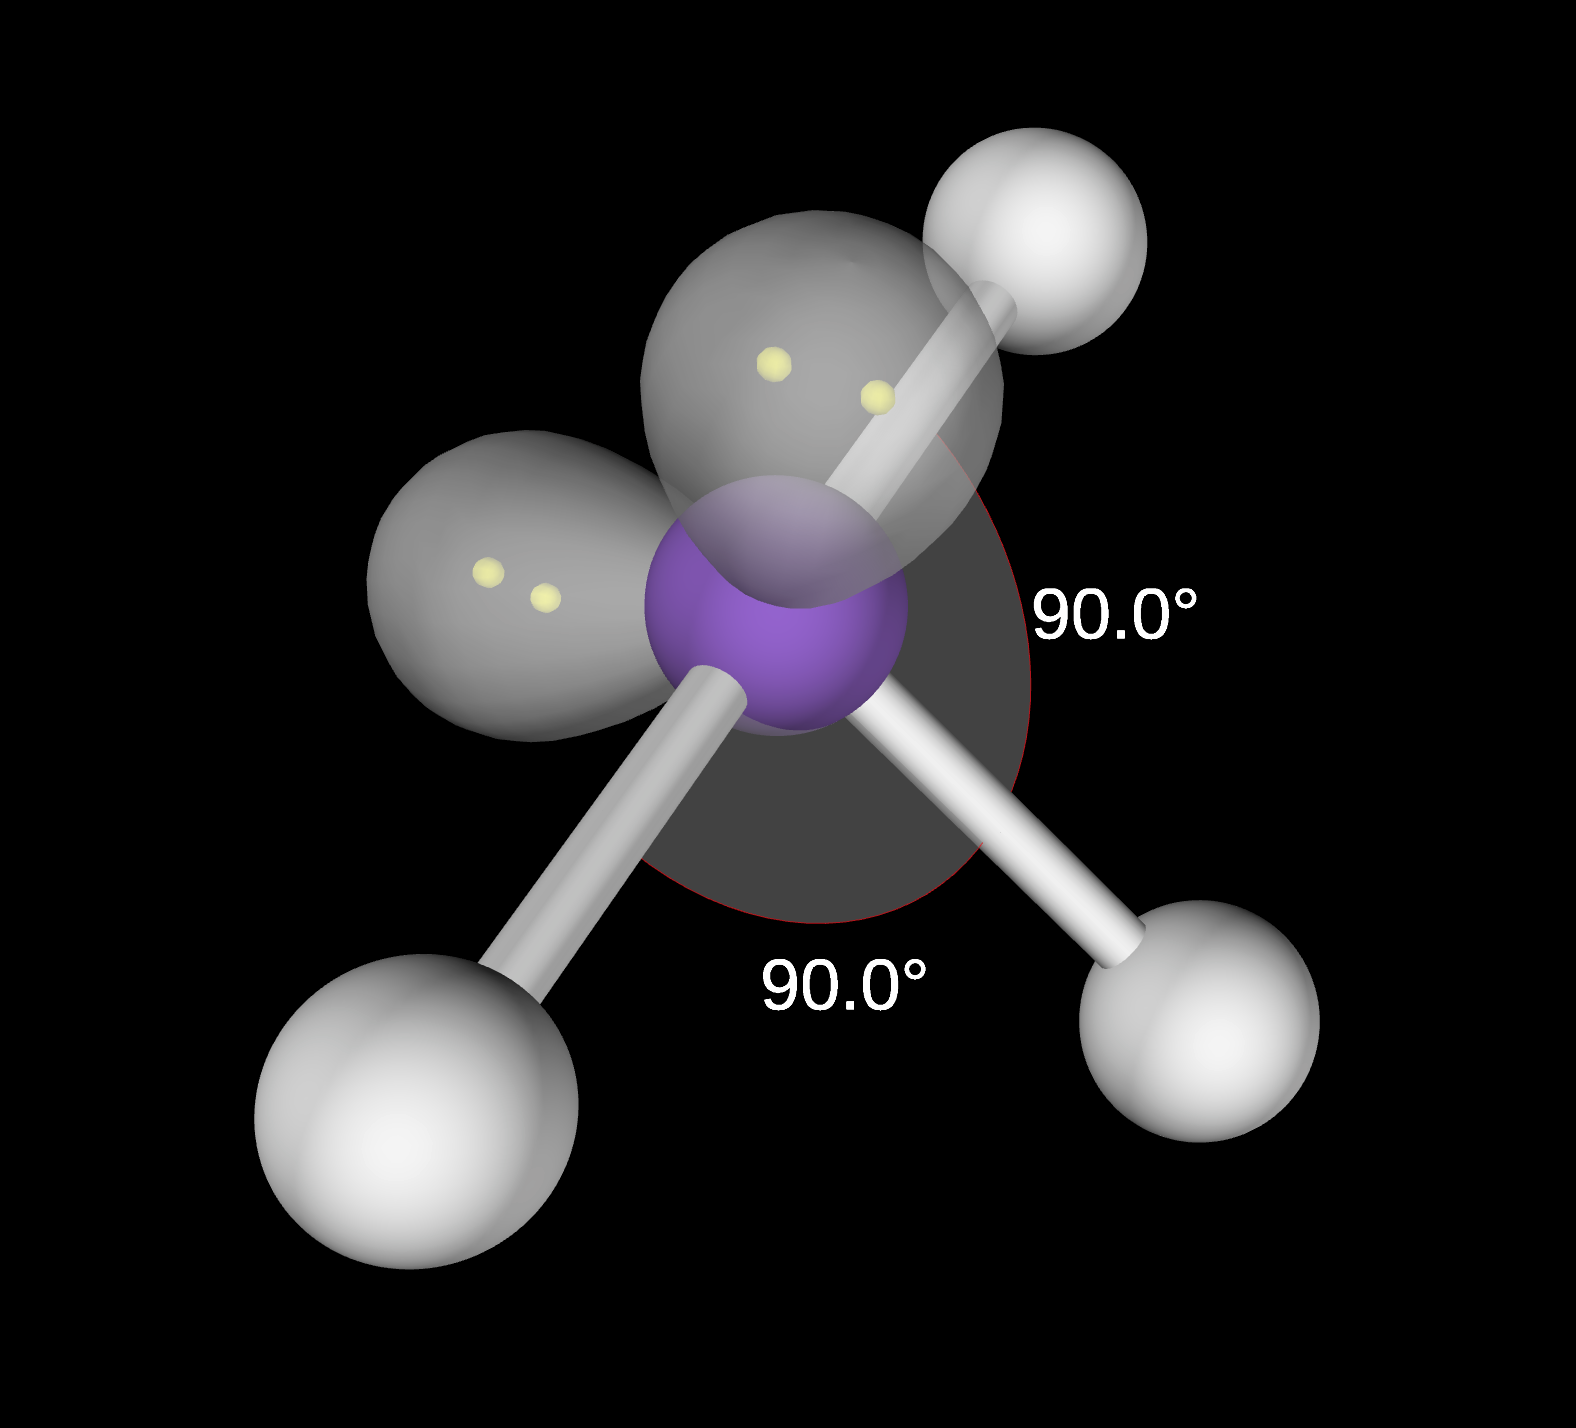
\includegraphics[width=0.4\textwidth]{Screenshot 2026-06-05 at 10.45.53 PM.png}
    \caption{T-shaped geometry with a trigonal bipyramidal electron domain geometry.}
\end{figure}
\subsubsection{Square Pyramidal Molecular Geometry}
The square pyramidal molecular geometry occurs when there are six electron pairs around the central atom, and five of them are bonding pairs while one of them is a lone pair. The bond angles in a square pyramidal molecule are less than 90\textdegree  for the bonds in the square base and less than 90\textdegree  for the bond between the central atom and the apex of the pyramid. 
\begin{figure}[h]
    \centering
    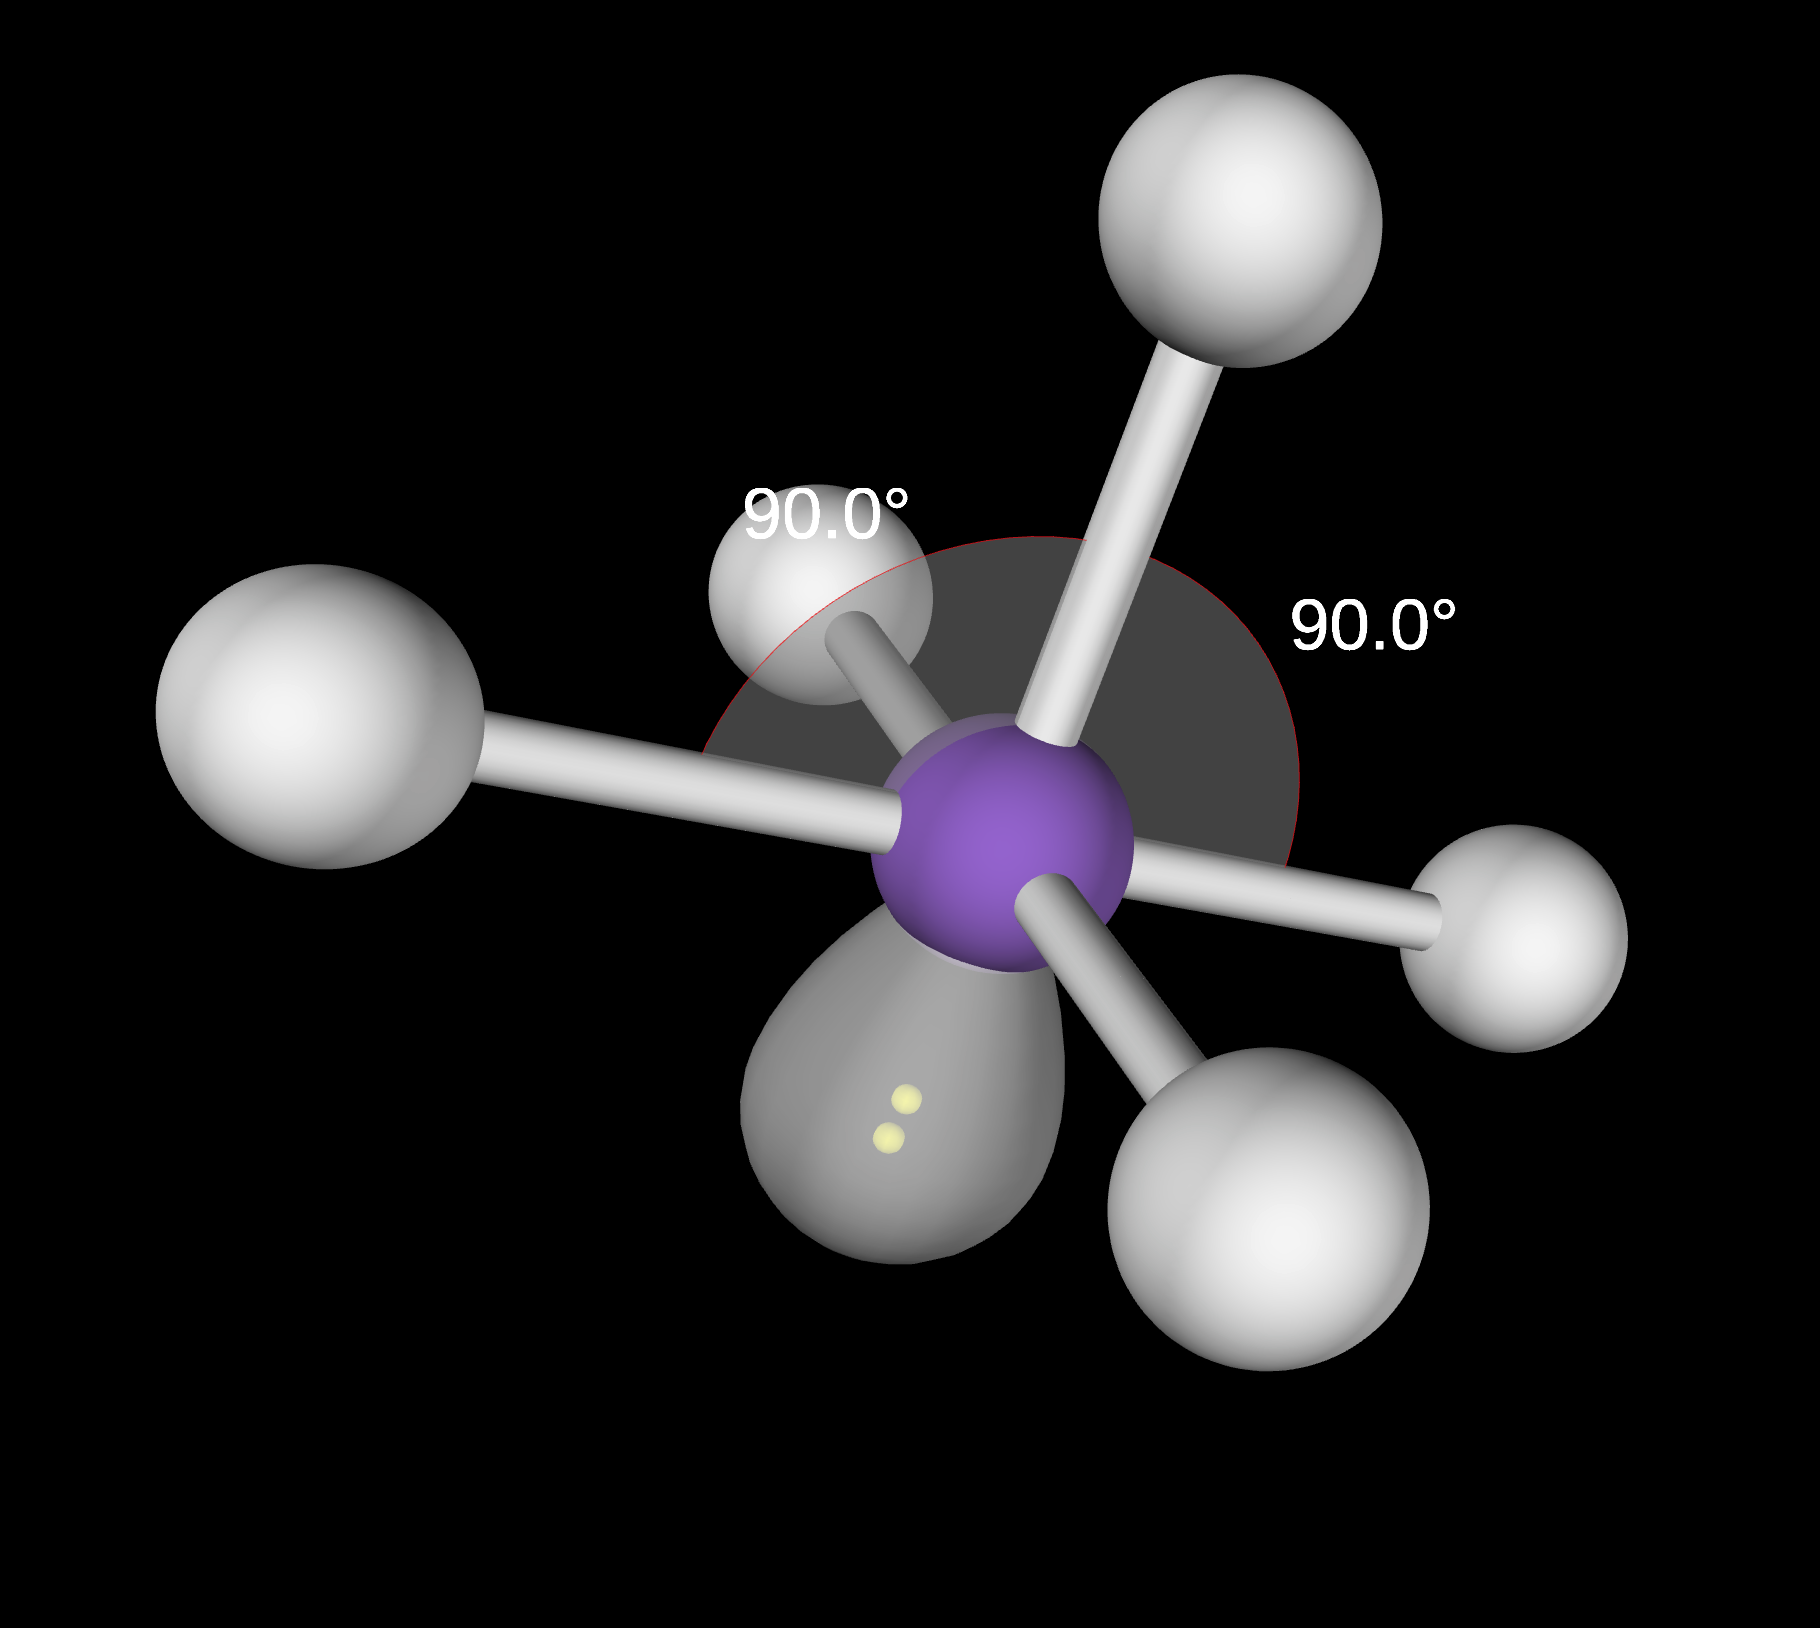
\includegraphics[width=0.4\textwidth]{Screenshot 2026-06-05 at 10.47.14 PM.png}
    \caption{Square pyramidal geometry with an octahedral electron domain geometry.}
\end{figure}
\subsubsection{Octahedral Molecular Geometry}
The octahedral molecular geometry occurs when there are six electron pairs around the central atom, and all of them are bonding pairs. The bond angles in an octahedral molecule are 90\textdegree  for all bonds. 
\begin{figure}[h]
    \centering
    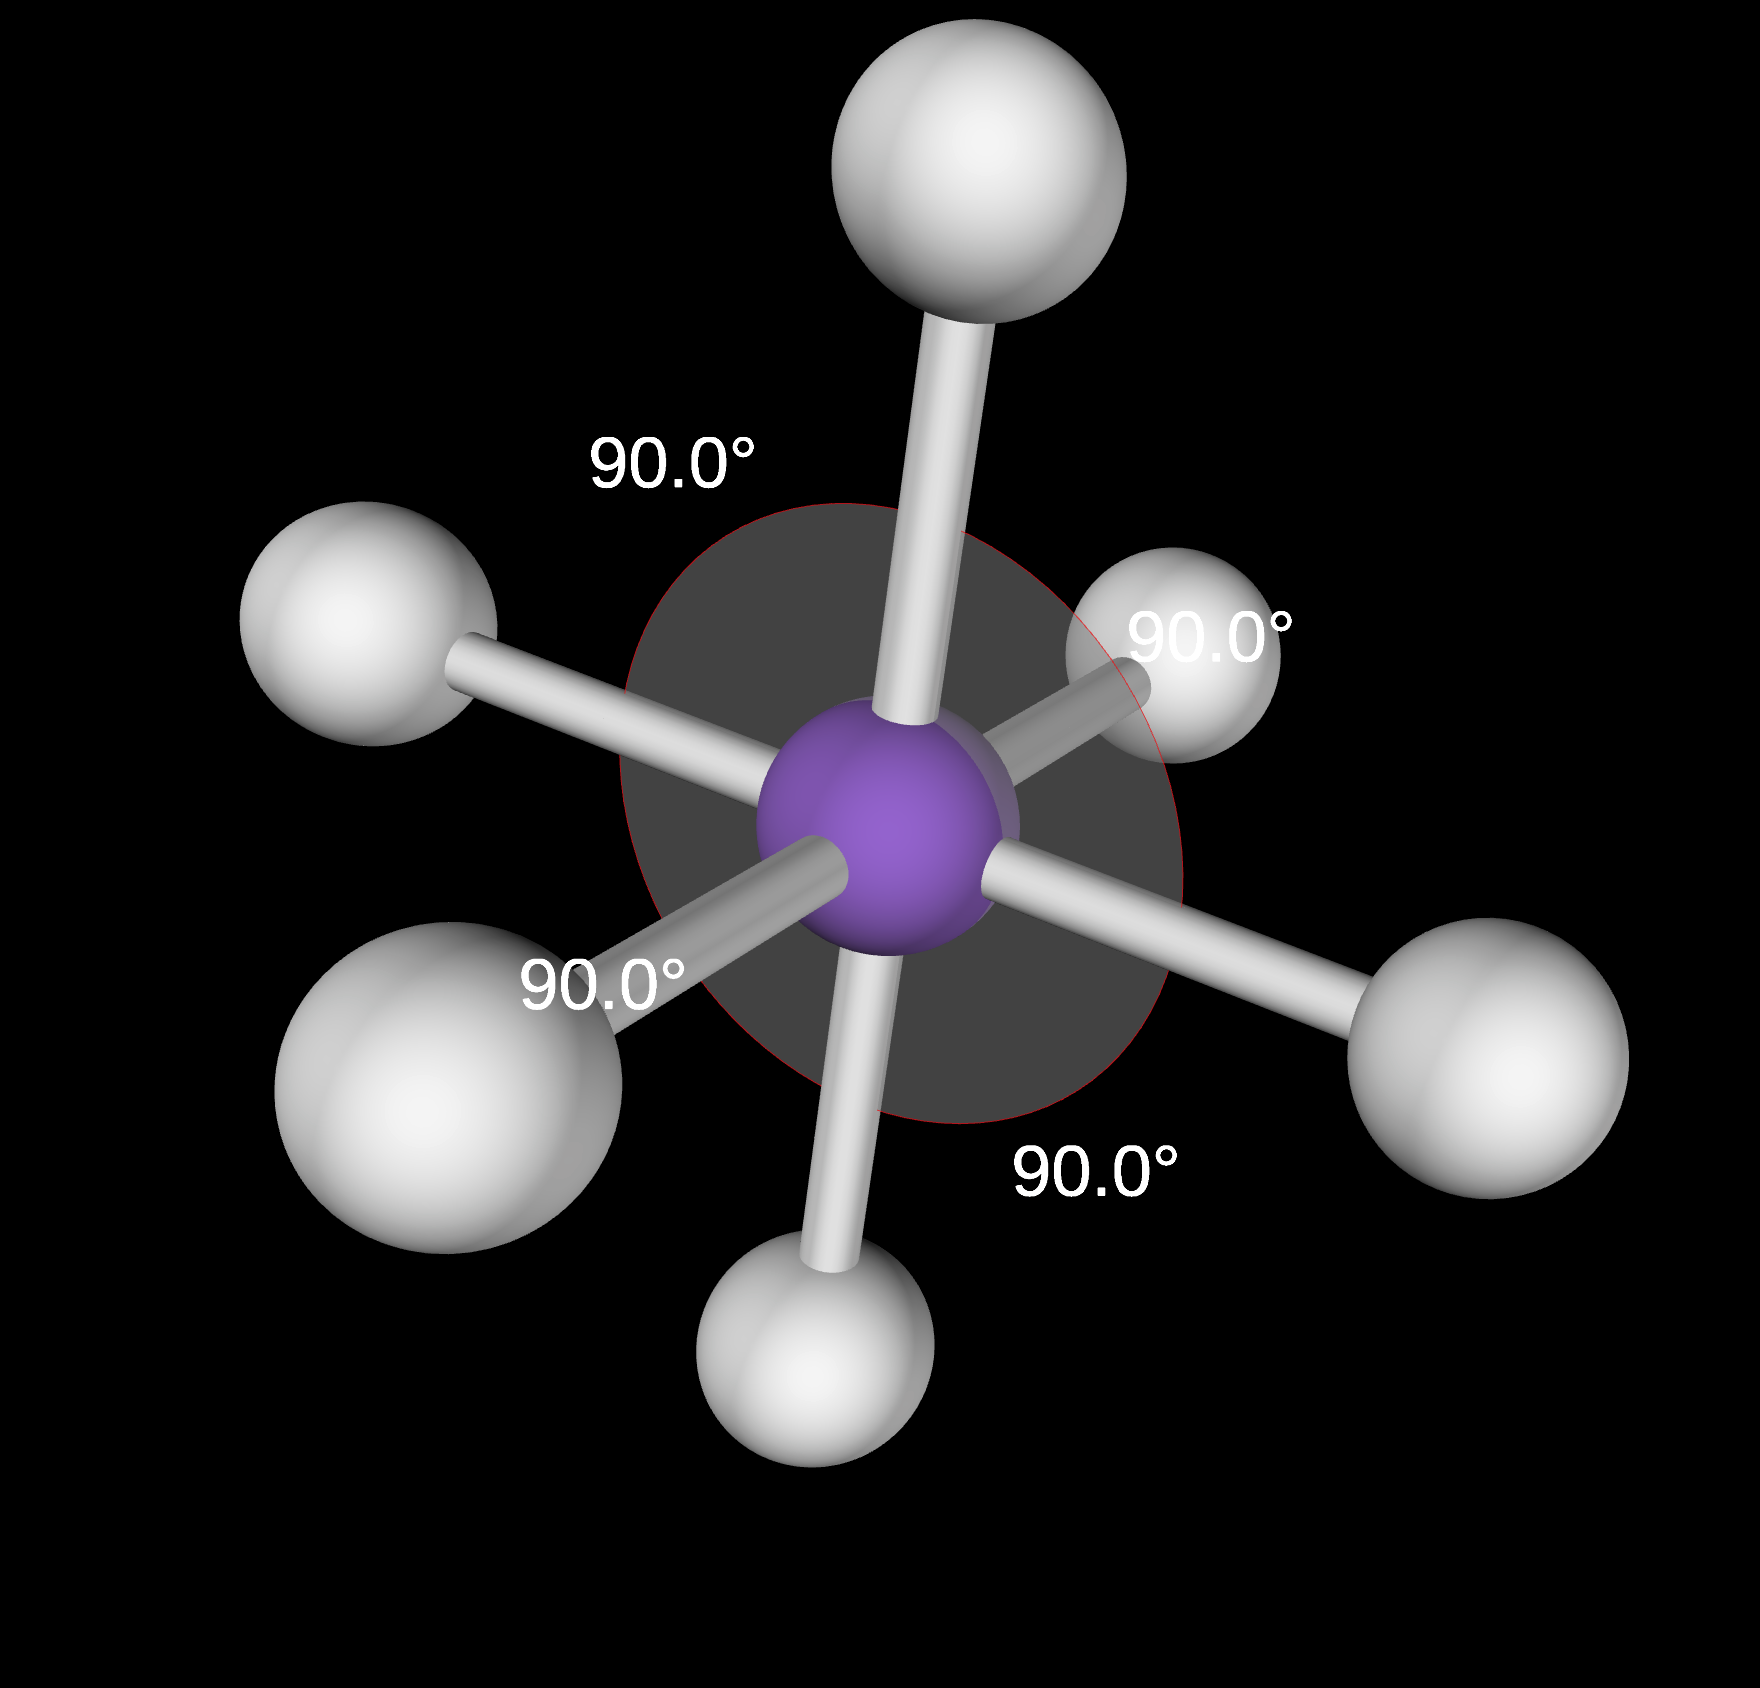
\includegraphics[width=0.4\textwidth]{Screenshot 2026-06-05 at 10.48.01 PM.png}
    \caption{Octahedral geometry with an octahedral electron domain geometry.}
\end{figure}
\subsubsection{Square Planar Molecular Geometry}
The square planar molecular geometry occurs when there are six electron pairs around the central atom, and four of them are bonding pairs while the other two are lone pairs. The bond angles in a square planar molecule are 90\textdegree  for all bonds. 
\begin{figure}[h]
    \centering
    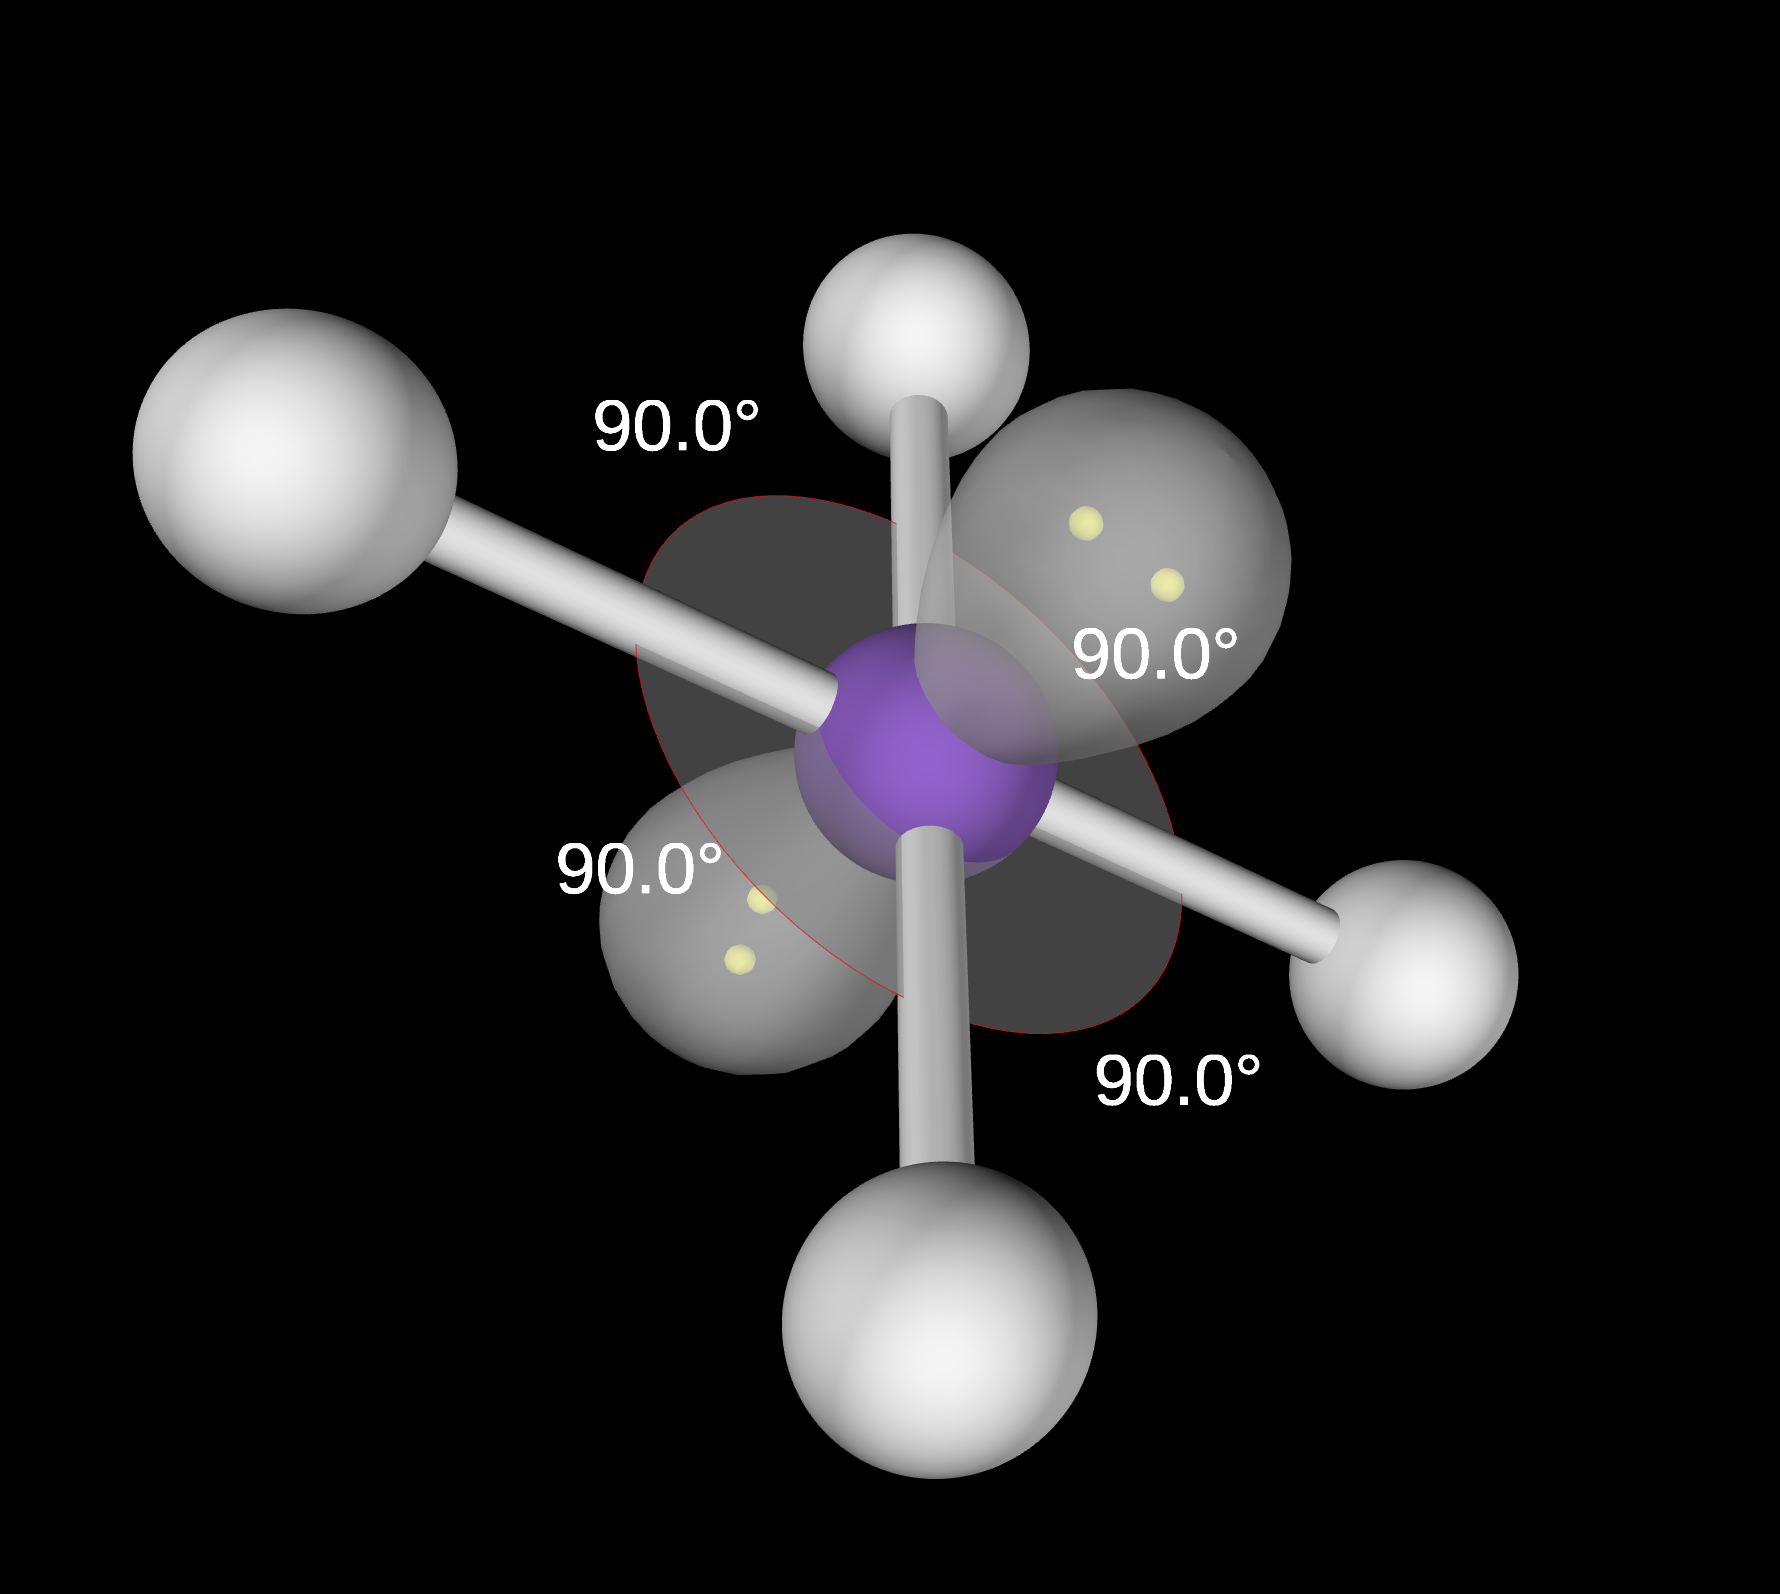
\includegraphics[width=0.4\textwidth]{Screenshot 2026-06-05 at 10.48.59 PM.png}
    \caption{Square planar geometry with an octahedral electron domain geometry.}
\end{figure}
\subsubsection{Molecular Geometry and Polarity}
The molecular geometry of a molecule can affect its polarity. A molecule is polar if it has a net dipole moment, which occurs when there is an uneven distribution of charge in the molecule. If a molecule has polar bonds but is symmetrical, the dipole moments can cancel out, resulting in a nonpolar molecule. 
\subsubsection{Valence Bond Theory}
Valence bond theory is a model used to describe the bonding in molecules based on the overlap of atomic orbitals. According to valence bond theory, a covalent bond forms when the atomic orbitals of two atoms overlap and the electrons in those orbitals are shared between the atoms. The strength of the bond depends on the extent of the overlap between the orbitals, with greater overlap resulting in a stronger bond. The bonding pair that forms between the nuclei of two atoms is called a sigma ($\sigma$) bond. When forming a double or triple bond, the additional bonds are called pi ($\pi$) bonds, which are formed by the side-to-side overlap of p orbitals. In order to make these bonds, atoms need to hybridize their orbitals to create new hybrid orbitals that can overlap more effectively. In this hybridized state, the atom has a lower energy and is more stable. The different hybridization states include $sp$, $sp^2$, and $sp^3$, which correspond to the number of electron pairs around the central atom and are linked to the electron domain geometry of the molecule.
\begin{table}[h]
    \centering
    \begin{tabular}{|c|c|c|}
        \hline
        Hybridization & \ce{e-} Pairs & Geometry \\
        \hline
        $sp$ & 2 & Linear \\
        $sp^2$ & 3 & Trigonal Planar \\
        $sp^3$ & 4 & Tetrahedral \\
        $sp^3d$ & 5 & Trigonal Bipyramidal \\
        $sp^3d^2$ & 6 & Octahedral \\
        \hline
    \end{tabular}
    \caption{Relationship between hybridization, number of electron pairs, and geometry.}
\end{table}
\subsubsection{Molecular Orbital Theory}
Molecular orbital theory is a model used to describe the bonding in molecules based on the combination of atomic orbitals to form molecular orbitals. According to molecular orbital theory, when two atoms come together to form a molecule, their atomic orbitals combine to form new molecular orbitals that are delocalized over the entire molecule. These orbitals are represented with diagrams that show the energy levels of the orbitals and the number of electrons in each orbital. 
\begin{figure}[h]
    \centering
    \begin{modiagram}[style=square,labels,names,AO-width=8pt,labels-fs=\footnotesize]
        \atom[\ce{H_a}]{right}{
            1s = {;up}
        }
        \atom[\ce{H_b}]{left}{
            1s = {;up}
        }
        \molecule[\ce{H2}]{
            1sMO = {;pair}
        }
\EnergyAxis
\end{modiagram}
\caption{Molecular orbital diagram of \ce{H2}.}
\end{figure}
There are three types of molecular orbitals: bonding, antibonding, and nonbonding. Bonding orbitals are lower in energy than the original atomic orbitals, antibonding orbitals are higher in energy than the original atomic orbitals, and nonbonding orbitals have the same energy as the original atomic orbitals. The electrons in a molecule will fill the molecular orbitals in order of increasing energy, following the Pauli exclusion principle and Hund's rule. 
\begin{figure}[h]
    \centering
    \begin{modiagram}[style=square,labels,names,AO-width=8pt,labels-fs=\footnotesize]
        \atom[\ce{He_a}]{right}{
            1s = {;pair}
        }
        \atom[\ce{He_b}]{left}{
            1s = {;pair}
        }
        \molecule[\ce{He2}]{
            1sMO = {;pair,pair},
            color = { 1sigma*=red }
        }
        
\EnergyAxis
\end{modiagram}
\caption{Molecular orbital diagram of \ce{He2}.}
\label{fig:he2MO}
\end{figure}
In figure \ref{fig:he2MO}, we see that the \ce{He2} molecule has two electrons in the bonding orbital and two electrons in the antibonding orbital, resulting in a bond order of zero and making the molecule unstable. This is why \ce{He2} does not exist under normal conditions.

To figure out the bond order of a molecule, we can use the formula:
\begin{equation}\label{eq:bondOrder}
    \text{Bond Order} = \frac{1}{2} \times (\ce{e-}_\text{bonding} - \ce{e-}_\text{antibonding})
\end{equation}
\begin{figure}[h]
    \centering
    \begin{modiagram}[style=square,labels,names,AO-width=8pt,labels-fs=\footnotesize]
        \atom[\ce{O_a}]{left}{
            1s, 2s, 2p = {;pair,up,up}
        }
        \atom[\ce{O_b}]{right}{
            1s, 2s, 2p = {;pair,up,up}
        }
        \molecule[\ce{O2}]{
            1sMO, 2sMO, 2pMO = {;pair,pair,pair,up,up},
            color = { 2piy*=red, 2piz*=red }
        }
        \EnergyAxis
    \end{modiagram}
    \caption{Molecular orbital diagram of \ce{O2}.}
\end{figure}
\section{States of Matter}
Matter has several phases, or states where particles exhibit a distinct set of properties. The three main phases of matter, in order of increasing entropy, are solids, liquids, and gases. These three, in addition to aqueous solutions, are the states of matter that are required for the AP exam. Another state of matter that is worth mentioning is plasma, which is a highly ionized gas that exists at extremely high temperatures, such as in stars. 
\begin{figure}[ht]
    \centering
    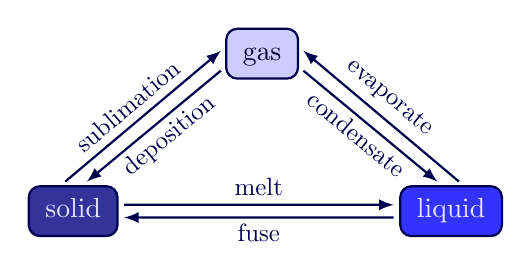
\begin{tikzpicture}[arrow/.style={->,thick,mydarkblue,shorten <=2,shorten >=2},
                            box/.style={thick,rounded corners=4,inner xsep=6,inner ysep=3}]
        \message{Phase transitions^^J}
        
        \node[blue!10!white,draw=mydarkblue,fill=blue!50!gray!80!black,box] (S) at (-2.4,0) {\strut solid};
        \node[blue!10!white,draw=mydarkblue,fill=blue!80!white,box] (L) at (2.4,0) {\strut liquid};
        \node[blue!20!black,draw=mydarkblue,fill=blue!20!white,box] (G) at (0,2) {\strut gas};
        
        \draw[arrow,->] (S.8) -- (L.173) node[above,midway,scale=0.9] {melt};
        \draw[arrow,->] (L.-173) -- (S.-8) node[below=-1pt,midway,scale=0.9] {fuse};
        
        \draw[arrow,->] (S.115) -- (G.-190) node[left=2pt,above,midway,sloped,scale=0.9] {sublimation};
        \draw[arrow,->] (G.-160) -- (S.70) node[left=-2pt,below=-1pt,midway,sloped,scale=0.9] {deposition};
        
        \draw[arrow,->] (L.65) -- (G.10) node[left=2pt,above,midway,sloped,scale=0.9] {evaporate};
        \draw[arrow,->] (G.-20) -- (L.110) node[left=2pt,below=-1pt,midway,sloped,scale=0.9] {condensate};
        
    \end{tikzpicture}
    \caption{Phase transitions between solids, liquids, and gases.}
    \label{fig:phase_transitions}
\end{figure}
There are several terms that should be mentioned relating to the process of changing states of matter. The process of changing from a solid to a liquid is called melting, while the reverse process is called freezing. The process of changing from a liquid to a gas is called vaporization, while the reverse process is called condensation. The process of changing directly from a solid to a gas is called sublimation, while the reverse process is called deposition.
\subsection{Phase Diagrams}
A phase diagram is a graphical representation of the different phases of a substance as a function of temperature and pressure. The phase diagram of a substance shows the conditions under which the substance exists as a solid, liquid, or gas. The lines on the phase diagram represent the conditions under which two phases coexist in equilibrium, at which point is the phase change occurs. 
\begin{figure}[ht]
    \centering

    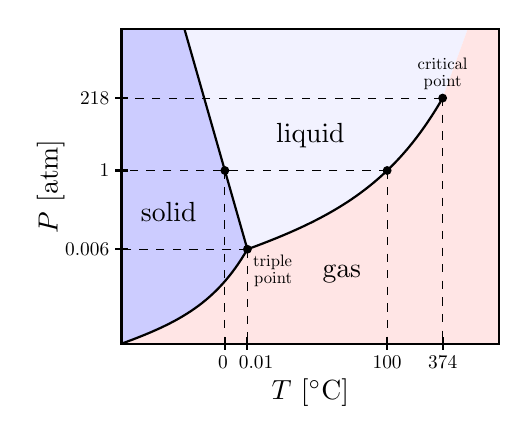
\begin{tikzpicture}[scale=0.4]
        \message{Phase diagrams^^J}
        
        \def\xtick#1#2{\draw[thick] (#1)++(0,.2) --++ (0,-.4) node[below=-.5pt,scale=0.7] {#2};}
        \def\ytick#1#2{\draw[thick] (#1)++(.2,0) --++ (-.4,0) node[left=-.5pt,scale=0.7] {#2};}
        
        % COORDINATES
        \coordinate (O) at (0,0);
        \coordinate (N1) at (2,10);
        \coordinate (N2) at (11,10);
        \coordinate (NE) at (12,10);
        \coordinate (NW) at (0,10);
        \coordinate (SE) at (12,0);
        \coordinate (W) at (0,5);
        \coordinate (S) at (6,0);
        \coordinate (C) at (10.2,7.8); % critical
        \coordinate (T) at (4,3); % triple
        
        % PATHS
        \def\SL{(T) -- (N1)}
        \def\SG{(O) to[out=20,in=-120] (T)}
        \def\LG{(T) to[out=20,in=-120] (C)}
        \def\atm{(0,5.5) -- (12,5.5)}
        \path[name path=SL] \SL;
        \path[name path=LG] \LG;
        \path[name path=atm] \atm;
        
        % REGIONS
        \fill[mylightblue] \SG -- (N1) -- (NW) -- cycle;
        \fill[blue!5] \LG -- (N2) -- (N1) -- cycle;
        \fill[mylightred] \LG -- (N2) -- (NE) -- (SE) -- \SG -- cycle;
        \node at (1.5,4.2) {solid};
        \node at (7,2.2) {gas};
        \node at (6,6.6) {liquid};
        
        %% MIXED
        %\shade[top color=mylightblue,bottom color=mylightred,shading angle=70]
        %  (10.4,7.7) -- (11.2,10) -- (10.8,10) -- (10.0,7.7) -- cycle;
        
        % POINTS
        \fill[black,name intersections={of=SL and atm,by=M}] (M) circle (4pt);
        \fill[black,name intersections={of=LG and atm,by=B}] (B) circle (4pt);
        \fill (T) circle (4pt) node[below right,scale=0.6,align=right] {triple\\[-2pt]point};
        \fill (C) circle (4pt) node[above=1pt,scale=0.6,align=center] {critical\\[-2pt]point};
        
        % LINES
        \draw[thick] \SG;
        \draw[thick] \LG;
        \draw[thick] \SL;
        \draw[dashed] (M) -- ($(M |- 0,0)$) coordinate (Mx);
        \draw[dashed] (T) -- ($(T |- 0,0)$) coordinate (Tx);
        \draw[dashed] (T) -- ($(T -| 0,0)$) coordinate (Ty);
        \draw[dashed] (B) -- ($(B |- 0,0)$) coordinate (Bx);
        \draw[dashed] (B) -- ($(B -| 0,0)$) coordinate (By);
        \draw[dashed] (C) -- ($(C |- 0,0)$) coordinate (Cx);
        \draw[dashed] (C) -- ($(C -| 0,0)$) coordinate (Cy);
        
        % AXES
        \draw[thick] (O) rectangle (NE);
        \node[left=17pt,above,rotate=90] at (W) {$P$ [atm]};
        \node[below=9pt] at (S) {$T$ [\si{\degree C}]};
        \xtick{Mx}{\hspace{-2pt}0}
        \xtick{Tx}{\hspace{9pt}0.01}
        \ytick{Ty}{0.006}
        \xtick{Bx}{100}
        \ytick{By}{1}
        \xtick{Cx}{374}
        \ytick{Cy}{218}
        
    \end{tikzpicture}
    \caption{Phase diagram of water.}
    \label{fig:phase_diagram}
\end{figure}
The point where all three phases coexist in equilibrium is called the triple point, and the point where the liquid and gas phases become indistinguishable is called the critical point. The curve between liquids and gases is called the vapor-pressure curve, and the curve between solids and liquids is called the melting curve. The normal melting point and normal boiling point of a substance are the points on the phase diagram where the melting curve and vapor-pressure curve intersect with the line of 1 atm pressure, respectively.
\subsection{Gases}
Gasses are the most entropic phase of matter and are characterized by their low density, little intermolecular attraction between particles, connection with pressure, and their higher potential energy. These properties allow gases to assume both the volume and shape of their container, and to be easily compressed. They flow easily and diffuse quickly. 
\subsubsection{Pressure}
An important topic to discuss in relationship to gases is pressure. Pressure is defined as the amount of force per unit of area.
\begin{equation}\label{eq:pressure}
    P = \frac{F}{A}
\end{equation}
The pressure we experience on Earth is caused by the weight of the air above us. In the context of gases, pressure is caused by the collisions of gas particles between the walls and each other. The more collisions there are, the higher the pressure. 

We can measure pressure using tools such as a barometer, which measures atmospheric pressure, and a manometer, which is used to compare the unknown pressure of a gas to a known pressure, such as atmospheric pressure. Both of these tools work by measuring the height of a column of a liquid, usually mercury, that is supported by the pressure of the gas. The height of the column is directly proportional to the pressure of the gas. 

There are many units of pressure, but the most common ones are atmospheres (atm), millimeters of mercury (mmHg), and pascals (Pa). The standard SI unit of pressure is the pascal, and is defined as one newton per square meter. Usually, a pascal is too small to be used in real world problems, and instead kilopascals (kPa) or bars are used. Where 1 kPa is equal to 1000 Pa, and 1 bar is equal to 100 kPa. Millimeters of mercury, sometimes called torr, is a unit of pressure that is based on the height of a column of mercury that is supported by the pressure of the gas. This is an older unit that originally came from the use of mercury barometers, but is still commonly used today. Atmospheres is a unit of pressure that is based on the average atmospheric pressure at sea level, which is approximately 101.325 kPa or 760 mmHg.
\subsubsection{Standard Temperature and Pressure}
Standard temperature and pressure (STP) is a set of conditions that are commonly used in gas law problems. STP is defined as a temperature of 0\textdegree C (273.15 K) and a pressure of 1 atm (101.325 kPa or 760 mmHg). These conditions are different from the standard conditions used in thermodynamics problems.
\subsubsection{Gas Laws}
Gas laws are mathematical relationships that describe the interaction between four variables of a gas: pressure, volume, temperature, and number of moles. These laws apply to all ideal gases and tell us how gases behave. The relationships between these variables all have different names based on the variables involved, and in many cases the scientist who discovered the relationship. 
The first gas law is Boyle's Law, which describes the relationship between pressure and volume.
\begin{equation}\label{eq:boyle}
    P \propto \frac{1}{V}
\end{equation}
The next gas law is Charles's Law, which describes the relationship between volume and temperature.
\begin{equation}\label{eq:charles}
    V \propto T
\end{equation}
The next gas law is Gay-Lussac's Law, which describes the relationship between pressure and temperature.
\begin{equation}\label{eq:gaylussac}
    P \propto T
\end{equation}
The next gas law is Avogadro's Law, which describes the relationship between volume and number of moles.
\begin{equation}\label{eq:avogadro}
    V \propto n
\end{equation}
Combining Boyle's Law, Charles's Law, and Gay-Lussac's Law gives us the Combined Gas Law, which describes the relationship between pressure, volume, and temperature.
\begin{equation}\label{eq:combined}
    \frac{PV}{T} = k
\end{equation}
Where $k$ is a constant. 
Finally, combining the Combined Gas Law with Avogadro's Law gives us the Ideal Gas Law, which describes the relationship between pressure, volume, temperature, and number of moles.
\begin{equation}\label{eq:ideal}
    PV = nRT
\end{equation}
Where $R$ is the ideal gas constant, which has a value of $0.0821 \, \text{L·atm·K}^{-1}\text{·mol}^{-1}$. This constant also appears in some thermodynamics equations, such as the conversion between Gibbs free energy and the equilibrium constant \eqref{eq:free_energy_equilibrium}, in which case we use the value of $R$ in joules per mole per kelvin, which is $8.314 \, \text{J·K}^{-1}\text{·mol}^{-1}$.
Using this equation, we can rearrange the variables to relate the molar mass of a gas to its density, pressure, and temperature.
\begin{equation}\label{eq:molar_mass}
    M = \frac{\rho RT}{P}
\end{equation}
Where $\rho$ is the density of the gas. 
In addition to the ideal gas law, another law of gases is Dalton's Law of Partial Pressures, which states that the total pressure of a gas mixture is equal to the sum of the partial pressures of each individual gas in the mixture.
\begin{equation}\label{eq:dalton}
    P_{total} = P_1 + P_2 + \dots + P_n
\end{equation}
Where $P_{total}$ is the total pressure of the gas mixture, and $P_1$, $P_2$, ..., $P_n$ are the partial pressures of each individual gas in the mixture. 
\subsubsection{Mole Fraction}
The mole fraction of a gas is the ratio of the number of moles of that gas to the total number of moles of all gases in the mixture. Using the mole fraction, we can relate the partial pressure of a gas to its mole fraction and the total pressure of the gas mixture. This can also be used along with Dalton's Law of Partial Pressures to convert between the mole fraction of a gas and its partial pressure.
\subsubsection{Real Gases}
The main gas laws assume that gases behave ideally, assuming that atoms or molecules do not take up space, interact with each other, and that kinetic energy is directly proportional to temperature. In reality, this is not the case as real gases do exhibit these properties. The ideal gas law is a good approximation for real gases at low pressures and high temperatures, where the particles are far apart and have little interaction with each other. However, at high pressures and low temperatures, the ideal gas law breaks down. A correction for these properties is given by the Van der Waals equation, which is a modified version of the ideal gas law that takes into account the volume of the gas particles and the intermolecular forces between them. The Van der Waals equation is given by:
\begin{equation}\label{eq:vanderwaals}
    \left(P + \frac{an^2}{V^2}\right)(V - nb) = nRT
\end{equation}
Where $a$ is a measure of the strength of the intermolecular forces between the gas particles, and $b$ is a measure of the volume of the gas particles. The values of $a$ and $b$ are specific to each gas and can be found in tables.
\subsubsection{Effusion and Diffusion}
Effusion is the process of a gas passing through a tiny opening, while diffusion is the process of a gas spreading out and mixing with other gases. The rate of effusion and diffusion of a gas is related to its molar mass, with lighter gases effusing and diffusing faster than heavier gases.
This relationship is given by Graham's Law, which states that the rate of effusion or diffusion of a gas is inversely proportional to the square root of its molar mass.
\begin{equation}\label{eq:graham}
    \frac{r_1}{r_2} = \sqrt{\frac{M_2}{M_1}}
\end{equation}
Where $r_1$ and $r_2$ are the rates of effusion or diffusion of gases 1 and 2, and $M_1$ and $M_2$ are the molar masses of gases 1 and 2. This equation is not required for calculations on the AP exam, but its concept is required.
\subsection{Liquids}
Liquids are the middle ground between solids and gases, where intermolecular forces are strong enough to hold the particles together, but not strong enough to keep them in a fixed position. This phase is relatively rare in reality as most substances exist as either solids or gases at room temperature, but has a lot of interesting properties. Water is one of the most common liquids and has many unique properties that are important to understand in chemistry. 

Compared to gases which are $>99\%$ empty space, or solids which are $<0.1\%$ empty space, liquids are in the middle with about $10\%$ empty space. They are able to assume the shape of their container, but have a fixed volume. They are relatively incompressible, and flow easily similarly to gases. Both liquids and gases are fluids, which means they can flow and take the shape of their container. 
\subsubsection{Intermolecular Forces}
The second law of thermodynamics states that the entropy of the universe always increases, which means that systems will naturally tend towards disorder. This would suggest that all mater should exist as a gas, which is the most entropic phase of matter. However, this is not the case as there are intermolecular forces that hold particles together and prevent them from existing as a gas. 

Intramolecular forces are the forces that hold atoms together within a molecule, the chemical bonds that make up molecules. Intermolecular forces are the forces that hold molecules together, and are responsible for the properties of liquids and solids. Compared to intramolecular forces, intermolecular forces are much weaker, but they are still strong enough to hold molecules together and prevent them from existing as a gas. Where intramolecular forces affect the chemical properties of a substance, intermolecular forces affect the physical properties of a substance, such as its boiling point, melting point, vapor pressure, and viscosity. In equation \eqref{eq:vanderwaals}, we included a term to account for the intermolecular forces between gas particles, which is the $an^2/V^2$ term. 

There are four main types of intermolecular forces: Ion-dipole forces, dipole-dipole forces, hydrogen bonding, and London dispersion forces. Van der Waals forces is a term that is used to refer to the final three types of intermolecular forces.
\subsubsection{Ion-Dipole Forces}
Ion-dipole forces are the strongest of the four, and occur between an ion and a polar molecule. This force comes from the electrostatic attraction between the charged ion and the partial charges on the polar molecule. 

This is most commonly seen in aqueous solutions, where the positive and negative ions of a solute are attracted to the partial charges on the water molecules. 

These forces are the strongest of the four.

\subsubsection{Dipole-Dipole Forces}
Dipole-dipole forces occur between two polar molecules, and come from the electrostatic attraction between the partial positive charge on one molecule and the partial negative charge on the other molecule. 


\subsubsection{Hydrogen Bonding}
Hydrogen bonding is a special type of dipole-dipole force that occurs when a hydrogen atom is bonded to a highly electronegative atom, such as nitrogen, oxygen, or fluorine. This creates a strong dipole moment, and the hydrogen atom can form a strong attraction with the lone pair of electrons on another molecule. These bonds are stronger than regular dipole-dipole forces, but still weaker than ion-dipole forces.
There increased strength in comparison to regular dipole-dipole forces comes from the very small size of the hydrogen atom, which allows it to get very close to the electronegative atom and form a strong attraction. 

The presence of hydrogen bonding in water is responsible for many of its unique properties, such as its high boiling point, high specific heat capacity, and high surface tension. 
\subsubsection{London Dispersion Forces}
London dispersion forces are the weakest of the four, and occur between all molecules, whether they are polar or nonpolar. These forces come from uneven arrangements of electrons around a molecule, which creates temporary dipoles that can induce dipoles in neighboring molecules. The strength of London dispersion forces increases with the size of the molecule, as larger molecules have more electrons and a greater surface area for interactions.
\subsubsection{IMF and Boiling Point}
The more intermolecular forces a substance has, the higher its boiling point will be. This is because more energy is required to overcome the intermolecular forces and convert the substance from a liquid to a gas. This is why the boiling point of the alkanes increases as the number of carbons increases, as the larger alkanes have more electrons and a greater surface area for London dispersion forces to occur. This is also why water has a much higher boiling point than other molecules of similar size, as it has strong hydrogen bonding in addition to London dispersion forces.
\subsubsection{Vapor Pressure}
Vapor pressure is the pressure exerted by the gas released by a liquid when it is in equilibrium with its vapor. Both evaporation and condensation occur at the surface of a liquid, and when the rate of evaporation equals the rate of condensation, the system is in dynamic equilibrium. At this point, the pressure exerted by the gas released by the liquid is called the vapor pressure. The vapor pressure of a liquid depends on the strength of the intermolecular forces in the liquid, and the temperature of the liquid. The relationship between vapor pressure and temperature is given by the Clausius-Clapeyron equation, which describes how the vapor pressure of a liquid changes with temperature.
\begin{equation}\label{eq:clausius}
    \ln P = -\frac{\Delta H_{vap}}{RT} + C
\end{equation}
Where $P$ is the vapor pressure and $\Delta H_{vap}$ is the enthalpy of vaporization.
This equation can be rearranged to showcase the change in vapor pressure with a change in temperature.
\begin{equation}\label{eq:clausius_rearranged}
    \ln \frac{P_2}{P_1} = -\frac{\Delta H_{vap}}{R}\left(\frac{1}{T_2} - \frac{1}{T_1}\right)
\end{equation}

The reason that such an equilibrium exists is because the particles at the surface of a liquid have enough energy to overcome the intermolecular forces and escape into the gas phase, which can be seen in the Maxwell-Boltzmann distribution of particle energies (\ref{fig:MaxwellBoltzmann}), where the particles with the highest energies are able to escape the liquid and become a gas. We can also represent a phase change as a reaction, which has its own equilibrium constant, which is related to the pressure of the gas released by the liquid. 
\subsubsection{Viscosity}
Viscosity is a measure of a liquid's resistance to flow. It is determined by the strength of the intermolecular forces in the liquid, as well as the size and shape of the molecules.
\subsubsection{Surface Tension}
The surfaces of liquids are stronger and have more tension than the rest of the liquid, which is caused by the imbalance of intermolecular forces at the surface. This surface tension allows liquids to form droplets and to resist external forces, such as gravity. 
\subsubsection{Capillary Action}
Capillary action is the ability of a liquid to flow in narrow spaces without the assistance of external forces. This is caused by the combination of cohesive forces between the liquid molecules and adhesive forces between the liquid molecules and the surface of the narrow space. This is why water can climb up a thin tube.
\subsubsection{Water and its Unique Properties}
Water has several unique properties due to its hydrogen bonding, including a high specific heat capacity, high heat of vaporization, and the ability to dissolve many substances. These properties are essential for life and influence many natural processes. Its properties allow it to be one of the best solvents, as it can dissolve a wide variety of substances, including ionic compounds and polar molecules. 
\subsubsection{Liquid Crystals}
Liquid crystals are a state of matter that has properties of both liquids and solids. They have an ordered structure like solids, but can flow like liquids. They are used in many applications, such as in computer screens and displays. Nematic liquid crystals have molecules that are oriented in the same direction, while smectic liquid crystals have molecules that are arranged in layers. Cholesteric liquid crystals have molecules that are arranged in a helical pattern.
\subsection{Solids}
Having the least amount of entropy, solids are the most ordered phase of matter. They have strong intramolecular and intermolecular forces that hold the particles together in a fixed position, giving solids a definite shape and volume. Even with this rigid structure they still have small vibrations of the particles. They tend to form either crystalline or amorphous structures, where crystalline solids have a regular repeating pattern of particles, while amorphous solids do not have a regular pattern. 
\subsubsection{Amorphous Solids}
Solids such as glass, rubber, and plastic all lack a regular repeating pattern of particles, and are classified as amorphous solids. Consequently, their structures are not as rigid, and no internal geometry. They have comparatively lower IMFs compared to crystalline solids.
\subsubsection{Crystalline Solids}
Crystalline solids have a regular repeating pattern of particles, and have four main types: ionic, covalent network, metallic, and molecular. 

In ionic solids, the unit particles are positive and negative ions that are held together by electrostatic attraction. These solids are hard and brittle, have high melting points, and are poor conductors of heat and electricity. Salts (\ce{NaCl} or \ce{Ca(NO3)2}) and other ionic compounds are examples of ionic solids.

In covalent network solids, the unit particles are atoms connected by a network of covalent bonds which hold the particles together. They are very hard, have very high melting points, and are often poor conductors of heat and electricity. Diamond (\ce{C}) and quartz (\ce{SiO2}) are examples of covalent network solids. Covalent network solids can also be further classified into two dimensional solids and three dimensional solids. 

Metallic solids have a lattice of metal atoms connect with metallic bonds. The demoralized electrons cause metallic solids to be very good conductors of heat and electricity, and they are malleable and ductile. Their hardness and melting points can vary widely. Examples of metallic solids include iron (\ce{Fe}), copper (\ce{Cu}), and aluminum (\ce{Al}).

Molecular solids have atoms or molecules as their unit particles, which are held together by intermolecular forces. They are generally soft, have low to moderate melting points, and are poor conductors of heat and electricity. Examples include sugar (\ce{C12H22O11}), or dry ice (\ce{CO2}). Molecular solids can also be further classified into polar, nonpolar, and hydrogen bonding solids, based on the types of intermolecular forces that hold the particles together.
\subsubsection{Crystal Lattices and Unit Cells}
A crystal lattice is a three-dimensional arrangement of atoms, ions, or molecules in a crystalline solid. The unit cell of a lattice is the smallest repeating unit that shows the entire structure's symmetry and properties. There are seven main types of crystal lattices: cubic, tetragonal, orthorhombic, rhombohedral, hexagonal, monoclinic, and triclinic. The only one relevant to the AP exam is the cubic lattice, which has three subtypes: simple cubic, body-centered cubic, and face-centered cubic. 
\begin{figure*}[ht]
    \centering
    \begin{subfigure}{0.3\textwidth}
        \centering
        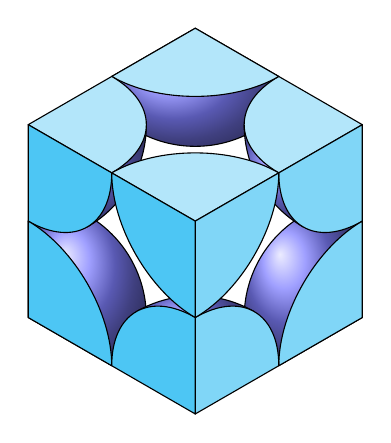
\begin{tikzpicture}[isometric view,rotate around z=180,line cap=round,line join=round]
           \def\a{3} % edge length
            \pgfmathsetmacro\r{0.5*\a} % sphere radius
            % background
            \foreach\i in {0,120,240}
            \draw[rotate=\i,my ball] (\a,0,0) --++ (0,\r,0) arc (90:135:\r) arc (0:60:\r cm)
                {[canvas is xz plane at y=0] arc (135:90:\r)} -- cycle;
            % foreground
            \foreach\i in {0,120,240}
            \draw[rotate=\i,my ball] (\a,\a,0) --++ (60:\r cm) arc (60:120:\r cm) -- cycle;
            % section planes
            \foreach\s in {xy,xz,yz} \foreach\i in {1,...,4}
            \draw[\s,rotate=90*\i] (45:{\a*sin(45)}) --++ (180:\r) arc (180:270:\r) -- cycle;
        \end{tikzpicture}
        \caption{Simple cubic unit cell.}
        \label{fig:simple_cubic}
    \end{subfigure}
    \begin{subfigure}{0.3\textwidth}
        \centering
        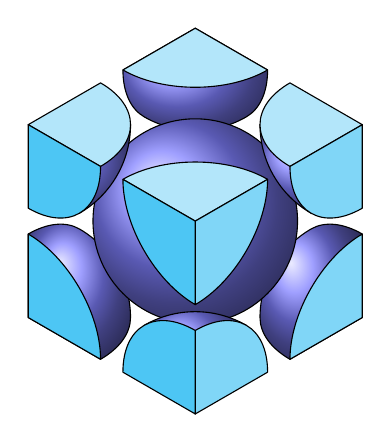
\begin{tikzpicture}[isometric view,rotate around z=180,line cap=round,line join=round]
            \def\a{3} % edge length
            \pgfmathsetmacro\r{0.25*sqrt(3)*\a} % sphere radius
            % background
            \foreach\i in {0,120,240}
            \draw[rotate=\i,my ball] (\a,0,0) --++ (0,\r,0) arc (90:135:\r) arc (0:60:\r cm)
                {[canvas is xz plane at y=0] arc (135:90:\r)} -- cycle;
            % sphere (center)
            \draw[my ball]  (0.5*\a,0.5*\a,0.5*\a) circle (\r cm);
            % foreground
            \foreach\i in {0,120,240}
            \draw[rotate=\i,my ball] (\a,\a,0) --++ (60:\r cm) arc (60:120:\r cm) -- cycle;
            % section planes
            \foreach\s in {xy,xz,yz} \foreach\i in {1,...,4}
            \draw[\s,rotate=90*\i] (45:{\a*sin(45)}) --++ (180:\r) arc (180:270:\r) -- cycle;
        \end{tikzpicture}
        \caption{Body-centered cubic unit cell.}
        \label{fig:body_centered_cubic}
    \end{subfigure}
    \begin{subfigure}{0.3\textwidth}
        \centering
        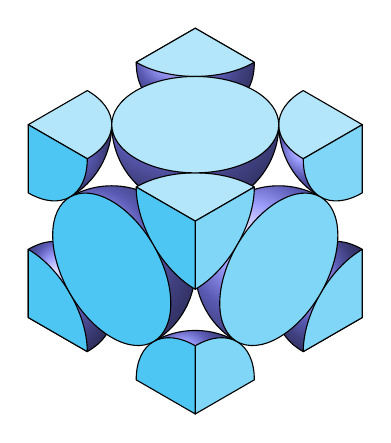
\begin{tikzpicture}[isometric view,rotate around z=180,line cap=round,line join=round]
                    \def\a{3} % edge length
                    \pgfmathsetmacro\r{0.25*sqrt(2)*\a} % sphere radius
                    % background
                    \foreach\i in {0,120,240}
                    \draw[rotate=\i,my ball] (\a,0,0) --++ (0,\r,0) arc (90:135:\r) arc (0:60:\r cm)
                        {[canvas is xz plane at y=0] arc (135:90:\r)} -- cycle;
                    % foreground
                    \foreach\i in {0,120,240}
                    \draw[rotate=\i,my ball] (\a,\a,0) --++ (60:\r cm) arc (60:120:\r cm) -- cycle;
                    \foreach\i in {0,120,240}{
                    \begin{scope}[rotate=\i]
                    \clip (0.5*\a,0,0) --++ (0,-\r,\r) -- (-0.5*\a,0.5*\a,0.5*\a) -- (0.5*\a,0.5*\a,-0.5*\a);
                    \draw[my ball] (0.5*\a,0,0) circle (\r cm);
                    \end{scope}}
                    % section planes
                    \foreach\s in {xy,xz,yz} \foreach\i in {1,...,4}
                    \draw[\s,rotate=90*\i] (45:{\a*sin(45)}) --++ (180:\r) arc (180:270:\r) -- cycle;
                    \foreach\s in {xy,xz,yz}
                    \draw[\s] (0,0) circle (\r cm);
        \end{tikzpicture}
        \caption{Face-centered cubic unit cell.}
        \label{fig:face_centered_cubic}
    \end{subfigure}
    \caption{The three types of cubic unit cells.}
    \label{fig:cubic_unit_cells}
\end{figure*}
In the simple cubic there is one atom at each corner of the cube, and the atoms touch each other along the edges of the cube. There is a total of one atom in the entire unit cell, as each corner only contains one-eigth of an atom as seen in figure \ref{fig:simple_cubic}.

In a body-centered cubic, there is one atom at each corner of the cube and one atom in the center of the cube. This results in a total of two atoms per unit cell, with one atom in the center, and another distributed among the eight corners as seen in figure \ref{fig:body_centered_cubic}.

A face-centered cubic has one atom at each corner of the cube and one atom in the center of each face of the cube. This results in a total of four atoms per unit cell, with three atoms distributed among the six faces, and one atom distributed among the eight corners as seen in figure \ref{fig:face_centered_cubic}.
\subsubsection{Ionic Solids Unit Cells}
When making unit cells for ionic solids, there are two equivelent methods, larger ions at the corners or smaller ions at the corners. In both the cation to anion ratio is the same for the crystal as for the molecular formula. In \ce{NaCl}, the chloride ions make a face-centered cubic while the smaller sodium ions fill in the gaps between the chloride ions. 
\subsubsection{Metal Alloys}
An alloy is a solid homogeneous mixture of two or more elements to gain specific properties. There are two main types of alloys: substitutional alloys and interstitial alloys. In a substitutional alloy, an atom of a similar size to the solvent atom is used to replace some of the solvent atom in the lattice structure. Bronze is an example of a substitutional alloy, which is made by replacing some of the copper atoms with tin atoms. In an interstitial alloy, smaller atoms are used to fill in the gaps between the solvent atoms in the lattice structure. Steel is an example of an interstitial alloy, which is made by filling in the gaps between iron atoms with carbon atoms. 
\subsubsection{Allotropes}
Allotropes are different forms of the same element that have different physical properties. Some elements like carbon can exist in multiple forms, such as diamond, graphite, and graphene. These different forms of carbon have different physical properties due to their different structures.
\subsubsection{Semiconductors}
Semiconductors are materials that have electrical conductivity between that of a conductor and an insulator. They are used in many electronic devices and are made through a process called dopeing where elements such as silicon or germanium are mixed with small amounts of other elements to change the conductivity. n-type semiconductors have more conductivity and p-type semiconductors have less conductivity. When you combine n-type and p-type semiconductors, you get a p-n junction, which is the basis for many electronic devices such as diodes and transistors.
\subsubsection{Foam}
Foam is a type of solid that is made up of a large number of gas bubbles trapped in a liquid or solid matrix. The process of making a foam starts with an emulsion, where monomers are a fuid, before foaming agents are added to create the gas bubbles. The foam is then solidified through a process called polymerization and you get a polymer foam. 
\subsection{Solutions}
Solutions are evenly distributed mixtures of substances that can not be easily separated. They are essential to many chemical reactions and processes. In all solutions there are one or more solutes dissolved in a solvent. These solutes can not be filtered out of the solvent but can be distilled using the different boiling points of substances. Solutes always stay mixed in a solvent and particles are always in motion. The solution has different properties than the solvent does alone which is why solutions are useful for reactions. Volumes of solutions are not always additive as the solute can fit into the spaces between the solvent particles. There are nine types of solution based on the phases of the solvent and solute. 
\begin{table}[ht]
    \centering
    \begin{tabularx}{\columnwidth}{|c|c|X|}
        \hline
        \textbf{Solvent} & \textbf{Solute} & \textbf{Example} \\
        \hline
        Gas & Gas & Air (Oxygen dissolved in Nitrogen)\\
        Gas & Liquid & Water vapor in air\\
        Gas & Solid & Particulates such as dust in air\\
        Liquid & Gas & Carbonated water (CO2 dissolved in water)\\
        Liquid & Liquid & Gasoline (a mixture of hydrocarbons)\\
        Liquid & Solid & Saltwater (NaCl dissolved in water)\\
        Solid & Gas & Hydrogen in palladium\\
        Solid & Liquid & Amalgam (Mercury dissolved in another metal)\\
        Solid & Solid & Alloys such as bronze (tin dissolved in copper)\\
        \hline
    \end{tabularx}
    \caption{Examples of solutions based on the phases of the solvent and solute.}
    \label{tab:solution_types}
\end{table}
\subsubsection{Solubility}
The main rule that most solutions follow when it comes to solubility is "like dissolves like," that is, polar solvents are able to dissolve polar solutes and non-polar solvents are able to dissolve non-polar solutes. The closer the polarities of the solvent and solute, the better the solubility. Conversely, substances with different polarities tend to not dissolve well. There are of course exceptions to this rule. We call substances that can dissolve in each other miscible, and substances that can not dissolve in each other immiscible.

Solubility itself is the maximum amount of a solute that can be dissolved in a solvent. This is typically represented in units of g/100mL for solids in liquids and mg/L for gases. The solubility of a substance can be affected by several factors. In order of decreasing importance they are polarity, materials, temperature, and pressure. If the solubility of a substance is very low we call it insoluble. 

We can represent the solubility of a substance at different temperatures using a solubility curve. 
\begin{figure}[ht]
    \centering
    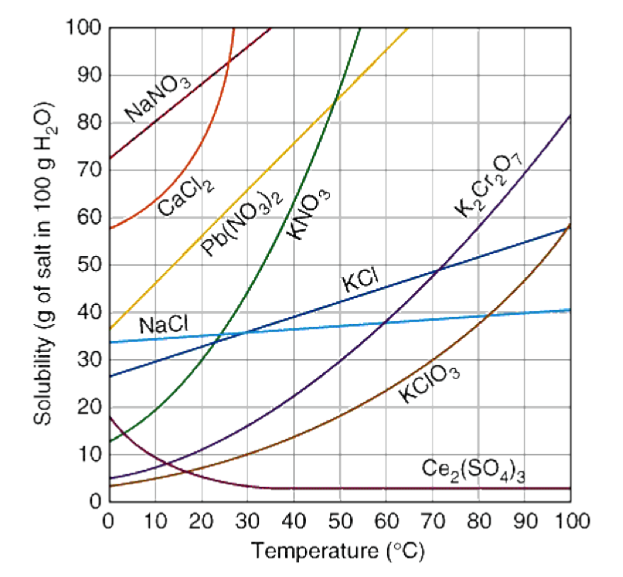
\includegraphics[width=0.9\columnwidth]{solubility-curve-solid.png}
    \caption{Solubility curve of \ce{NaNO3}, \ce{CaCl2}, \ce{Pb(NO3)2}, \ce{NaCl}, \ce{KCl}, \ce{K2Cr2O7}, \ce{KClO3}, and \ce{Ce2(SO4)3} in water.}
    \label{fig:solubility_curve}
\end{figure}

A solution is saturated when it contains the maximum amount of solute that can be dissolved in the solvent at a given temperature, or it lies on the solubility curve. A solution is unsaturated when it contains less than the maximum amount of solute that can be dissolved in the solvent at a given temperature, or it lies below the solubility curve. A solution is supersaturated when it contains more than the maximum amount of solute that can be dissolved in the solvent at a given temperature, or it lies above the solubility curve. 
\subsubsection{Concentration}
Some methods of measuring the concentration of a solution include molarity, molality, normality, mole fraction, and percent by mass. Molarity is the number of moles of solute per liter of solution, and is represented by the symbol $M$. Molality is the number of moles of solute per kilogram of solvent, and is represented by the symbol $m$. Normality is the number of equivalents of solute per liter of solution, and is represented by the symbol $N$. Mole fraction is the ratio of the number of moles of solute to the total number of moles of all substances in the solution, and is represented by the symbol $\chi$. Percent by mass is the mass of solute divided by the total mass of the solution, multiplied by 100\%. 
\subsubsection{Energy of Solutions}
In order to dissolve a substance, the lattice energy (the energy required to break the intermolecular forces between the particles of the solute) must be overcome. This comes from the interactions between the solute and solvent particles. There are three particle interactions to consider: solute-solute interactions, solvent-solvent interactions, and solute-solvent interactions. In order for a substance to dissolve, the solute-solvent interactions must be stronger than the combined energy of the solute-solute interactions and solvent-solvent interactions. The energy change of a solution can be either endothermic or exothermic, depending on the relative strengths of these interactions. Usually the heat of solution is denoted as
\begin{equation}\label{eq:heat_of_solution}
    \Delta H_{solution} = \Delta H_1 + \Delta H_2 + \Delta H_3
\end{equation}
Where $\Delta H_1$ is the energy change associated with breaking the solute-solute interactions, $\Delta H_2$ is the energy change associated with breaking the solvent-solvent interactions, and $\Delta H_3$ is the energy change associated with forming the solute-solvent interactions.

$\Delta H_1$ and $\Delta H_2$ are always positive or endothermic as energy is required to break the intermolecular forces between the particles of the solute and solvent. $\Delta H_3$ is always negative or exothermic as energy is released when the solute-solvent interactions are formed. Solutions form when $\Delta H_{solution}$ is relatively low, which occurs when there are relatively weak forces between the particles of the solute and solvent, and between the particles of the solute and solvent such as in nonpolar substances, or when there are relatively strong forces between the particles of the solute and solvent such as in polar substances.
\subsubsection{Pressure and Gas Solubility}
The solubility of a gas in a liquid is directly proportional to the pressure of the gas above the liquid, which is given by Henry's Law. 
\begin{equation}\label{eq:henry}
    C = kP
\end{equation}
Where $C$ is the concentration of the gas in the liquid, $k$ is the Henry's Law constant, and $P$ is the partial pressure of the gas above the liquid. At higher pressures, more gas molecules collide with the liquid and are able to dissolve into the liquid, increasing the solubility of the gas. 
\subsubsection{Seperation Techniques}
There are several methods of separating the components of a solution based on different properties. The most common include Absorption, Centrifugation, Chromatography, Crystallization, Distillation, Electrolysis, Filtration, and Magnetic Separation. 
\begin{table*}[hbt]
    \centering
    \begin{tabularx}{\textwidth}{|c|c|X| }
        \hline
        \textbf{Method} & \textbf{Property Used} & \textbf{Mechanism} \\
        \hline
        Absorption & Surface Attraction &  Tiny particles get stuck to the surface of another material.\\
        Centrifugation & Density &  Spinning a mixture at high speeds causes the denser particles to move outward and separate from the less dense particles.\\
        Chromatography & Polarity/Surface Attraction &  A mixture is passed through a stationary phase, and the components are separated based on their interactions with the stationary phase.\\
        Crystallization & Solubility &  A solution is cooled or evaporated to allow the solute to form crystals, which can be separated from the solvent.\\
        Distillation & Boiling Point &  A mixture is heated to separate components based on their different boiling points. The component with the lower boiling point vaporizes first and can be collected separately.\\
        Electrolysis & Chemical Change &  An electric current is passed through a solution to cause a chemical change that separates the components.\\
        Filtration & Particle Size &  A mixture is passed through a filter that allows smaller particles to pass through while retaining larger particles.\\
        Magnetic Separation & Magnetism &  A magnetic field is used to separate magnetic materials from non-magnetic materials.\\
        \hline
    \end{tabularx}
    \caption{Separation techniques based on different properties.}
    \label{tab:separation_techniques}
\end{table*}

\section{Extra Content}
This content is not required for the AP Chemistry exam, but is relevant to the study of chemistry and may contain helpful information.
\subsection{Nuclear Chemistry}
Nuclear chemistry is the study of the nucleus of the atom and the reactions that occur within it. This includes topics such as radioactive decay, nuclear fission, and nuclear fusion. 
\subsubsection{Radiation}
Radiation is the emission of energy in the form of particles or electromagnetic waves. All objects have some for of electromagnetic radiation, but only some have nuclear radiation. Nuclear radiation is emitted by unstable nuclei as they decay into more stable forms.
The radiation that we receive from the sun and space is called the cosmic background radiation. This radiation exists everywhere and is a normal part of our environment. In addition, we also use radiation such as X-rays in medicine. 

Radioisotopes are unstable isotopes that emit radiation as they decay. They can release two types of radiation, ionizing and non-ionizing. Ionizing radiation has enough energy to remove electrons from atoms, while non-ionizing radiation does not. Ionizing radiation can be harmful to living organisms, while non-ionizing radiation is generally considered safe.

The dangers of radiation depend on the type and amount of radiation, as well as the duration of exposure. High levels of ionizing radiation can cause damage to cells and DNA, leading to an increased risk of cancer and other health problems. To truly know the consequences of radiation, we need to consider how much, for how long, and how often we are exposed to it.
\subsubsection{Radioactive Decay}
Radioactive decay is the process by which an unstable atomic nucleus loses energy by emitting radiation. In Rutherford's lead box experiment, he found three types of radiation: alpha, beta, and gamma. Alpha particles ($^4_2\alpha$) are helium nuclei (\ce{^4_2He^2+}), and are the largest and least penetrating type of radiation. They have a +2 charge and can be stopped by a sheet of paper. A nucleus will undergo alpha radiation if there are too many protons.Beta particles ($^0_{-1}\beta$) are high-energy electrons (\ce{e^-}) that are emitted from the nucleus when a neutron decays into a proton. They have a -1 charge and can be stopped by a sheet of aluminum. A nucleus will undergo beta radiation if there are too many neutrons. Gamma rays ($^0_0\gamma$) are high-energy electromagnetic waves that are emitted from the nucleus when it undergoes a transition to a lower energy state. They have no charge and can be stopped by a thick layer of lead. A nucleus will undergo gamma radiation if it has excess energy after undergoing alpha or beta decay. A nucleus can also undergo a neutron emission ($^1_0n$), which is the emission of a neutron from the nucleus. 
\begin{table*}[ht]
    \centering
    \begin{tabular}{|c|c|c|c|c|c|c|}
        \hline
        \textbf{Type of Radiation} & \textbf{Symbol} & \textbf{Size} & \textbf{Charge} & \textbf{Speed} & \textbf{Penetrating Power} & \textbf{Identity} \\
        \hline
        Alpha & $^4_2\alpha$ & Large & +2 & Slow & Low & \ce{^4_2He^2+} \\
        Beta & $^0_{-1}\beta$ & Small & -1 & Fast & Medium & \ce{e^-} \\
        Gamma & $^0_0\gamma$ & None & 0 & Very Fast & High & \ce{\gamma} \\
        Neutron & $^1_0n$ & Medium & 0 & Fast & Medium & \ce{n} \\
        \hline
    \end{tabular}
    \caption{Types of Nuclear Radiation}
\end{table*}
\subsubsection{Nuclear Reactions}
Nuclear reactions involve changes in the nucleus of an atom, resulting in the formation of new elements or isotopes. When writing out a nuclear reaction, we need to ensure that the total mass number and atomic number are conserved. For example, in the beta decay of carbon-14, we have:
\[\ce{^{14}_6C -> ^{14}_7N + ^0_{-1}\beta}\]
In this reaction, the mass number is conserved (14 on both sides) and the atomic number is conserved (6 on the left and 7 - 1 = 6 on the right).

There are two main types of nuclear reactions: fission and fusion. Nuclear fission is the process by which a heavy nucleus splits into two or more smaller nuclei, releasing a large amount of energy. This process is used in nuclear power plants and atomic bombs. Nuclear fusion is the process by which two light nuclei combine to form a heavier nucleus, releasing an even larger amount of energy. This process powers the sun and other stars. The reactions in bombs are so powerful because they involve a chain reaction, where the products of one reaction can trigger additional reactions, leading to an exponential increase in energy release. 
\subsubsection{Half-Life}
The half-life of a radioactive isotope is the time it takes for half of the atoms in a sample to decay. The speed of this process is a first order reaction, meaning that the rate of decay is proportional to the number of atoms remaining. The half-life can be calculated using the same formula for any other first order reaction.
\subsection{Organic Chemistry}
Organic chemistry is the study of carbon-containing compounds and their properties. This includes topics such as hydrocarbons, functional groups, and reactions. This is the largest branch of chemistry in the modern world. It is involved in the production of pharmaceuticals, plastics, synthetic materials, solvents, fuels, and much more.

The reason that carbon is so important in organic chemistry is because of its unique ability to form four covalent bonds with other atoms, including itself. This allows for the formation of a wide variety of complex molecules with different shapes and properties. 
\subsubsection{Condensed Structural Formulas}
Condensed structural formulas are a way to represent the structure of a molecule in a more compact form than a full structural formula. In a condensed structural formula, the atoms are listed in a specific order, and the bonds between them are implied rather than explicitly shown. For example, the condensed structural formula for ethanol is 
\[\chemfig{CH_3 - CH_2 - OH},\]
which indicates that there are two carbon atoms connected by a single bond, with three hydrogen atoms attached to the first carbon and two hydrogen atoms and a bond to an oxygen atom attached to the second carbon. Condensed structural formulas are often used in organic chemistry to quickly convey the structure of a molecule without having to draw out the full structural formula.
\subsubsection{Alkanes}
Alkanes are the simplest type of hydrocarbon, consisting of only carbon and hydrogen atoms connected by single bonds. They have the general formula \ce{C_nH_{2n+2}}. The prefixes for naming alkanes are based on the number of carbon atoms in the longest continuous chain. The prefixes are as follows: 1 carbon - meth-, 2 carbons - eth-, 3 carbons - prop-, 4 carbons - but-, 5 carbons - pent-, 6 carbons - hex-, 7 carbons - hept-, 8 carbons - oct-, 9 carbons - non-, and 10 carbons - dec-, 11 carbons - undec-, 12 carbons - dodec-. For example, the alkane with 5 carbon atoms is called pentane (\ce{C5H12}). 

The longest continuous chain of carbon atoms in a molecule is called the stem or chain and is used to determine the base name of the compound. The other carbon atoms that are not part of the longest chain are called the branches or side chains. These side chains have the same prefixes as the alkanes, but with the suffix -yl instead of -ane. For example, a methyl group 
\[\chemfig{CH_3 - R}\] is a side chain with one carbon atom, and an ethyl group
\[\chemfig{CH_3 - CH_2 - R}\] is a side chain with two carbon atoms, where R represents the rest of the molecule.

When writing the name of an alkane, we first identify the longest continuous chain of carbon atoms and use the appropriate prefix to name it. Then, we identify any side chains and use their prefixes with the suffix -yl to name them. Finally, we combine the names of the main chain and the side chains, using numbers to indicate the position of each side chain on the main chain and ordering the side chains alphabetically. For example, the compound with the condensed structural formula 
\[\chemfig{CH_3-CH(-[:90]CH_3)-CH_2-CH_3}\] 
is named 2-methylbutane, because the longest chain has 4 carbon atoms (butane) and there is a methyl group attached to the second carbon atom of the main chain. If there are multiple side chains, we use prefixes such as di-, tri-, tetra-, etc. to indicate the number of identical side chains. The structural formula for 2,3-dimethylpentane is
\[\chemfig{CH_3-CH(-[:90]CH_3)-CH(-[:90]CH_3)-CH_2-CH_3}\]

The numbers used to indicate the position of side chains are always the lowest possible numbers. For example, if there is a choice between numbering the main chain from left to right or from right to left, we choose the direction that gives the side chains the lowest possible numbers. If there are multiple side chains, we number the main chain in the direction that gives the first side chain the lowest possible number. If there is a tie, we look at the second side chain, and so on until we can break the tie. 

When the chian creates a ring, we use the prefix cyclo- before the name of the alkane. For example, the compound with the condensed structural formula
\[\chemfig{CH_2*6(-CH_2-CH_2-CH_2-CH_2-CH_2-[,,2])}\]
is named cyclohexane. 
\subsubsection{Isomers}
Isomers are compounds that have the same molecular formula but different structural formulas. Take for example the molecular formula \ce{C4H10}. This formula corresponds to two different compounds: butane and 2-methylpropane. Butane has a straight chain of four carbon atoms, while 2-methylpropane has a branched chain with three carbon atoms in the main chain and one carbon atom as a side chain. These two compounds have different physical and chemical properties, even though they have the same
 molecular formula.
\subsubsection{Functional Groups}
Functional groups are specific patterns of elements and bonds that give a molecule its characteristic properties and reactivity. Compounds can combine several of these groups to make more complex molecules.

To name a compound with a functional group, we first identify the longest continuous chain of carbon atoms that contains the functional group and use the appropriate prefix to name it. Then, we identify the functional group and use its name as a suffix to indicate its presence in the molecule. 

\begin{table*}
    \centering
    {\setlength{\extrarowheight}{20pt}
    \begin{tabular}{|c|c|c|c|}
        \hline
        \textbf{Name} & \textbf{Functional Group} & \textbf{Example} & \textbf{Prefix/Suffix} \\
        \hline 
        Alkanes & $\chemfig{R-C-C-R}$ & \ce{C_4H_{10}} (Butane) & -ane \\
        Alkenes & $\chemfig{R-C=C-R}$ & \ce{C_4H_8} (2-Butene) & -ene \\
        Alkynes & $\chemfig{R-C~C-R}$ & \ce{C_4H_6} (2-Butyne) & -yne \\
        Alcohols & $\chemfig{R-OH}$ & \ce{C_2H_5OH} (Ethanol) & -anol \\
        Acids & $\chemfig{R-C(=[:90]O)-OH}$ & \ce{CH_3COOH} (Ethanoic Acid) & -oic acid \\
        Aldehydes & $\chemfig{R-C(=[:90]O)-H}$ & \ce{CH_3CHO} (Ethanal) & -anal \\
        Ketones & $\chemfig{R-C(=[:90]O)-R}$ & \ce{CH_3COCH_3} (Propanone) & -one \\
        Esters & $\chemfig{R-C(=[:90]O)-O-R}$ & \ce{C_3COOC_3} (Methyl Ethanoate) & -anoate \\
        Ethers & $\chemfig{R-O-R}$ & \ce{C_2H_5OC_2H_5} (Diethyl Ether) & Ether \\
        Rings & $\chemfig{CH_2*6(-CH_2-CH_2-CH_2-CH_2-CH_2-[,,2])}$ & \ce{C_6H_{12}} (Cyclohexane) & cyclo- \\
        Benzene & $\chemfig{{CH}*6(-CH=CH-CH=CH-CH=[,,2,2])}$ & \ce{C_6H_6} (Benzene) & Benzene \\
        \hline
    \end{tabular}}
    \caption{Common Functional Groups in Organic Chemistry}
    \label{tab:functional_groups}
\end{table*}

The most common functional groups in organic chemistry are alkanes, alkenes, alkynes, alcohols, acids, aldehydes, ketones, esters, ethers, rings, and benzene. Each of these functional groups has its own unique properties and reactivity, which can be used to predict the behavior of the molecule in chemical reactions. For now just worry about the naming of these functional groups, but in the future you may want to learn about their properties and reactions as well. There are many more than the functional groups listed in Table \ref{tab:functional_groups}, but these are some of the most common ones that you will encounter in organic chemistry.
\clearpage
\appendix
\section{Common Misconceptions and Mistakes}
    \subsection{Chem Core}
        \begin{itemize}
            \item Mass $\neq$ Weight — Mass is a measure of the amount of stuff, weight is a measure of gravitational expansion.
            \item Mass $\neq$ Density — Mass is a measure of the amount of stuff, Density is the amount of stuff in a given volume.
            \item Metric Prefixes and Conversions.
            \begin{center}
                \begin{tabular}{| c | c | c |}
                    \hline
                    Factor & Prefix & Symbol \\
                    \hline
                    $10^9$ & giga & G \\
                    $10^6$ & mega & M \\
                    $10^3$ & kilo & k \\
                    $10^{-2}$ & centi & c \\
                    $10^{-3}$ & milli & m\\
                    $10^{-6}$ & micro & $\mu$ \\
                    $10^{-9}$ & nano & n \\
                    $10^{-12}$ & pico & p\\
                    \hline
                \end{tabular}
            \end{center}
            Prefix $=$ Base $\times$ Factor (1 kg $=$ 1 g $\times 10^3$)
            \item Accuracy vs Precision. An measurement is accurate if it is close to the actual or correct value. A measurement is precise if repeated measurements are close together.
            \item Tools $\rightarrow$ Decimal $\rightarrow$ SigDigs $\rightarrow$ Answer
            \item Finding Exact measurements
            \item Rounding
            \item Dimensional Analysis
            \item amu (atomic mass unit) are very small and used to measure the mass of a singular atom. 
            \item Empirical Formula vs Molecular Formula. The empirical formula for a molecule represents the ratio of atoms in a molecule where a molecular formula represents the number of atoms. 
            \item Polyatomic ions do not disassociate in water
            \item Ionic compounds have nonmetal parts (\ce{NH4+},\ce{OH-}, ect)
            \item Acid names replace Ionic Names for Acids (Hydrochloric Acid not Hydrogen Chloride)
            \item Not all compounds beginning with hydrogen are acids (\ce{H2O},\ce{H2O2}, many organic molecules, ect)
            \item Molecular Prefixes (Mono, Di, Tri, ect) for Molecular compounds only
            \item Knowing how to name all compound types. 
            \item Coefficents $\neq$ Subscripts. Coefficients represent the number of molecules, while subscripts represent the number of atoms in a molecule.
            \item 1 mole = 6.022 $\times$ 10$^{23}$ particles. A mole is a number like a dozen, but instead of 12 it is 6.022 $\times$ 10$^{23}$, which is called Avogadro's number. It is used to count particles in chemistry.
            \item Mass $\neq$ Moles. Mass is a measure of the amount of stuff, moles is a measure of the number of particles. To convert between them, you need to use the molar mass.
            \item Moles in Lab $\neq$ moles in calculations. One is a theoretical value and one is a real value, they will not always be the same due to errors and inaccuracies in the lab.
            \item Coefficients in an empirical formula may have decimals. 
            \item Experimental Error must be identified.
            \item Reactant yielding the smallest product is the limiting reactant determining the theoretical yield.
            \item Percent yield can be greater than 100\% due to errors and impurities in the product.
            \item Show Work. You need to for the AP exam so start practicing now.
        \end{itemize}
    \subsection{Reactions}
    \begin{itemize}
        \item M = mol/L, not mols. Molarity is a measure of concentration, not amount.
        \item Atoms of the same element may have different oxidation numbers. 
        \item Oxidation does not need oxygen
        \item Strong acids and bases net ionic equations do have $\ce{H+_{(aq)} + OH-_{(aq)} -> H2O_{(l)}}$
        \item Equivalence Point and End point are not the same. Equivalence point is an ideal point based on math, while end point is the actual point in the lab that may be close to the equivalence point but is not exact.
        \item Non-electrolytes can still make ions.
        \item Pure water is a poor conductor
        \item Disolution and Dissociation are not the same. Dissolution is the process of a solute dissolving in a solvent, while dissociation is the process of an ionic compound breaking apart into its ions in solution.
        \item Ammonium (\ce{NH4+}) is a cation even though it is not a metal.
        \item Polyatomic ions do not disassociate in water, they stay together as a unit.
        \item Insolubility really means poorly soluble, not completely insoluble.
    \end{itemize}
    \subsection{Kinetics}
        \begin{itemize}
            \item Assuming reaction order from coefficients in the balanced equation is not always correct. 
            \item Zero Order processes
            \item Reaction rate from experimental results.
            \item Confuse fast reaction rate with large yields.
            \item Distinguish between kinetics vs. thermodynamics control of reaction rate. 
            \item Confuse intermediates with transition states. Intermediates are species that are formed during the reaction and can be isolated, while transition states are high-energy states that occur during the reaction and cannot be isolated.
            \item Confuse adsorption with absorption. Adsorption is the process of a substance sticking to the surface of another substance, while absorption is the process of a substance being taken up into the bulk of another substance.
        \end{itemize}
    \subsection{Equilibrium}
        \begin{itemize}
            \item Solids and liquids do not appear in the equilibrium constant expression because their concentrations do not change during the reaction.
            \item The values $k$ and $Q$ are different. $k$ is the equilibrium constant, which is a constant value for a given reaction at a given temperature, while $Q$ is the reaction quotient, which can change as the reaction progresses and is used to determine the direction in which the reaction will proceed to reach equilibrium.
            \item $k$ and $Q$ are unitless. They are relative ratios of concentrations and do not have units.
            \item The difference between $k_{eq}$, $k_a$, $k_b$, and $k_{sp}$. $k_{eq}$ is the equilibrium constant for a general reaction, $k_a$ is the acid dissociation constant, $k_b$ is the base dissociation constant, and $k_{sp}$ is the solubility product constant. They all represent different types of equilibrium constants for different types of reactions.
            \item Use the wrong arrow. Resonance arrow $\leftrightarrow$ is used for resonance structures, while equilibrium arrow $\rightleftharpoons$ is used for chemical equilibrium.
            \item Forgeting to include ``$K_{eq}=$'' in the final answer.
        \end{itemize}
    \subsection{Aqueous}
        \begin{itemize}
            \item Weak acids are different from low concentrations of strong acids. Weak means that it has an incomplete dissociation in water, while low concentration means that there is a small amount of a strong acid that is fully dissociated.
            \item Calculator use with scientific notation instead of standard notation
            \item Math with logarithms and exponential
            \item Confuse base 10 and natural logarithms
            \item Acids can be neutral or charged.
            \item $[H+]\times[OH-]=10^{-14}$ and $\text{pH} + \text{pOH} =14$ only at 25\textdegree C
            \item Neutralization reactions do not always end at a pH of 7
            \item Hydrogen ion, Hydronium Ion, Proton, and Aqueous Proton are all essentially equivalent and equal to $[H+]$. 
            \item Titration is not a reaction type but a laboratory procedure. 
            \item Everything about Buffers. Just go look at the buffers section.
            \item Volume changes when adding solutions together.
            \item Equilibrium affected by other reactions and concentrations in a solution. 
            \item Henderson Hasselbalch equation is only an approximation.
            \item There is a difference between $K_{sp}$ and Molar solubility.
            \item There is a difference between amphoteric and amphiprotic.
        \end{itemize}
    \subsection{Thermodynamics}
        \begin{itemize}
            \item Confuse Energy, Heat, Power, and Tempreture. Energy is the capacity to do work, heat is the transfer of energy due to a temperature difference, power is the rate at which work is done or energy is transferred, and temperature is a measure of the average kinetic energy of particles in a substance.
            \item An open container will be at a constant pressure.
            \item Enthalpy of reaction is different from molar enthalpy. Enthalpy of reaction is the total enthalpy change for a given reaction, while molar enthalpy is the enthalpy change per mole of a specific substance in the reaction.
            \item Formation reactions make exactly 1 mole of a compound from its elements in their standard states.
            \item Spontaneous reactions do not always occur quickly, and non-spontaneous reactions can occur if energy is added to the system.
            \item Change of thermodynamic values and their absolute values. 
            \item Signs for losses or gains of energy or temperature.
            \item Forget surroundings affect systems.
            \item Forget phases when calculating thermodynamic values.
            \item Standard conditions use 298.15 K. 
        \end{itemize}
    \subsection{Electrochemistry}
        \begin{itemize}
            \item Redox reactions.
            \item Redox reactions in acidic or basic solutions allow for the addition of $\ce{H+}$, $\ce{OH-}$, and $\ce{H2O}$ to balance the reaction.
            \item Oxidation does not need oxygen.
            \item In an electrochemical cell, electrons flow from the anode to the cathode.
            \item Individual electrode potentials cannot be measured, only the potential difference between two electrodes can be measured.
            \item Voltaic cells can be negative
            \item Cell potentials are affected by concentration of ions and gases.
            \item Electrochemical potentials are relative
            \item Electrochemical reactions can be reversible.
        \end{itemize}
    \subsection{AP Atom}
        \begin{itemize}
            \item Problems with conversions between nm, m, and Å.
            \item Difference between Certainty and Possibility. Just because something is possible does not mean it is certain or even likely.
            \item Don't know the basics of procedures such as spectroscopy.
            \item Confuse Böhr Orbits with Quantum Mechanical Orbitals. Böhr orbits are circular paths that electrons were once thought to follow around the nucleus, while quantum mechanical orbitals are regions of space where there is a high probability of finding an electron.
            \item Spectral lines are not the same as energy levels. Spectral lines are the specific wavelengths of light emitted or absorbed by an atom when electrons transition between energy levels, while energy levels are the specific energies that electrons can have in an atom.
            \item Spectral lines are difference between quantum energy levels, not the energy levels themselves. The energy of a spectral line corresponds to the difference in energy between two quantum energy levels, not the energy of the levels themselves.
            \item Orbital notation contain 2 electrons per orbital, not 1. Each orbital can hold a maximum of 2 electrons with opposite spins, so orbital notation should reflect this by showing pairs of electrons in each orbital.
            \item Difference between $s$, $p$, $d$, $f$ and $l$, $m_l$, $m_s$. The $s$, $p$, $d$, $f$ are the types of orbitals that describe the shape of the region where electrons are likely to be found, while $l$, $m_l$, and $m_s$ are quantum numbers that describe the energy level, orientation, and spin of electrons in those orbitals.
            Problems with electron configurations.
            \item Shielding between electrons does not increase going left to right across a period ($\rightarrow$)
            \item Effective nuclear charge increase going left to right across a period ($\rightarrow$)
            \item Ionic charge is different than nuclear charge
            \item Atomic radius decrease going left to right across a period ($\rightarrow$)
            Signs of electron affinities.
            \item Behavior of aqueous elements with set phases.
            \item Ionic Radius refers to solids, Ionization Energy and Electron Affinity refer to gaseous atoms.
            \item Isoelectronic does not mean that the atoms have the same number of valence electrons.
            \item Triple bonds are not three times strong than single bonds. Double and triple bonds are stronger than single bonds, but the strength does not increase linearly with the number of bonds. The strength of a bond depends on various factors such as the types of atoms involved, the bond length, and the overall molecular structure.
            \item The first bond formed in a molecule, the $\sigma$ bond is the strongest bond, while the second and third bonds, the $\pi$ bonds, are weaker. In a double bond, there is one $\sigma$ bond and one $\pi$ bond, while in a triple bond, there is one $\sigma$ bond and two $\pi$ bonds. The $\sigma$ bond is stronger than the $\pi$ bonds because it is formed by the head-on overlap of orbitals, while the $\pi$ bonds are formed by the side-to-side overlap of orbitals, which is less effective in creating a strong bond.
            \item Resonance arrow $\leftrightarrow$ is not an equilibrium arrow $\rightleftharpoons$.
            \item Resonance shows delocalization of electrons, which means that there are many possible Lewis structures.
            \item There are many exceptions to the octet rule.
            \item Eight valence electrons does not always mean that the atom is stable. 
            \item Formal charge is different from ionic/real charge, which is different from effective nuclear charge. Formal charge is a theoretical charge assigned to an atom in a molecule based on the assumption that electrons are shared equally in bonds, while ionic/real charge is the actual charge on an ion or atom based on the number of electrons it has gained or lost, and effective nuclear charge is the net positive charge experienced by an electron in an atom, taking into account both the actual nuclear charge and the shielding effect of other electrons.
            \item Not all polar substances conduct electricity. Take water for example.
            \item Lewis Dots are the best attempt at a 2D representation of a 3D molecule. 
            \item Three dimensional space is hard to visualize.
            \item Electron domain geometry is not the same as molecular geometry. Electron domain geometry considers the arrangement of all electron domains (bonding and non-bonding) around the central atom, while molecular geometry only considers the arrangement of atoms (bonding domains) and ignores lone pairs.
            \item Large molecules are very hard to work with so work on smaller parts and put them together. 
            \item Finding the dipole moment of a molecule requires finding the molecular geometry of the molecule.
            \item The presence of polar bonds does not necessarily mean that the molecule is polar since the direction of the polar bonds and the molecular geometry can result in the individual dipole moments canceling each other out, resulting in a nonpolar molecule. 
            \item Ions have no polarity since they are separate charged particles and electrons are not shared between them.
            \item Hybridization is connected to the electron domain not the molecular geometry. 
            \item Bonds can interfere with each other in constructive ways.
            \end{itemize}
    \subsection{States of Matter}
            \begin{itemize}
                \item Always use Kelvin for gas temperatures.
                \item Tracking units is especially important in gas law problems, iuncluding the ideal gas constant $R$.
                \item STP and standard conditions are different. STP is 0\textdegree C and 1 atm, while standard conditions is 25\textdegree C and 1 atm. We use STP for gas law problems and standard conditions for thermodynamics problems.
                \item Ideal gases are just an approximation and real gases deviate from reality. This is especially true at high pressures and low temperatures.
                \item There is a difference between effusion and diffusion. Effusion is the process of gas particles passing through a tiny opening, while diffusion is the process of gas particles spreading out and mixing with other gases.
                \item Sum of mole fraction must equal 1. 
                \item Gas densities are commonly expressed in g/L, not g/mL. 
                \item Differences between intermolecular forces and intramolecular forces. Intermolecular forces are the forces of attraction or repulsion between molecules, while intramolecular forces are the forces that hold atoms together within a molecule.
                \item The relative strength of intermolecular forces.
                \item Unaware of intramolecular hydrogen bonding. 
                \item Adhesion and Cohesion are different. Adhesion is the attraction between different substances, while cohesion is the attraction between particles of the same substance.
                \item Water can sublime under the right conditions.
                \item Viscous does not mean more dense. 
                \item Liquid crystals are liquids, but also crystalline.
                \item Ion-dipole forces are technically Interparticle forces, but we pretend they are intermolecular forces.
                \item Boiling and melting points depend on atmospheric pressure, not just the substance itself.
                \item Distinguishing between unit cells.
                \item Solutions are not always aqueous or water-based.
                \item Alloys are solid solutions of metals.
                \item Foams are liquids or solids that are dissolved in a gas.
                \item Ionic Solids attractions based on the charges or strength of the ions.
                \item Nanomaterials are not all man-made.
                \item Polymers are repeating covalent segments of atoms.
                \item Determining the properties of non-crystalline solids.
                \item Distinguishing the difference bteween the types of solids
                \item Shapes of crystal lattices is different from the shapes of VSEPR molecules. 
                \item Confusion between weak and strong compared to dilute and concentrated. Weak and strong refer to the degree of dissociation of an acid or base, while dilute and concentrated refer to the amount of solute in a given volume of solution.
                \item Fail to identify the driving forces for solution formation
                \item Confusion between dissolution and melting
                \item Crystallization is the reverse of dissolution. 
                \item There are nine phase combinations for solutions, not just solids in liquids. 
                \item A solution is a uniform mixture where solvation is the process of solute solvent interactions.
                \item Not every mixture is a solution.
                \item Molality uses the mass of the solvent not the mass of the solution.
                \item Colloids can be in all three phases, not just liquids.
                \item Even insoluble substances can dissolve a little bit in water, they are just poorly soluble.
            \end{itemize}
\section{Equations}
    For all general chemical formula of the form \ce{mA + nB -> pC + qD}
    \subsection{Chem Core}
        Percent Error:
        \begin{equation}\tag{\ref{eq:percentError}}
            \text{Err}_\%=\frac{\text{Measurment}-\text{Accepted}}{\text{Accepted}}\times 100\%.
        \end{equation}
        Molarity:
        \begin{equation}\tag{\ref{eq:molarity}}
            M = \frac{n}{V}
        \end{equation}
        Dilution:
        \begin{equation}\tag{\ref{eq:dilution}}
            M_1V_1 = M_2V_2
        \end{equation}
    \subsection{Reactions}
        Coulomb's Law:
        \begin{equation}\tag{\ref{eq:coulombs}}
             F = k \frac{q_1 q_2}{r^2}
        \end{equation}
    \subsection{Kinetics}
        Root Mean Square Speed:
        \begin{equation}\tag{\ref{eq:vrms}}
             v_\text{rms} = \sqrt{\frac{3RT}{M}}
        \end{equation}
        Kinetic Energy:
        \begin{equation}\tag{\ref{eq:KE}}
            KE = \frac{1}{2}mv^2
        \end{equation}
        Differential Rate Law:
        \begin{equation}\tag{\ref{eq:rateLaw}}
            \text{Rate} = k[A]^m[B]^n
        \end{equation}
        Integrated Rate Law (Zero Order):
        \begin{equation}\tag{\ref{eq:zeroOrder}}
            [A] = -kt + [A]_0
        \end{equation}
        Integrated Rate Law (First Order):
        \begin{equation}\tag{\ref{eq:firstOrder}}
            \ln{[A]} = -kt + \ln{[A]_0}
        \end{equation}
        Integrated Rate Law (Second Order):
        \begin{equation}\tag{\ref{eq:secondOrder}}
            \frac{1}{[A]} = kt + \frac{1}{[A]_0}
        \end{equation}
        Half-Life (Zero Order):
        \begin{equation}\tag{\ref{eq:halfLifeZero}}
            t_{1/2} = \frac{[A]_0}{2k}
        \end{equation}
        Half-Life (First Order):
        \begin{equation}\tag{\ref{eq:halfLifeFirst}}
            t_{1/2} = \frac{\ln{2}}{k}
        \end{equation}
        Half-Life (Second Order):
        \begin{equation}\tag{\ref{eq:halfLifeSecond}}
            t_{1/2} = \frac{1}{k[A]_0}
        \end{equation}
        Arrhenius Equation:
        \begin{align}
            k &= Ae^{-\frac{E_a}{RT}} \tag{\ref{eq:arrhenius1}}\\
            \ln{k} &= \ln{A} - \frac{E_a}{R}\cdot\frac{1}{T} \tag{\ref{eq:arrhenius2}}\\
            \ln{\left(\frac{k_2}{k_1}\right)} &= -\frac{E_a}{R}\left(\frac{1}{T_2} - \frac{1}{T_1}\right) \tag{\ref{eq:arrhenius3}}
        \end{align}
    \subsection{Equilibrium}
        Equilibrium Constant:
        \begin{equation}\tag{\ref{eq:Keq}}
             K_{eq} = \frac{[C]^p[D]^q}{[A]^n[B]^m}
        \end{equation}
        Conversion between $K_c$ and $K_p$:
        \begin{equation}\tag{\ref{eq:KcKp}}
            K_p = K_c(RT)^{\Delta n}
        \end{equation}
        Reaction Quotient:
        \begin{equation}\tag{\ref{eq:Q}}
            Q = \frac{[C]^p[D]^q}{[A]^n[B]^m}
        \end{equation}
    \subsection{Aqueous}
        pH, pOH, and their relationships\footnote{pH + pOH = 14 only true at 25°C}:
        \begin{align}
            \text{pH} &= -\log{[\ce{H+}]} \tag{\ref{eq:pH}}\\
            \text{pOH} &= -\log{[\ce{OH-}]} \tag{\ref{eq:pOH}}\\
            \text{pH} + \text{pOH} &= 14 \tag{\ref{eq:pH_pOH}}\\  
            [\ce{H+}] &= 10^{-\text{pH}} \tag{\ref{eq:H+}}\\
            [\ce{OH-}] &= 10^{-\text{pOH}} \tag{\ref{eq:OH-}}\\
            [\ce{H+}][\ce{OH-}] &= 10^{-14} \tag{\ref{eq:Kw}}
        \end{align}
        $K_a$ and $K_b$\footnote{\ce{HA + H2O <=> H3O+ + A-},\\\ce{B + H2O <=> BH+ + OH-},\\$K_aK_b = K_w$ only true at 25°C}:
        \begin{align}
            K_a &= \frac{[\ce{H+}][\ce{A-}]}{[\ce{HA}]} \tag{\ref{eq:Ka}}\\
            K_b &= \frac{[\ce{OH-}][\ce{BH+}]}{[\ce{B}]}\tag{\ref{eq:Kb}}\\
            K_aK_b &= K_w = 10^{-14} \tag{\ref{eq:KaKb}}\\
            pK_a &= -\log{K_a} \tag{\ref{eq:pKa}}\\
            pK_b &= -\log{K_b} \tag{\ref{eq:pKb}}
        \end{align}
        $K_{sp}$:
        \begin{align}
            K_{sp} &= [\ce{A+}]^m[\ce{B-}]^n \tag{\ref{eq:Ksp}}\\
            K_{sp} &= (nx)^n (mx)^m \text{ with } \tag{\ref{eq:Ksp_general}}\\
            [\ce{A+}] &= nx \tag{\ref{eq:A_concentration}}\\
            [\ce{B-}] &= mx \tag{\ref{eq:B_concentration}}
        \end{align}
        Henderson-Hasselbalch Equation:
        \begin{align}
            \text{pH} &= pK_a + \log{\left(\frac{[\ce{A-}]}{[\ce{HA}]}\right)} \tag{\ref{eq:Henderson_Hasselbalch_pH}}\\
            \text{pOH} &= pK_b + \log{\left(\frac{[\ce{BH+}]}{[\ce{B}]}\right)} \tag{\ref{eq:Henderson_Hasselbalch_pOH}}
        \end{align}
    \subsection{Thermodynamics}
        First Law of Thermodynamics:
        \begin{equation}\tag{\ref{eq:firstLaw}}
            \Delta H_\text{System} + \Delta H_\text{Surroundings} = 0
        \end{equation}
        Work:
        \begin{equation}\tag{\ref{eq:work}}
            W = F \Delta x
        \end{equation}
        Newton's Second Law:
        \begin{equation}\tag{\ref{eq:newton}}
                F = ma
        \end{equation}
        Power:
        \begin{equation}\tag{\ref{eq:power}}
            P = \frac{W}{t}
        \end{equation}
        Change in Enthalpy (Heat):
        \begin{equation}\tag{\ref{eq:heat}}
            \Delta H = mC\Delta T
        \end{equation}
        Entropy:
        \begin{equation}\tag{\ref{eq:entropy}}
            S = k \ln{W}
        \end{equation}
        Relationship between $\Delta H$ and $\Delta S$:
        \begin{equation}\tag{\ref{eq:deltaS}}
            \Delta S_\text{System} = \frac{\Delta H_\text{System}}{T}
        \end{equation}
        Gibbs Free Energy:
        \begin{equation}\tag{\ref{eq:free_energy}}
            \Delta G = \Delta H - T\Delta S
        \end{equation}
        Phase Change Heat:
        \begin{equation}\tag{\ref{eq:phase_change}}
            \Delta H = n\Delta H_\text{phase change}
        \end{equation}
        Wave Equation:
        \begin{equation}\tag{\ref{eq:light_speed}}
            c = \lambda \nu
        \end{equation}
        Planck's Equation:
        \begin{equation}\tag{\ref{eq:light_energy}}
            E = h\nu = \frac{hc}{\lambda}
        \end{equation}
        Einstein's Mass-Energy Equivalence:
        \begin{equation}\tag{\ref{eq:massEnergy}}
            E = mc^2
        \end{equation}
        Enthalpy of Formation:
        \begin{equation}\tag{\ref{eq:enthalpy_of_formation}}
            \Delta H_\text{rxn} = \sum \Delta H_f^\circ(\text{prod}) - \sum \Delta H_f^\circ (\text{react})
        \end{equation}
        Entropy of Formation:
        \begin{equation}\tag{\ref{eq:entropy_of_formation}}
            \Delta S_\text{rxn} = \sum \Delta S_f^\circ(\text{prod}) - \sum \Delta S_f^\circ (\text{react})
        \end{equation}
        Gibbs Free Energy of Formation:
        \begin{equation}\tag{\ref{eq:free_energy_of_formation}}
            \Delta G_\text{rxn} = \sum \Delta G_f^\circ(\text{prod}) - \sum \Delta G_f^\circ (\text{react})
        \end{equation}
        Relationship between $\Delta G$ and $K_{eq}$:
        \begin{align}
            \Delta G^\circ = -RT \ln{K} \tag{\ref{eq:free_energy_equilibrium}} \\
            \Delta G = \Delta G^\circ + RT \ln{Q} \tag{\ref{eq:free_energy_concentration}}
        \end{align}
    \subsection{Electrochemistry}
        Electric Current:
        \begin{equation}\tag{\ref{eq:Current}}
            I = \frac{Q}{t}
        \end{equation}
        Voltage:
        \begin{equation}\tag{\ref{eq:Voltage}}
            V = \frac{E}{Q}
        \end{equation}
        Resistance:
        \begin{equation}\tag{\ref{eq:Resistance}}
            R = \frac{V}{I}
        \end{equation}
        Electromotive Force (EMF):
        \begin{equation}\tag{\ref{eq:EMF}}
            \mathcal{E} = E^\circ_{\text{cathode}} - E^\circ_{\text{anode}}
        \end{equation}
        Relationship between EMF and Gibbs Free Energy:
        \begin{equation}\tag{\ref{eq:EMF_DeltaG}}
            \Delta G = -nF\mathcal{E}
        \end{equation}
        Nernst Equation:
        \begin{equation}\tag{\ref{eq:Nernst}}
            \mathcal{E} = \mathcal{E}^\circ - \frac{RT}{nF} \ln Q
        \end{equation}
    \subsection{AP Atom}
        Bohr's Equation:
        \begin{equation}\tag{\ref{eq:bohr}}
            E_n = -2.178 \times 10^{-18} \frac{Z^2}{n^2} \text{ J}
        \end{equation}
        De Broglie Wavelength:
        \begin{equation}\tag{\ref{eq:debroglie}}
            \lambda = \frac{h}{mv}
        \end{equation}
        Heisenberg Uncertainty Principle:
        \begin{equation}\tag{\ref{eq:heisenberg}}
            \Delta x \Delta p \geq \frac{h}{4\pi}
        \end{equation}
        Schrödinger Equation:
        \begin{equation}\tag{\ref{eq:schrodinger}}
            i\hbar \frac{\partial}{\partial t} \Psi(\mathbf{r}, t) = \hat{H} \Psi(\mathbf{r}, t)
        \end{equation}
        Effective Nuclear Charge:
        \begin{equation}\tag{\ref{eq:zeff}}
            Z_{\text{eff}} = Z - S
        \end{equation}
        Formal Charge:
        \begin{align}
            C &= \ce{e-}_\text{valence} - \ce{e-}_\text{non-bonding} - \frac{1}{2} \times \ce{e-}_\text{bonding} \tag{\ref{eq:formalCharge}}\\
            C &= \ce{e-}_\text{valence} - \ce{e-}_\text{non-bonding} - n_\text{bonds} \tag{\ref{eq:formalChargeSimplified}}
        \end{align}
        Dipole Moment:
        \begin{equation}\tag{\ref{eq:dipoleMoment}}
            \mu = r \times \Delta q
        \end{equation}
        Bond Energy:
        \begin{equation}\tag{\ref{eq:bondEnergy}}
            \Delta H = \sum E_\text{bonds broken} - \sum E_\text{bonds formed}
        \end{equation}
        Bond Order:
        \begin{equation}\tag{\ref{eq:bondOrder}}
            \text{Bond Order} = \frac{1}{2} \times (\ce{e-}_\text{bonding} - \ce{e-}_\text{antibonding})
        \end{equation}
    \subsection{States of Matter}
        Pressure:
        \begin{equation}\tag{\ref{eq:pressure}}
            P = \frac{F}{A}
        \end{equation}
        Boyle's Law:
        \begin{equation}\tag{\ref{eq:boyle}}
            P \propto \frac{1}{V}
        \end{equation}
        Charles's Law:
        \begin{equation}\tag{\ref{eq:charles}}
            V \propto T
        \end{equation}
        Gay-Lussac's Law:
        \begin{equation}\tag{\ref{eq:gaylussac}}
            P \propto T
        \end{equation}
        Avogadro's Law:
        \begin{equation}\tag{\ref{eq:avogadro}}
            V \propto n
        \end{equation}
        Combined Gas Law:
        \begin{equation}\tag{\ref{eq:combined}}
            \frac{PV}{T} = k
        \end{equation}
        Ideal Gas Law:
        \begin{equation}\tag{\ref{eq:ideal}}
            PV = nRT
        \end{equation}
        Molar Mass:
        \begin{equation}\tag{\ref{eq:molar_mass}}
            M = \frac{\rho RT}{P}
        \end{equation}
        Dalton's Law of Partial Pressures:
        \begin{equation}\tag{\ref{eq:dalton}}
            P_{total} = P_1 + P_2 + \dots + P_n
        \end{equation}
        Van der Waals Equation:
        \begin{equation}\tag{\ref{eq:vanderwaals}}
            \left(P + \frac{an^2}{V^2}\right)(V - nb) = nRT
        \end{equation}
        Graham's Law of Effusion:
        \begin{equation}\tag{\ref{eq:graham}}
            \frac{r_1}{r_2} = \sqrt{\frac{M_2}{M_1}}
        \end{equation}
        Clausius-Clapeyron Equation:
        \begin{align}
            \ln P &= -\frac{\Delta H_{vap}}{RT} + C\tag{\ref{eq:clausius}}\\
            \ln \frac{P_2}{P_1} &= -\frac{\Delta H_{vap}}{R}\left(\frac{1}{T_2} - \frac{1}{T_1}\right) \tag{\ref{eq:clausius_rearranged}}
        \end{align}
        Heat of Solution:
        \begin{equation}\tag{\ref{eq:heat_of_solution}}
            \Delta H_{solution} = \Delta H_1 + \Delta H_2 + \Delta H_3
        \end{equation}
        Henry's Law:
        \begin{equation}\tag{\ref{eq:henry}}
            C = kP
        \end{equation}
\onecolumn
\section{Tables}
\begin{table}[H]
    \centering
    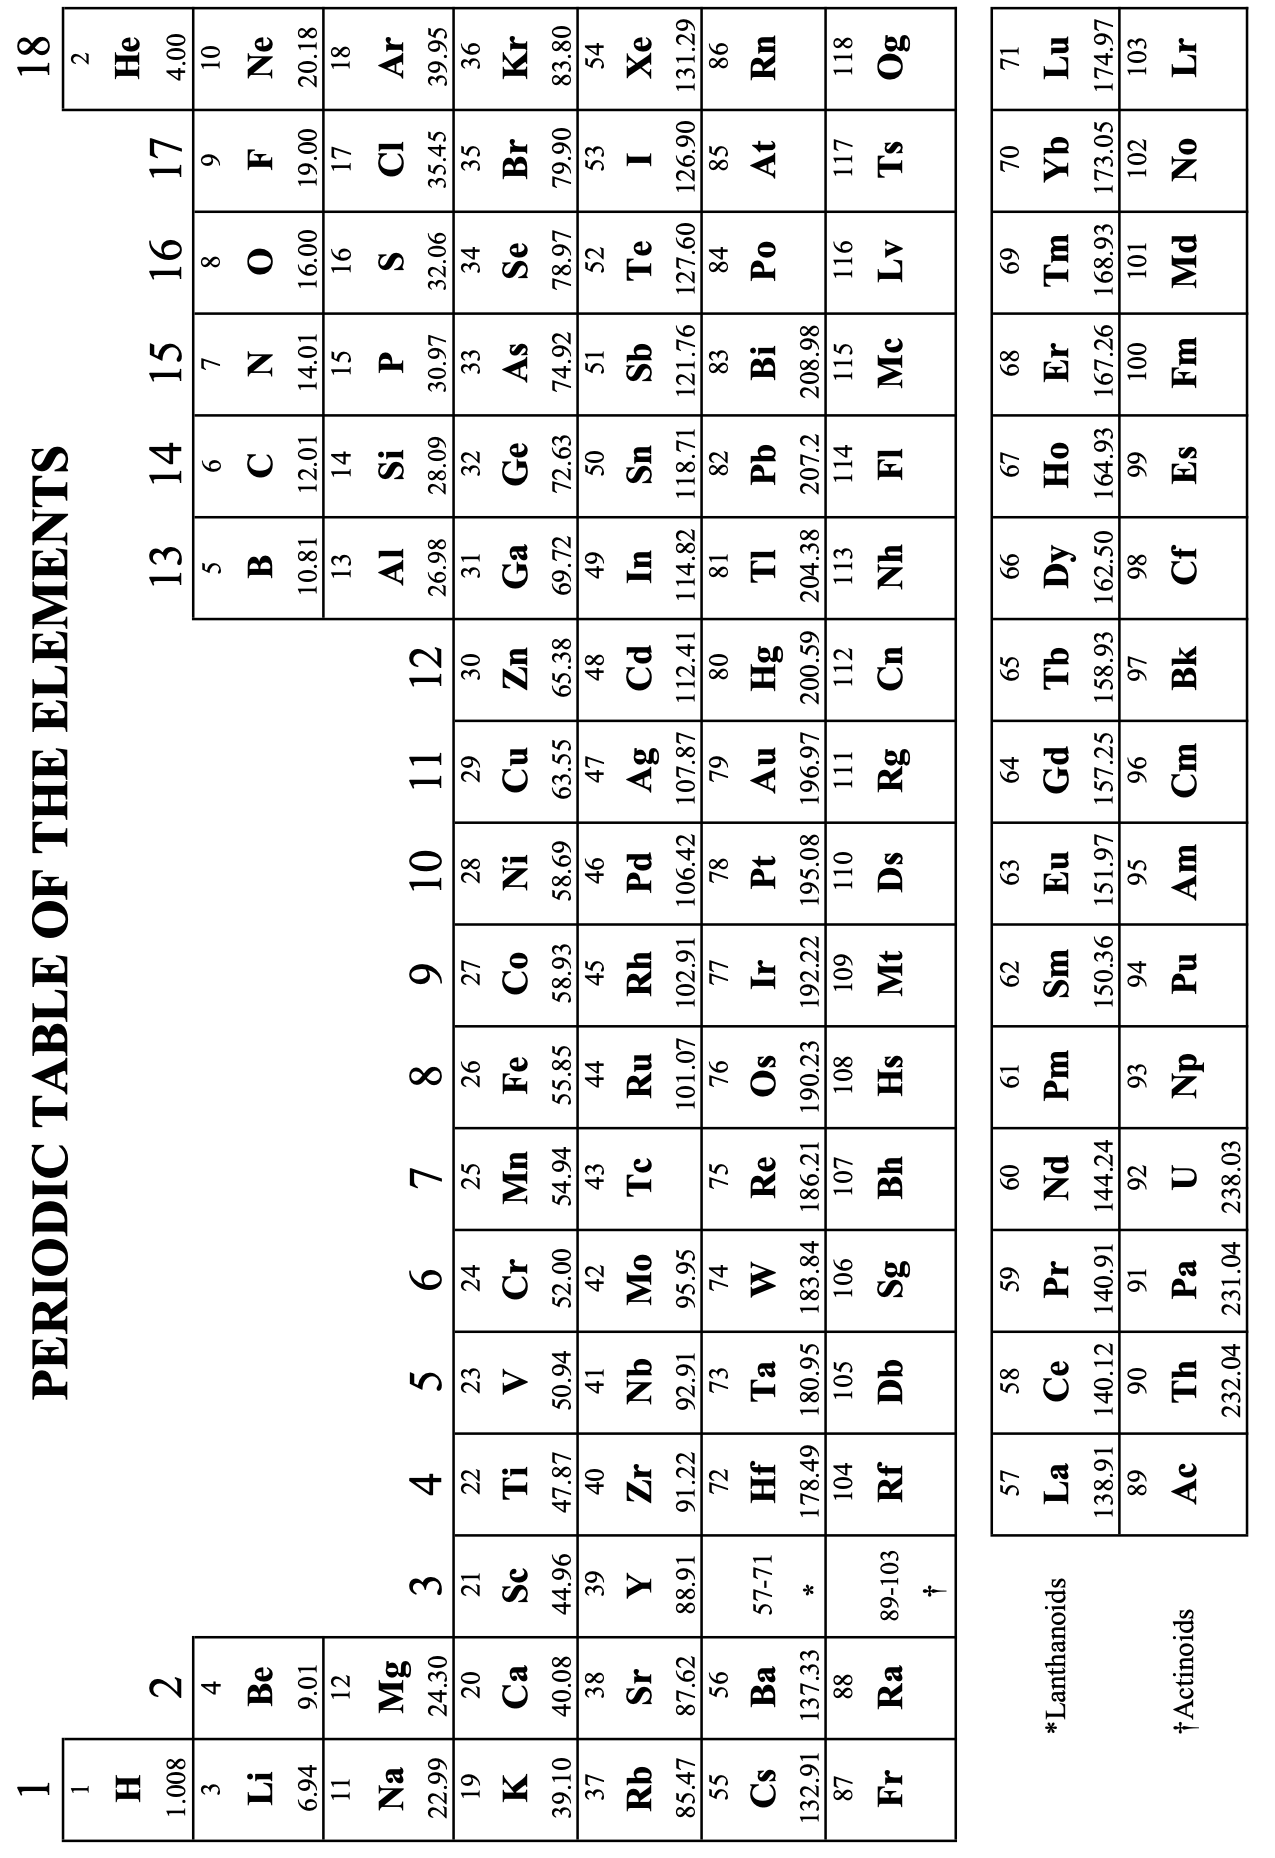
\includegraphics[width=0.65\textwidth]{periodic_table.png}
    \caption{Periodic Table of the Elements}
    \label{table:PeriodicTable}
\end{table}
\begin{table}[ht]
        \centering
        \begin{tabular}{l r}
        \begin{tabular}{c c c}
            Atomic Number & Symbol & Oxidation Numbers \\
            \hline
            1 & H & +1, -1 \\
            2 & He & None \\
            3 & Li & +1 \\
            4 & Be & +2 \\
            5 & B & +3 \\
            6 & C & +4, -2, -4 \\
            7 & N & +5, 4, 3, 2, +1, -3 \\
            8 & O & -2, -1 \\
            9 & F & -1 \\
            10 & Ne & None \\
            11 & Na & +1 \\
            12 & Mg & +2 \\
            13 & Al & +3 \\
            14 & Si & +4, -4 \\
            15 & P & +5, +3, -3 \\
            16 & S & +6, +4, +2, -2 \\
            17 & Cl & +7, +5, +3, +1, -1 \\
            18 & Ar & None \\
            19 & K & +1 \\
            20 & Ca & +2 \\
            21 & Sc & +3 \\
            22 & Ti & +4, +3, +2 \\
            23 & V & +5, +4, +3, +2 \\
            24 & Cr & +6, +3, +2 \\
            25 & Mn & +7, +6, +4, +3, +2 \\
            26 & Fe & +3, +2 \\
            27 & Co & +3, +2 \\
            28 & Ni & +2 \\
            29 & Cu & +2, +1 \\
            30 & Zn & +2 \\
            31 & Ga & +3 \\
            32 & Ge & +4, -4 \\
            33 & As & +5, +3, -3 \\
            34 & Se & +6, +4, -2 \\
            35 & Br & +5, +1, -1 \\
            36 & Kr & +4, +2 \\
            
        \end{tabular} & 
        \begin{tabular}{c c c}
            Atomic Number & Symbol & Oxidation Numbers \\
            \hline
            37 & Rb & +1 \\
            38 & Sr & +2 \\
            39 & Y & +3 \\
            40 & Zr & +4 \\
            41 & Nb & +5, +4 \\
            42 & Mo & +6, +4, +3 \\
            43 & Tc & +7, +6, +4 \\
            44 & Ru & +8, +6, +4, +3 \\
            45 & Rh & +4, +3, +2 \\
            46 & Pd & +4, +2 \\
            47 & Ag & +1 \\
            48 & Cd & +2 \\
            49 & In & +3 \\
            50 & Sn & +4, +2 \\
            51 & Sb & +5, +3, -3 \\
            52 & Te & +6, +4, -2 \\
            53 & I & +7, +5, +1, -1 \\
            54 & Xe & +6, +4, +2 \\
            55 & Cs & +1 \\
            56 & Ba & +2 \\
            57 & La & +3 \\
            72 & Hf & +4 \\
            73 & Ta & +5 \\
            74 & W & +6, +4 \\
            75 & Re & +7, +6, +4 \\
            76 & Os & +8, +6 \\
            77 & Ir & +4, +3 \\
            78 & Pt & +4, +2 \\
            79 & Au & +3, +1 \\
            80 & Hg & +2, +1 \\
            81 & Tl & +3, +1 \\
            82 & Pb & +4, +2 \\
            83 & Bi & +5, +3 \\
            84 & Po & +2 \\
            85 & At & -1 \\
            86 & Rn & None \\
        \end{tabular}\\
    \end{tabular}
        \caption{Oxidation Numbers for periods 1 through 5}
        \label{table:OxidationNumbers}
\end{table}
\begin{table}[pt]
        \centering
        \resizebox{0.9\textwidth}{!}{
        \begin{tabular}[t]{l r}
            \begin{tabular}{p{0.4\textwidth} l }
            Half Reaction & $E^\circ$ (V) \\
            \hline
            $\ce{Ag+(aq) + e- -> Ag(s)}$ & +0.80\\
            $\ce{AgBr(s) + e- -> Ag(s) + Br-(aq)}$ & +0.10\\
            $\ce{AgCl(s) + e- -> Ag(s) + Cl-(aq)}$ & +0.22\\
            $\ce{Ag(CN)2-(aq) + e- -> Ag(s) + 2 CN-(aq)}$ & -0.31\\
            $\ce{Ag2CrO4(s) + 2 e- -> 2 Ag(s) + CrO4^2-(aq)}$ & +0.45\\
            $\ce{AgI(s) + e- -> Ag(s) + I-(aq)}$ & -0.15\\
            $\ce{Ag2S2O3(s) + e- -> 2 Ag(s) + S2O3^2-(aq)}$ & +0.01\\
            $\ce{Al^3+(aq) + 3 e- -> Al(s)}$ & -1.66\\
            $\begin{multlined}[t][\linewidth]
                \ce{H3AsO4(aq) + 2 H+(aq) + 2 e- ->}\\ \ce{H3AsO3(aq) + H2(l)}
            \end{multlined}$ & +0.56\\
            $\ce{Ba^2+(aq) + 2 e- -> Ba(s)}$ & -2.90\\
            $\ce{BiO+(aq) + 2 H+(aq) + 3 e- -> Bi(s) + H2(l)}$ & +0.32\\
            $\ce{Br2(l) + 2 e- -> 2 Br-(aq)}$ & +1.07\\
            $\begin{multlined}[t][\linewidth]
                \ce{2 BrO3-(aq) + 12 H+(aq) + 10 e- ->}\\ \ce{Br2(l) + 6 H2(l)}
            \end{multlined}$ & +1.52\\
            $\ce{2 CO2(g) + 2 H+(aq) + 2 e- -> H2C2O4(aq)}$ & -0.49\\
            $\ce{Ca^2+(aq) + 2 e- -> Ca(s)}$ & -2.87\\
            $\ce{Cd^2+(aq) + 2 e- -> Cd(s)}$ & -0.40\\
            $\ce{Ce^4+(aq) + e- -> Ce^3+(aq)}$ & +1.61\\
            $\ce{Cl2(g) + 2 e- -> 2 Cl-(aq)}$ & +1.36\\
            $\begin{multlined}[t][\linewidth]
                \ce{2 HCl(aq) + 2 H+(aq) + 2 e- ->}\\ \ce{Cl2(g) + 2 H2(l)}
            \end{multlined}$ & +1.63\\
            $\begin{multlined}[t][\linewidth]
                \ce{ClO-(aq) + H2(l) + 2 e- ->}\\ \ce{Cl-(aq) + 2 OH-(aq)}
            \end{multlined}$& +0.89\\
            $\begin{multlined}[t][\linewidth]
                \ce{2 ClO3-(aq) + 12 H+(aq) + 10 e- ->}\\ \ce{Cl2(g) + 6 H2(l)}
            \end{multlined}$ & +1.47\\
            $\ce{Co^2+(aq) + 2 e- -> Co(s)}$ & -0.28\\
            $\ce{Co^3+(aq) + e- -> Co^2+(aq)}$ & +1.84\\
            $\ce{Cr^3+(aq) + 3 e- -> Cr(s)}$ & -0.74\\
            $\ce{Cr^3+(aq) + e- -> Cr^2+(aq)}$ & -0.41\\
            $\begin{multlined}[t][\linewidth]
                \ce{Cr2O7^2-(aq) + 14 H+(aq) + 6 e- ->}\\ \ce{2 Cr^3+(aq) + 7 H2(l)}
            \end{multlined}$ & +1.33\\
            $\begin{multlined}[t][\linewidth]
                \ce{CrO4^2-(aq) + 4 H2(l) + 3 e- ->}\\ \ce{Cr(OH)3(s) + 5 OH-(aq)}
            \end{multlined}$ & -0.13\\
            $\ce{Cu^2+(aq) + 2 e- -> Cu(s)}$ & +0.34\\
            $\ce{Cu^2+(aq) + e- -> Cu^+(aq)}$ & +0.15\\
            $\ce{Cu^+(aq) + e- -> Cu(s)}$ & +0.52\\
            $\ce{CuI(s) + e- -> Cu(s) + I^-(aq)}$ & -0.19\\
            $\ce{F2(g) + 2 e- -> 2 F^-(aq)}$ & +2.87 \\
            $\ce{Fe^2+(aq) + 2 e- -> Fe(s)}$ & -0.44 \\
            $\ce{Fe^3+(aq) + e- -> Fe^2+(aq)}$ & +0.77 \\
            $\ce{Fe(CN)6^3-(aq) + e- -> Fe(CN)6^4-(aq)}$ & +0.36\\
            $\ce{2 H+(aq) + 2 e- -> H2(g)}$ & 0.00\\
            $\ce{2 H2O(l) + 2 e- -> H2(g) + 2 OH-(aq)}$ & -0.83\\
            

        \end{tabular} &
        \begin{tabular}{p{0.4\textwidth} l }
            Half Reaction & $E^\circ$ (V) \\
            \hline
            $\ce{HO2-(aq) + H2O(l) + 2 e- -> 3 OH-(aq)}$ & +0.88\\
            $\ce{H2O2(aq) + 2 H+(aq) + 2 e- -> 2 H2(l)}$ & +1.78\\
            $\ce{Hg2^2+(aq) + 2 e- -> 2 Hg(l)}$ & +0.79\\
            $\ce{2 Hg2^2+(aq) + 2 e- -> Hg2^2+(aq)}$ & +0.92\\
            $\ce{Hg2^2+(aq) + 2 e- -> Hg(l)}$ & +0.85\\
            $\ce{I2(s) + 2 e- -> 2 I^-(aq)}$ & +0.54\\
            $\begin{multlined}[t][\linewidth]
                \ce{2 IO3^-(aq) + 12 H+(aq) + 10 e- ->}\\ \ce{I2(s) + 6 H2(l)}
            \end{multlined}$ & +1.20\\
            $\ce{K+(aq) + e- -> K(s)}$ & -2.92\\
            $\ce{Li+(aq) + e- -> Li(s)}$ & -3.05\\
            $\ce{Mg^2+(aq) + 2 e- -> Mg(s)}$ & -2.37\\
            $\ce{Mn^2+(aq) + 2 e- -> Mn(s)}$ & -1.18\\
            $\begin{multlined}[t][\linewidth]
                \ce{MnO2(s) + 4 H+(aq) + 2 e- ->}\\ \ce{Mn^2+(aq) + 2 H2(l)}
            \end{multlined}$ & +1.23\\
            $\begin{multlined}[t][\linewidth]
                \ce{MnO4^-(aq) + 8 H+(aq) + 5 e- ->}\\ \ce{Mn^2+(aq) + 4 H2(l)}
            \end{multlined}$ & +1.51\\
            $\begin{multlined}[t][\linewidth]
                \ce{MnO4^-(aq) + 2 H2(l) + 3 e- ->}\\ \ce{MnO2(s) + 4 OH-(aq)}
            \end{multlined}$ & +0.59\\
            $\ce{HNO2(aq) + H+(aq) + e- -> NO(g) + H2(l)}$ & +1.00\\
            $\begin{multlined}[t][\linewidth]
                \ce{N2(g) + 4 H2(l) + 4 e- ->}\\ \ce{4 OH-(aq) + N2H4(aq)}
            \end{multlined}$ & -1.16\\
            $\ce{N2(g) + 5 H+(aq) + 4 e- -> N2H5^+(aq)}$ & -0.23\\
            $\begin{multlined}[t][\linewidth]
                \ce{NO3^-(aq) + 4 H+(aq) + 3 e- ->}\\ \ce{NO(g) + 2 H2(l)}
            \end{multlined}$ & +0.96\\
            $\ce{Na+(aq) + e- -> Na(s)}$ & -2.71\\
            $\ce{Ni^2+(aq) + 2 e- -> Ni(s)}$ & -0.28\\
            $\ce{O2(g) + 4 H+(aq) + 4 e- -> 2 H2(l)}$ & +1.23\\
            $\ce{O2(g) + 2 H2(l) + 4 e- -> 4 OH-(aq)}$ & +0.40\\
            $\ce{O2(g) + 2 H+(aq) + 2 e- -> H2O2(aq)}$ & +0.68\\
            $\ce{O3(g) + 2 H+(aq) + 2 e- -> O2(g) + H2(l)}$ & +2.07\\
            $\ce{Pb^2+(aq) + 2 e- -> Pb(s)}$ & -0.13\\
            $\begin{multlined}[t][\linewidth]
                \ce{PbO2(s) + HSO4^-(aq) + 3 H+(aq) + 2 e- ->}\\ \ce{PbSO4(s) + 2 H2(l)}
            \end{multlined}$ & +1.69\\
            $\begin{multlined}[t][\linewidth]
                \ce{PbSO4(s) + H+(aq) + 2 e- ->}\\ \ce{Pb(s) + HSO4^-(aq)}
            \end{multlined}$ & -0.36\\
            $\ce{PtCl4^2-(aq) + 2 e- -> Pt(s) + 4 Cl^-(aq)}$ & +0.73\\
            $\ce{S(s) + 2 H+(aq) + 2 e- -> H2S(g)}$ & +0.14\\
            $\ce{H2SO3(aq) + 4 H+(aq) + 4 e- -> S(s) + 3 H2(l)}$ & +0.45\\
            $\begin{multlined}[t][\linewidth]
                \ce{HSO4^-(aq) + 3 H+(aq) + 2 e- ->}\\ \ce{H2SO3(aq) + H2(l)}
            \end{multlined}$ & +0.17\\
            $\ce{Sn^2+(aq) + 2 e- -> Sn(s)}$ & -0.14\\
            $\ce{Sn^4+(aq) + 2 e- -> Sn^2+(aq)}$ & +0.15\\
            $\begin{multlined}[t][\linewidth]
                \ce{VO2^+(aq) + 2 H+(aq) + e- ->}\\ \ce{VO^2+(aq) + H2(l)}
            \end{multlined}$ & +1.00\\
            $\ce{Zn^2+(aq) + 2 e- -> Zn(s)}$ & -0.76\\

        \end{tabular}\\
        \end{tabular}
        }
        \caption{Common Redox Half Reactions and their Standard Potentials}
        \label{table:StandardPotential}
\end{table}

\tablehead{%
\hline
Substance & $\Delta H_f^\circ$ (kJ/mol) & $\Delta G_f^\circ$ (kJ/mol) & $S^\circ$ (J/mol$\cdot$K) \\
\hline}
\tabletail{\hline}
\bottomcaption{Thermodynamic quantities for selected substances at 298.15 K}
\twocolumn
\tiny
\begin{supertabular}{llll}
    \ce{Al(s)} & 0 & 0 & 28.32 \\
    \ce{AlCl3(s)} & -705.6 & -630.0 & 109.3 \\
    \ce{Al2O3(s)} & -1669.8 & -1576.5 & 51.00 \\
    \ce{Ba(s)} & 0 & 0 & 63.2 \\
    \ce{BaCO3(s)} & -1216.3 & -1137.6 & 112.1 \\
    \ce{BaO(s)} & -553.5 & -525.1 & 70.42 \\
    \ce{Be(s)} & 0 & 0 & 9.44 \\
    \ce{BeO(s)} & -608.4 & -579.1 & 13.77 \\
    \ce{Be(OH)2(s)} & -905.8 & -817.9 & 50.21 \\
    \ce{Br(g)} & 111.8 & 82.38 & 174.9 \\
    \ce{Br-(aq)} & -120.9 & -102.8 & 80.71 \\
    \ce{Br2(g)} & 30.71 & 3.14 & 245.3 \\
    \ce{Br2(l)} & 0 & 0 & 152.3 \\
    \ce{HBr(g)} & -36.23 & -53.22 & 198.49 \\
    \ce{Ca(g)} & 179.3 & 145.5 & 154.8 \\
    \ce{Ca(s)} & 0 & 0 & 41.4 \\
    \ce{CaCO3(s, calcite)} & -1207.1 & -1128.76 & 92.88 \\
    \ce{CaCl2(s)} & -795.8 & -748.1 & 104.6 \\
    \ce{CaF2(s)} & -1219.6 & -1167.3 & 68.87 \\
    \ce{CaO(s)} & -635.5 & -604.17 & 39.75 \\
    \ce{Ca(OH)2(s)} & -986.2 & -898.5 & 83.4 \\
    \ce{CaSO4(s)} & -1434.0 & -1321.8 & 106.7 \\
    \ce{C(g)} & 718.4 & 672.9 & 158.0 \\
    \ce{C(s, diamond)} & 1.88 & 2.84 & 2.43 \\
    \ce{C(s, graphite)} & 0 & 0 & 5.69 \\
    \ce{CCl4(g)} & -106.7 & -64.0 & 309.4 \\
    \ce{CCl4(l)} & -139.3 & -68.6 & 214.4 \\
    \ce{CF4(g)} & -679.9 & -635.1 & 262.3 \\
    \ce{CH4(g)} & -74.8 & -50.8 & 186.3 \\
    \ce{C2H2(g)} & 226.77 & 209.2 & 200.8 \\
    \ce{C2H4(g)} & 52.30 & 68.11 & 219.4 \\
    \ce{C2H6(g)} & -84.68 & -32.89 & 229.5 \\
    \ce{C3H8(g)} & -103.85 & -23.47 & 269.9 \\
    \ce{C4H10(g)} & -124.73 & -15.71 & 310.0 \\
    \ce{C4H10(l)} & -147.6 & -15.0 & 231.0 \\
    \ce{C6H6(g)} & 82.9 & 129.7 & 269.2 \\
    \ce{C6H6(l)} & 49.0 & 124.5 & 172.8 \\
    \ce{CH3OH(g)} & -201.2 & -161.9 & 237.6 \\
    \ce{CH3OH(l)} & -238.6 & -166.23 & 126.8 \\
    \ce{C2H5OH(g)} & -235.1 & -168.5 & 282.7 \\
    \ce{C2H5OH(l)} & -277.7 & -174.76 & 160.7 \\
    \ce{C6H12O6(s)} & -1273.02 & -910.4 & 212.1 \\
    \ce{CO(g)} & -110.5 & -137.2 & 197.9 \\
    \ce{CO2(g)} & -393.5 & -394.4 & 213.6 \\
    \ce{CH3COOH(l)} & -487.0 & -392.4 & 159.8 \\
    \ce{Cs(g)} & 76.50 & 49.53 & 175.6 \\
    \ce{Cs(l)} & 2.09 & 0.03 & 92.07 \\
    \ce{Cs(s)} & 0 & 0 & 85.15 \\
    \ce{CsCl(s)} & -442.8 & -414.4 & 101.2 \\
    \ce{Cl(g)} & 121.7 & 105.7 & 165.2 \\
    \ce{Cl-(aq)} & -167.2 & -131.2 & 56.5 \\
    \ce{Cl2(g)} & 0 & 0 & 222.96 \\
    \ce{HCl(aq)} & -167.2 & -131.2 & 56.5 \\
    \ce{HCl(g)} & -92.30 & -95.27 & 186.69 \\
    \ce{Cr(g)} & 397.5 & 352.6 & 174.2 \\
    \ce{Cr(s)} & 0 & 0 & 23.6 \\
    \ce{Cr2O3(s)} & -1139.7 & -1058.1 & 81.2 \\
    \ce{Co(g)} & 439 & 393 & 179 \\
    \ce{Co(s)} & 0 & 0 & 28.4 \\
    \ce{Cu(g)} & 338.4 & 298.6 & 166.3 \\
    \ce{Cu(s)} & 0 & 0 & 33.30 \\
    \ce{CuCl2(s)} & -205.9 & -161.7 & 108.1 \\
    \ce{CuO(s)} & -156.1 & -128.3 & 42.59 \\
    \ce{Cu2O(s)} & -170.7 & -147.9 & 92.36 \\
    \ce{F(g)} & 80.0 & 61.9 & 158.7 \\
    \ce{F-(aq)} & -332.6 & -278.8 & -13.8 \\
    \ce{F2(g)} & 0 & 0 & 202.7 \\
    \ce{HF(g)} & -268.61 & -270.70 & 173.51 \\
    \ce{H(g)} & 217.94 & 203.26 & 114.60 \\
    \ce{H+(aq)} & 0 & 0 & 0 \\
    \ce{H+(g)} & 1536.2 & 1517.0 & 108.9 \\
    \ce{H2(g)} & 0 & 0 & 130.58 \\
    \ce{I(g)} & 106.60 & 70.16 & 180.66 \\
    \ce{I-(g)} & -55.19 & -51.57 & 111.3 \\
    \ce{I2(g)} & 62.25 & 19.37 & 260.57 \\
    \ce{I2(s)} & 0 & 0 & 116.73 \\
    \ce{HI(g)} & 25.94 & 1.30 & 206.3 \\
    \ce{Fe(g)} & 415.5 & 369.8 & 180.5 \\
    \ce{Fe(s)} & 0 & 0 & 27.15 \\
    \ce{Fe^2+(aq)} & -87.86 & -84.93 & 113.4 \\
    \ce{Fe^3+(aq)} & -47.69 & -10.54 & 293.3 \\
    \ce{FeCl2(s)} & -341.8 & -302.3 & 117.9 \\
    \ce{FeCl3(s)} & -400 & -334 & 142.3 \\
    \ce{FeO(s)} & -271.9 & -255.2 & 60.75 \\
    \ce{Fe2O3(s)} & -822.16 & -740.98 & 89.96 \\
    \ce{Fe3O4(s)} & -1117.1 & -1014.2 & 146.4 \\
    \ce{FeS2(s)} & -171.5 & -160.1 & 52.92 \\
    \ce{Pb(s)} & 0 & 0 & 68.85 \\
    \ce{PbBr2(s)} & -277.4 & -260.7 & 161 \\
    \ce{PbCO3(s)} & -699.1 & -625.5 & 131.0 \\
    \ce{Pb(NO3)2(aq)} & -421.3 & -246.9 & 303.3 \\
    \ce{Pb(NO3)2(s)} & -451.9 & --- & --- \\
    \ce{PbO(s)} & -217.3 & -187.9 & 68.70 \\
    \ce{Li(g)} & 159.3 & 126.6 & 138.8 \\
    \ce{Li(s)} & 0 & 0 & 29.09 \\
    \ce{Li+(aq)} & -278.5 & -273.4 & 12.2 \\
    \ce{Li+(g)} & 685.7 & 648.5 & 133.0 \\
    \ce{LiCl(s)} & -408.3 & -384.0 & 59.30 \\
    \ce{Mg(g)} & 147.1 & 112.5 & 148.6 \\
    \ce{Mg(s)} & 0 & 0 & 32.51 \\
    \ce{MgCl2(s)} & -641.6 & -592.1 & 89.6 \\
    \ce{MgO(s)} & -601.8 & -569.6 & 26.8 \\
    \ce{Mg(OH)2(s)} & -924.7 & -833.7 & 63.24 \\
    \ce{Mn(g)} & 280.7 & 238.5 & 173.6 \\
    \ce{Mn(s)} & 0 & 0 & 32.0 \\
    \ce{MnO(s)} & -385.2 & -362.9 & 59.7 \\
    \ce{MnO2(s)} & -519.6 & -464.8 & 53.14 \\
    \ce{MnO4-(aq)} & -541.4 & -447.2 & 191.2 \\
    \ce{Hg(g)} & 60.83 & 31.76 & 174.89 \\
    \ce{Hg(l)} & 0 & 0 & 77.40 \\
    \ce{HgCl2(s)} & -230.1 & -184.0 & 144.5 \\
    \ce{Hg2Cl2(s)} & -264.9 & -210.5 & 192.5 \\
    \ce{Ni(g)} & 429.7 & 384.5 & 182.1 \\
    \ce{Ni(s)} & 0 & 0 & 29.9 \\
    \ce{NiCl2(s)} & -305.3 & -259.0 & 97.65 \\
    \ce{NiO(s)} & -239.7 & -211.7 & 37.99 \\
    \ce{N(g)} & 472.7 & 455.5 & 153.3 \\
    \ce{N2(g)} & 0 & 0 & 191.50 \\
    \ce{NH3(aq)} & -80.29 & -26.50 & 111.3 \\
    \ce{NH3(g)} & -46.19 & -16.66 & 192.5 \\
    \ce{NH4+(aq)} & -132.5 & -79.31 & 113.4 \\
    \ce{N2H4(g)} & 95.40 & 159.4 & 238.5 \\
    \ce{NH4CN(s)} & 0.4 & --- & --- \\
    \ce{NH4Cl(s)} & -314.4 & -203.0 & 94.6 \\
    \ce{NH4NO3(s)} & -365.6 & -184.0 & 151 \\
    \ce{NO(g)} & 90.37 & 86.71 & 210.62 \\
    \ce{NO2(g)} & 33.84 & 51.84 & 240.45 \\
    \ce{N2O(g)} & 81.6 & 103.59 & 220.0 \\
    \ce{N2O4(g)} & 9.66 & 98.28 & 304.3 \\
    \ce{NOCl(g)} & 52.6 & 66.3 & 264 \\
    \ce{HNO3(aq)} & -206.6 & -110.5 & 146 \\
    \ce{HNO3(g)} & -134.3 & -73.94 & 266.4 \\
    \ce{O(g)} & 247.5 & 230.1 & 161.0 \\
    \ce{O2(g)} & 0 & 0 & 205.0 \\
    \ce{O3(g)} & 142.3 & 163.4 & 237.6 \\
    \ce{OH-(aq)} & -230.0 & -157.3 & -10.7 \\
    \ce{H2O(g)} & -241.82 & -228.57 & 188.83 \\
    \ce{H2O(l)} & -285.83 & -237.13 & 69.91 \\
    \ce{H2O2(g)} & -136.10 & -105.48 & 232.9 \\
    \ce{H2O2(l)} & -187.8 & -120.4 & 109.6 \\
    \ce{P(g)} & 316.4 & 280.0 & 163.2 \\
    \ce{P2(g)} & 144.3 & 103.7 & 218.1 \\
    \ce{P4(g)} & 58.9 & 24.4 & 280 \\
    \ce{P4(s, red)} & -17.46 & -12.03 & 22.85 \\
    \ce{P4(s, white)} & 0 & 0 & 41.08 \\
    \ce{PCl3(g)} & -288.07 & -269.6 & 311.7 \\
    \ce{PCl3(l)} & -319.6 & -272.4 & 217 \\
    \ce{PF5(g)} & -1594.4 & -1520.7 & 300.8 \\
    \ce{PH3(g)} & 5.4 & 13.4 & 210.2 \\
    \ce{P4O6(s)} & -1640.1 & --- & --- \\
    \ce{P4O10(s)} & -2940.1 & -2675.2 & 228.9 \\
    \ce{POCl3(g)} & -542.2 & -502.5 & 325 \\
    \ce{POCl3(l)} & -597.0 & -520.9 & 222 \\
    \ce{H3PO4(aq)} & -1288.3 & -1142.6 & 158.2 \\
    \ce{K(g)} & 89.99 & 61.17 & 160.2 \\
    \ce{K(s)} & 0 & 0 & 64.67 \\
    \ce{K+(aq)} & -252.4 & -283.3 & 102.5 \\
    \ce{K+(g)} & 514.2 & 481.2 & 154.5 \\
    \ce{KCl(s)} & -435.9 & -408.3 & 82.7 \\
    \ce{KClO3(s)} & -391.2 & -289.9 & 143.0 \\
    \ce{KClO3(aq)} & -349.5 & -284.9 & 265.7 \\
    \ce{K2CO3(s)} & -1150.18 & -1064.58 & 155.44 \\
    \ce{KNO3(s)} & -492.70 & -393.13 & 132.9 \\
    \ce{K2O(s)} & -363.2 & -322.1 & 94.14 \\
    \ce{KO2(s)} & -284.5 & -240.6 & 122.5 \\
    \ce{K2O2(s)} & -495.8 & -429.8 & 113.0 \\
    \ce{KOH(s)} & -424.7 & -378.9 & 78.91 \\
    \ce{KOH(aq)} & -482.4 & -440.5 & 91.6 \\
    \ce{Rb(g)} & 85.8 & 55.8 & 170.0 \\
    \ce{Rb(s)} & 0 & 0 & 76.78 \\
    \ce{RbCl(s)} & -430.5 & -412.0 & 92 \\
    \ce{RbClO3(s)} & -392.4 & -292.0 & 152 \\
    \ce{Sc(g)} & 377.8 & 336.1 & 174.7 \\
    \ce{Sc(s)} & 0 & 0 & 34.6 \\
    \ce{H2Se(g)} & 29.7 & 15.9 & 219.0 \\
    \ce{Si(g)} & 368.2 & 323.9 & 167.8 \\
    \ce{Si(s)} & 0 & 0 & 18.7 \\
    \ce{SiC(s)} & -73.22 & -70.85 & 16.61 \\
    \ce{SiCl4(l)} & -640.1 & -572.8 & 239.3 \\
    \ce{SiO2(s, quartz)} & -910.9 & -856.5 & 41.84 \\
    \ce{Ag(s)} & 0 & 0 & 42.55 \\
    \ce{Ag+(aq)} & 105.90 & 77.11 & 73.93 \\
    \ce{AgCl(s)} & -127.0 & -109.70 & 96.11 \\
    \ce{Ag2O(s)} & -31.05 & -11.20 & 121.3 \\
    \ce{AgNO3(s)} & -124.4 & -33.41 & 140.9 \\
    \ce{Na(g)} & 107.7 & 77.3 & 153.7 \\
    \ce{Na(s)} & 0 & 0 & 51.45 \\
    \ce{Na+(aq)} & -240.1 & -261.9 & 59.0 \\
    \ce{Na+(g)} & 609.3 & 574.3 & 148.0 \\
    \ce{NaBr(aq)} & -360.6 & -364.7 & 141.00 \\
    \ce{NaBr(s)} & -361.4 & -349.3 & 86.82 \\
    \ce{Na2CO3(s)} & -1130.9 & -1047.7 & 136.0 \\
    \ce{NaCl(aq)} & -407.1 & -393.0 & 115.5 \\
    \ce{NaCl(g)} & -181.4 & -201.3 & 229.8 \\
    \ce{NaCl(s)} & -410.9 & -384.0 & 72.33 \\
    \ce{NaHCO3(s)} & -947.7 & -851.8 & 102.1 \\
    \ce{NaNO3(aq)} & -446.2 & -372.4 & 207 \\
    \ce{NaNO3(s)} & -467.9 & -367.0 & 116.5 \\
    \ce{NaOH(aq)} & -469.6 & -419.2 & 49.8 \\
    \ce{NaOH(s)} & -425.6 & -379.5 & 64.46 \\
    \ce{Na2SO4(s)} & -1387.1 & -1270.2 & 149.6 \\
    \ce{SrO(s)} & -592.0 & -561.9 & 54.9 \\
    \ce{Sr(g)} & 164.4 & 110.0 & 164.6 \\
    \ce{S(s, rhombic)} & 0 & 0 & 31.88 \\
    \ce{S8(g)} & 102.3 & 49.7 & 430.9 \\
    \ce{SO2(g)} & -296.9 & -300.4 & 248.5 \\
    \ce{SO3(g)} & -395.2 & -370.4 & 256.2 \\
    \ce{SO4^2-(aq)} & -909.3 & -744.5 & 20.1 \\
    \ce{SOCl2(l)} & -245.6 & --- & --- \\
    \ce{H2S(g)} & -20.17 & -33.01 & 205.6 \\
    \ce{H2SO4(aq)} & -909.3 & -744.5 & 20.1 \\
    \ce{H2SO4(l)} & -814.0 & -689.9 & 156.1 \\
    \ce{Ti(g)} & 468 & 422 & 180.3 \\
    \ce{Ti(s)} & 0 & 0 & 30.76 \\
    \ce{TiCl4(g)} & -763.2 & -726.8 & 354.9 \\
    \ce{TiCl4(l)} & -804.2 & -728.1 & 221.9 \\
    \ce{TiO2(s)} & -944.7 & -889.4 & 50.29 \\
    \ce{V(g)} & 514.2 & 453.1 & 182.2 \\
    \ce{V(s)} & 0 & 0 & 28.9 \\
    \ce{Zn(g)} & 130.7 & 95.2 & 160.9 \\
    \ce{Zn(s)} & 0 & 0 & 41.63 \\
    \ce{ZnCl2(s)} & -415.1 & -369.4 & 111.5 \\
    \ce{ZnO(s)} & -348.0 & -318.2 & 43.9 \\
    \hline
\end{supertabular}
\onecolumn
\normalsize
\clearpage
\begin{table}[ht]
    \centering
    \begin{tabular}{l r }
        \begin{tabular}{l l l }
            Bond & Energy (kJ/mol) & Length (pm) \\
            \hline
            $\chemfig{H-H}$ & 432 & 75 \\
            $\chemfig{H-F}$ & 565 & 92 \\
            $\chemfig{H-Cl}$ & 427 & 127 \\
            $\chemfig{H-Br}$ & 363 & 141 \\
            $\chemfig{H-I}$ & 295 & 161 \\
            $\chemfig{C-H}$ & 413 & 109 \\
            $\chemfig{C-F}$ & 485 & 135 \\
            $\chemfig{C-Cl}$ & 339 & 177 \\
            $\chemfig{C-Br}$ & 276 & 194 \\
            $\chemfig{C-I}$ & 240 & 214 \\
            $\chemfig{C-C}$ & 347 & 154 \\
            $\chemfig{C=C}$ & 614 & 134 \\
            $\chemfig{C~C}$ & 839 & 120 \\
            $\chemfig{C-N}$ & 305 & 143 \\
            $\chemfig{C=N}$ & 615 & 138 \\
            $\chemfig{C~N}$ & 891 & 116 \\
            $\chemfig{N-H}$ & 391 & 101 \\
            $\chemfig{N-F}$ & 272 & 136 \\
            $\chemfig{N-Cl}$ & 200 & 175 \\
            $\chemfig{N-Br}$ & 243 & 189 \\
            $\chemfig{N-N}$ & 160 & 145 \\
            $\chemfig{N=N}$ & 418 & 125 \\
            $\chemfig{N~N}$ & 941 & 110 \\
            $\chemfig{O-H}$ & 467 & 96 \\
        \end{tabular} &
        \begin{tabular}{l l l }
            Bond & Energy (kJ/mol) & Length (pm) \\
            \hline
            $\chemfig{O-F}$ & 190 & 142 \\
            $\chemfig{O-Cl}$ & 203 & 172 \\
            $\chemfig{O-I}$ & 234 & 206 \\
            $\chemfig{O-O}$ & 146 & 148 \\
            $\chemfig{O=O}$ & 495 & 121 \\
            $\chemfig{C-O}$ & 358 & 143 \\
            $\chemfig{C=O}$ & 745\footnotemark & 120 \\
            $\chemfig{C~O}$ & 1072 & 113 \\
            $\chemfig{F-F}$ & 154 & 142 \\
            $\chemfig{F-Cl}$ & 253 & 142 \\
            $\chemfig{F-Br}$ & 237 & 191 \\
            $\chemfig{F-I}$ & 273 & 191 \\
            $\chemfig{Cl-Cl}$ & 239 & 199 \\
            $\chemfig{Cl-Br}$ & 218 & 214 \\
            $\chemfig{Cl-I}$ & 208 & 232 \\
            $\chemfig{Br-Br}$ & 193 & 228 \\
            $\chemfig{Br-I}$ & 175 & 247 \\
            $\chemfig{I-I}$ & 149 & 267 \\
            $\chemfig{S-H}$ & 363 & 134 \\
            $\chemfig{S-F}$ & 327 & 156 \\
            $\chemfig{S-Cl}$ & 253 & 207 \\
            $\chemfig{S-Br}$ & 218 & 216 \\
            $\chemfig{S-O}$ & 523 & 143 \\
            $\chemfig{S-S}$ & 266 & 205 \\
        \end{tabular}
    \end{tabular}
    \caption{Bond Energies and Lengths for Selected Bonds}
\end{table}
\footnotetext{$\chemfig{C=O}$ bond energy in $\ce{CO2}$ is 799 kJ/mol}
\clearpage
\begin{table}[ht]
    \centering
    \resizebox{\textwidth}{!}{
    \begin{tabular}{| l | c | c c c | c c c | c c c c c | c c | }
        \hline
    & & \multicolumn{3}{c|}{Alkali}  & \multicolumn{3}{c|}{Alkaline Earth} & \multicolumn{5}{c|}{Transition} & \multicolumn{2}{c|}{Post-Transition} \\
    \hline
    & \ce{NH4+} & \ce{Li+} & \ce{Na+} & \ce{K+} & \ce{Mg^2+} & \ce{Ca^2+} & \ce{Ba^2+} & \ce{Fe^2+} & \ce{Fe^3+} & \ce{Cu^2+} & \ce{Ag+} & \ce{Zn^2+} & \ce{Pb^2+} & \ce{Al^3+} \\
    \hline
    \ce{F-} &\cmark &\cmark &\cmark &\cmark &\xmark &\xmark &$-$ &$-$ &$-$ &\cmark &\cmark &\cmark &\xmark &$-$ \\
    \ce{Cl-} &\cmark &\cmark &\cmark &\cmark &\cmark &\cmark &\cmark &\cmark &\cmark &\cmark &\xmark &\cmark &\xmark &\cmark \\
    \ce{Br-} &\cmark &\cmark &\cmark &\cmark &\cmark &\cmark &\cmark &\cmark &\cmark &\cmark &\xmark &\cmark &$-$ &\cmark \\
    \ce{I-} &\cmark &\cmark &\cmark &\cmark &\cmark &\cmark &\cmark &\cmark & & &\xmark &\cmark &\xmark &\cmark \\
    \ce{ClO3-} &\cmark &\cmark &\cmark &\cmark &\cmark &\cmark &\cmark & &\cmark & &\cmark & &\cmark &\cmark \\
    \ce{OH-} &\cmark &\cmark &\cmark &\cmark &\xmark &$-$ &\cmark &\xmark &\xmark &\xmark &$-$ &\xmark &\xmark &\xmark \\
    \ce{S^2-} &\cmark &\cmark &\cmark &\cmark & &$-$ &$-$ & &\xmark &\xmark &\xmark &\xmark &\xmark &\xmark \\
    \ce{SO2^2-} &\cmark &\cmark &\cmark &\cmark &\cmark &\xmark &\xmark & & & &\xmark &\xmark &\xmark & \\
    \ce{SO4^2-} &\cmark &\cmark &\cmark &\cmark &\cmark &$-$ &\xmark &\cmark &\cmark &\cmark &$-$ &\cmark &\xmark &\cmark \\
    \ce{CO3^2-} &\cmark &\cmark &\cmark &\cmark &\xmark &\xmark &\xmark &\xmark & &\xmark &\xmark &\xmark &\xmark & \\
    \ce{NO2-} &\cmark &\cmark &\cmark &\cmark &\cmark &\cmark &\cmark & & & &\xmark & &\cmark & \\
    \ce{NO3-} &\cmark &\cmark &\cmark &\cmark &\cmark &\cmark &\cmark &\cmark &\cmark &\cmark &\cmark &\cmark &\cmark &\cmark \\
    \ce{PO4^3-} &\cmark &\xmark &\cmark &\cmark &\xmark &\xmark &\xmark &\xmark &\xmark &\xmark &\xmark &\xmark &\xmark &\xmark \\
    \ce{CrO4^2-} &\cmark &\cmark &\cmark &\cmark &\cmark & &\cmark &\xmark &\xmark &\xmark &\xmark &\xmark &\xmark & \\
    \ce{CH3CO2-} &\cmark &\cmark &\cmark &\cmark &\cmark &\cmark &\cmark &\cmark &\cmark &\cmark &\cmark &\cmark &\cmark &$-$ \\
    \hline
    \end{tabular}
    }
    \caption{Solubility of Common Salts in Water at 25$^\circ$C. `{\cmark}' indicates that the salt is soluble ($>1$g/100 mL), `{\xmark}' indicates that it is insoluble ($<0.01$g/100 mL) and `$-$' indicates that the salt is slightly soluble (0.01-1 g/100 mL).}
\end{table}


\clearpage
\section*{About this Document}
This document is a compilation of all the notes made from the teachers slides presentations in addition to figures, equations, explanations, tables and more from me and other sources. The goal I have is for this document to be a comprehensive review of all the material covered in AP Chemistry, and to be a living document that can be updated and added on to. For this the source code is available on \textbf{GitHub} at https://github.com/EnderBuilds/APChemistryPacket, where you are free to contribute by adding more information, fixing errors, improving formatting and more. If you have any questions or suggestions, feel free to reach out. I hope that this document had something to offer, weather it be a new way to understand a concept, a useful figure, or just a comprehensive review of the material. I wish you good luck on your journey through AP Chemistry.\\
Sincerely,\\
The Author
\end{document}